% Options for packages loaded elsewhere
\PassOptionsToPackage{unicode}{hyperref}
\PassOptionsToPackage{hyphens}{url}
\documentclass[
]{article}
\usepackage{xcolor}
\usepackage{amsmath,amssymb}
\setcounter{secnumdepth}{-\maxdimen} % remove section numbering
\usepackage{iftex}
\ifPDFTeX
  \usepackage[T1]{fontenc}
  \usepackage[utf8]{inputenc}
  \usepackage{textcomp} % provide euro and other symbols
\else % if luatex or xetex
  \usepackage{unicode-math} % this also loads fontspec
  \defaultfontfeatures{Scale=MatchLowercase}
  \defaultfontfeatures[\rmfamily]{Ligatures=TeX,Scale=1}
\fi
\usepackage{lmodern}
\ifPDFTeX\else
  % xetex/luatex font selection
\fi
% Use upquote if available, for straight quotes in verbatim environments
\IfFileExists{upquote.sty}{\usepackage{upquote}}{}
\IfFileExists{microtype.sty}{% use microtype if available
  \usepackage[]{microtype}
  \UseMicrotypeSet[protrusion]{basicmath} % disable protrusion for tt fonts
}{}
\makeatletter
\@ifundefined{KOMAClassName}{% if non-KOMA class
  \IfFileExists{parskip.sty}{%
    \usepackage{parskip}
  }{% else
    \setlength{\parindent}{0pt}
    \setlength{\parskip}{6pt plus 2pt minus 1pt}}
}{% if KOMA class
  \KOMAoptions{parskip=half}}
\makeatother
\usepackage{color}
\usepackage{fancyvrb}
\newcommand{\VerbBar}{|}
\newcommand{\VERB}{\Verb[commandchars=\\\{\}]}
\DefineVerbatimEnvironment{Highlighting}{Verbatim}{commandchars=\\\{\}}
% Add ',fontsize=\small' for more characters per line
\newenvironment{Shaded}{}{}
\newcommand{\AlertTok}[1]{\textcolor[rgb]{1.00,0.00,0.00}{\textbf{#1}}}
\newcommand{\AnnotationTok}[1]{\textcolor[rgb]{0.38,0.63,0.69}{\textbf{\textit{#1}}}}
\newcommand{\AttributeTok}[1]{\textcolor[rgb]{0.49,0.56,0.16}{#1}}
\newcommand{\BaseNTok}[1]{\textcolor[rgb]{0.25,0.63,0.44}{#1}}
\newcommand{\BuiltInTok}[1]{\textcolor[rgb]{0.00,0.50,0.00}{#1}}
\newcommand{\CharTok}[1]{\textcolor[rgb]{0.25,0.44,0.63}{#1}}
\newcommand{\CommentTok}[1]{\textcolor[rgb]{0.38,0.63,0.69}{\textit{#1}}}
\newcommand{\CommentVarTok}[1]{\textcolor[rgb]{0.38,0.63,0.69}{\textbf{\textit{#1}}}}
\newcommand{\ConstantTok}[1]{\textcolor[rgb]{0.53,0.00,0.00}{#1}}
\newcommand{\ControlFlowTok}[1]{\textcolor[rgb]{0.00,0.44,0.13}{\textbf{#1}}}
\newcommand{\DataTypeTok}[1]{\textcolor[rgb]{0.56,0.13,0.00}{#1}}
\newcommand{\DecValTok}[1]{\textcolor[rgb]{0.25,0.63,0.44}{#1}}
\newcommand{\DocumentationTok}[1]{\textcolor[rgb]{0.73,0.13,0.13}{\textit{#1}}}
\newcommand{\ErrorTok}[1]{\textcolor[rgb]{1.00,0.00,0.00}{\textbf{#1}}}
\newcommand{\ExtensionTok}[1]{#1}
\newcommand{\FloatTok}[1]{\textcolor[rgb]{0.25,0.63,0.44}{#1}}
\newcommand{\FunctionTok}[1]{\textcolor[rgb]{0.02,0.16,0.49}{#1}}
\newcommand{\ImportTok}[1]{\textcolor[rgb]{0.00,0.50,0.00}{\textbf{#1}}}
\newcommand{\InformationTok}[1]{\textcolor[rgb]{0.38,0.63,0.69}{\textbf{\textit{#1}}}}
\newcommand{\KeywordTok}[1]{\textcolor[rgb]{0.00,0.44,0.13}{\textbf{#1}}}
\newcommand{\NormalTok}[1]{#1}
\newcommand{\OperatorTok}[1]{\textcolor[rgb]{0.40,0.40,0.40}{#1}}
\newcommand{\OtherTok}[1]{\textcolor[rgb]{0.00,0.44,0.13}{#1}}
\newcommand{\PreprocessorTok}[1]{\textcolor[rgb]{0.74,0.48,0.00}{#1}}
\newcommand{\RegionMarkerTok}[1]{#1}
\newcommand{\SpecialCharTok}[1]{\textcolor[rgb]{0.25,0.44,0.63}{#1}}
\newcommand{\SpecialStringTok}[1]{\textcolor[rgb]{0.73,0.40,0.53}{#1}}
\newcommand{\StringTok}[1]{\textcolor[rgb]{0.25,0.44,0.63}{#1}}
\newcommand{\VariableTok}[1]{\textcolor[rgb]{0.10,0.09,0.49}{#1}}
\newcommand{\VerbatimStringTok}[1]{\textcolor[rgb]{0.25,0.44,0.63}{#1}}
\newcommand{\WarningTok}[1]{\textcolor[rgb]{0.38,0.63,0.69}{\textbf{\textit{#1}}}}
\usepackage{longtable,booktabs,array}
\usepackage{caption}
\captionsetup[table]{skip=6pt}
\newcounter{none} % for unnumbered tables
\usepackage{calc} % for calculating minipage widths
% Correct order of tables after \paragraph or \subparagraph
\usepackage{etoolbox}
\makeatletter
\patchcmd\longtable{\par}{\if@noskipsec\mbox{}\fi\par}{}{}
\makeatother
% Allow footnotes in longtable head/foot
\IfFileExists{footnotehyper.sty}{\usepackage{footnotehyper}}{\usepackage{footnote}}
\makesavenoteenv{longtable}
\usepackage{graphicx}
\makeatletter
\newsavebox\pandoc@box
\newcommand*\pandocbounded[1]{% scales image to fit in text height/width
  \sbox\pandoc@box{#1}%
  \Gscale@div\@tempa{\textheight}{\dimexpr\ht\pandoc@box+\dp\pandoc@box\relax}%
  \Gscale@div\@tempb{\linewidth}{\wd\pandoc@box}%
  \ifdim\@tempb\p@<\@tempa\p@\let\@tempa\@tempb\fi% select the smaller of both
  \ifdim\@tempa\p@<\p@\scalebox{\@tempa}{\usebox\pandoc@box}%
  \else\usebox{\pandoc@box}%
  \fi%
}
% Set default figure placement to htbp
\def\fps@figure{htbp}
\makeatother
\setlength{\emergencystretch}{3em} % prevent overfull lines
\providecommand{\tightlist}{%
  \setlength{\itemsep}{0pt}\setlength{\parskip}{0pt}}
\usepackage{bookmark}
\IfFileExists{xurl.sty}{\usepackage{xurl}}{} % add URL line breaks if available
\urlstyle{same}
% fallback for those not using the hyperref driver hyperxmp:
\makeatletter
\@ifundefined{xmpquote}{\newcommand{\xmpquote}[1]{#1}}{}
\makeatother
\hypersetup{
  hidelinks,
  pdfcreator={LaTeX via pandoc}}

\author{}
\date{}

\begin{document}

\section{Title, authors, abstract,
keywords}\label{title-authors-abstract-keywords}

Numerical source of truth: \texttt{paper/frozen\_results.yaml}. Trace
tags: \texttt{docs/paper\_evidence\_map.md} (W1--W5, B3, B11, §4.6,
§5.8--5.9, §7.3). Live nested key:
\texttt{nested\_cv\_v35\_antileakage\_on}. Do not quote excluded
unlabeled nested PR-AUC 0.9771 / 0.9635, Version 4 0.8553 / 0.6742, or
evidence-map §7.1 historical rows.

\begin{center}\rule{0.5\linewidth}{0.5pt}\end{center}

\subsection{Title}\label{title}

VLST after ACS-PCI --- association, nested-CV prediction, and TabPFN
attribution on the Wang 2020 derivation cohort

\begin{center}\rule{0.5\linewidth}{0.5pt}\end{center}

\subsection{Authors}\label{authors}

Authors are \textbf{not listed} in \texttt{paper/frozen\_results.yaml}.
Complete investigator names, affiliations, and corresponding author here
before journal submission. This placeholder is not a freeze scalar.

\begin{center}\rule{0.5\linewidth}{0.5pt}\end{center}

\subsection{Structured abstract}\label{structured-abstract}

\subsubsection{Background}\label{background}

Very late stent thrombosis (VLST) is Academic Research Consortium 2007
definite stent thrombosis more than one year after percutaneous coronary
intervention (PCI). It is rare (92 events among 5,185 patients in this
file; prevalence 0.0177) and analysed here as a binary label on Wang
2020's derivation cohort. Wang published an 8-variable Cox integer score
on these same rows (published derivation c-statistic 0.80 {[}0.75,
0.85{]}; Shantou external c-statistic 0.82 for \textbf{Wang's score},
file not in this repository). Classic tabular classifiers on this file
are easy to inflate if follow-up time remains in the matrix. Tabular
prior-fitted networks (TabPFN) offer in-context learning on mixed-type
tables without a per-dataset hyperparameter grid; this paper ranks four
TabPFN arms and five class-weighted \textbf{library-default} tree/linear
models under a shared nested-CV protocol after anti-leakage drops. The
nine-arm table is that ranking, not a tuned-boosting contest.

\subsubsection{Methods}\label{methods}

Retrospective derivation-cohort analysis of \texttt{VLST.csv} (The First
Hospital of Jilin University; ACS, age ≥18 years, PCI 1 January 2014 --
1 June 2015; n = 5185). Outcome = binary \texttt{Stent\ thrombosis}.
Nested evaluation implements ALL LEAKS OFF: drop identifiers, TSSI
(mixed time-to-event vs completed follow-up), and WBC
(recording-precision / batch marker); quantize named labs
(\texttt{Cre}/\texttt{CaI}/\texttt{Fiberinogen}/\texttt{Fast-Glu})
\textbf{before} splitting; fit the stent-brand codebook on the
\textbf{train fold only}; no SMOTE; clone scaler/OHE inside splits.
Prediction uses stratified nested 5 outer × 4 inner CV (seed 42); the
inner loop tunes the F1 threshold only. Five classic arms (logistic
regression, random forest, XGBoost, LightGBM, CatBoost) are an
\textbf{untuned reference panel} (library defaults plus class
weighting); GridSearchCV winners from 70/30 leakage twins are
\textbf{not} imported. Four TabPFN arms: local v3 / v3.5
(\texttt{tabpfn==9.0.0}) and hosted thinking-high v3 / v3.5
(\texttt{tabpfn-client==0.6.0}; effort high; metric average\_precision).
Primary ranking metric is PR-AUC at prevalence 0.0177. Uncertainty on
pooled out-of-fold scores: stratified patient-level bootstrap
(\texttt{n\_boot=2000}, seed 42). Attribution uses two notebooks: 8-seed
forward SFS, mutual information, and PDP on train; held-out SHAP /
\emph{k}-SII (same OFF cleaning).

\subsubsection{Results}\label{results}

Among nine nested-CV arms (anti-leakage ON), TabPFN thinking v3.5 had
PR-AUC 0.9212 {[}0.8785, 0.9613{]}, ROC-AUC 0.9963, Brier 0.0047; nested
recall (sensitivity) 0.8370, precision 0.8851, F1 0.8603
(5083/10/15/77). Local TabPFN v3.5 had PR-AUC 0.8957 {[}0.8446,
0.9426{]}, Brier 0.0048; nested recall 0.7826, F1 0.8229. Highest
library-default classic PR-AUC was XGBoost 0.6322 {[}0.5331, 0.7247{]},
then LightGBM 0.6271 {[}0.5313, 0.7202{]} (nested F1 0.5818 and 0.5902).
Paired bootstrap Δ PR-AUC thinking v3.5 − LightGBM was 0.2941
(0.2071--0.3805), P(Δ ≤ 0) = 0/2000. The frozen Wang integer score on
the same 5,185 rows had ROC-AUC 0.8013 and PR-AUC 0.1032 (weights not
re-fit). Table 4b adjusted ORs (Wald 95\% CI):
\texttt{1.1:1Post\ dilation} 0.152 {[}0.081, 0.286{]}; Clopidogrel 0.480
{[}0.293, 0.787{]}; WBC 1.972 {[}1.667, 2.331{]} --- associated with
recorded VLST, not treatment effects.

\subsubsection{Conclusions}\label{conclusions}

On this derivation cohort, thinking v3.5 had the highest nested-CV
PR-AUC among nine fitted arms (0.9212); local TabPFN v3.5 (0.8957) also
exceeded library-default XGBoost (0.6322) and LightGBM (0.6271). That
ranking is not a hyperparameter-matched contest against tuned boosting.
TSSI, WBC, raw lab decimals, a full-cohort stent codebook, and train
SMOTE must not enter nested-CV binary classifiers as if they were
baseline covariates. Association findings are not treatment effects.
Nested-CV discrimination on the derivation file is not external
validation; the ML models were not externally or temporally tested.

\begin{center}\rule{0.5\linewidth}{0.5pt}\end{center}

\subsection{Keywords}\label{keywords}

very late stent thrombosis; TabPFN; nested cross-validation; data
leakage; class imbalance; acute coronary syndrome; percutaneous coronary
intervention; SHAP

Keywords are topical, not freeze scalars.

\begin{center}\rule{0.5\linewidth}{0.5pt}\end{center}

\section{Introduction}\label{introduction}

Very late stent thrombosis (VLST) is Academic Research Consortium 2007
\emph{definite} stent thrombosis more than one year after implantation,
angiographically confirmed. Probable and possible stent thrombosis are
not counted. The clinical problem is late and rare: stent thrombosis
accounts for a substantial share of new myocardial infarction after
index PCI and, in Wang's review, carries several-fold higher adjusted
mortality than infarction unrelated to a previously stented site. The
intended decision window is risk stratification \textbf{more than one
year} after PCI, after the mandated dual-antiplatelet year.

The analysed file \textbf{is} Wang 2020's derivation cohort: consecutive
ACS patients aged ≥18 years undergoing PCI at The First Hospital of
Jilin University, 1 January 2014 -- 1 June 2015; 6,038 eligible → 5,185
analysed (236 in-hospital deaths, 413 refused follow-up, 204 lost ---
\textbf{cited from Wang}, not reconstructed here); \textbf{92} definite
VLST events (prevalence \textbf{0.0177} / 1.77\%). Median follow-up is
1,502 days; median PCI → VLST among events is 697 days. This is not an
empty prediction field. The Dangas late stent thrombosis score had
c-statistic 0.66 in \textbf{Wang's} comparison (not recomputed here).
Wang derived an 8-variable Cox VLST score on these same 5,185 rows
(diabetes, previous PCI, AMI as admitting diagnosis, eGFR \textless{}
90, 3-vessel disease, stents per lesion, SES, no post-dilation) with
derivation c-statistic \textbf{0.80} {[}0.75, 0.85{]} and
\textbf{Shantou} external c-statistic \textbf{0.82} (n = 2,058). That
Shantou file is \textbf{not} in this repository (B11). Any claim that
``no VLST score exists'' is false.

Three limitations of that prior score, and of naive tabular ML on the
same file, motivate the present analysis. First, Wang modelled
\textbf{time-to-event} with follow-up as the time axis. Recoded as a
binary classifier, \texttt{Time\ since\ stent\ implantation} (TSSI) is
time-to-event for the 92 cases (minimum 380 days) and completed
event-free follow-up for the 5,093 non-events (minimum 1,241 days). A
rule ``time \textless{} 1,241 → event'' has zero false positives among
controls. TSSI is \textbf{leakage}, not a baseline covariate (W1).
Second, the raw file is \textbf{sorted by outcome} and cases were
transcribed at a different numeric precision, so recording precision is
a case/control batch marker (\texttt{WBC}; lab decimals). A
signature-only probe (243 grid indicators, no magnitudes) reaches AP
0.4270. Wang excluded WBC from the Cox score because infection could not
be ruled out; an FDR screen still ranks WBC (dual-label). Third, 92
events among 81 candidate columns is extreme class imbalance and low
events-per-variable (EPV ≈ 1.14 on the candidate list; ≈ 7.1 on the
identified 13-covariate logit). ROC-AUC is dominated by true negatives;
PR-AUC at prevalence 0.0177 is the informative ranking scale.

Gradient-boosted trees and penalised logistic regression are the usual
tabular baselines. On this file they are \textbf{easy to overstate}: a
70/30 GridSearch that keeps TSSI, WBC, unquantized labs, a full-cohort
stent encoder, and train SMOTE inflates hold-out PR-AUC by 0.30--0.61
relative to the inverted flags (Results 4.1). Nested CV therefore leaves
the five classic arms at library defaults plus class weighting (inner
loop = F1 \textbf{threshold} only; twin GridSearch winners \textbf{not}
imported). They are an \textbf{untuned reference panel} next to four
TabPFN arms that have no per-dataset grid. The nine-arm table ranks
those fitted objects; it is not ``best XGBoost vs TabPFN'' (W3.8).

TabPFN (Prior-Fitted Networks) is a tabular foundation model: in-context
learning on mixed-type tables, native categoricals, no per-dataset grid.
VLST here is a small-\emph{n}, mixed-type problem (92 events, 81 raw
columns after IDs). Pins for this manuscript: \texttt{tabpfn==9.0.0}
(local v3 and v3.5 checkpoints) and \texttt{tabpfn-client==0.6.0}
(hosted thinking-high v3 / v3.5). v3 and v3.5 are different weights;
thinking-high and local inference are different objects and are never
collapsed (W3.4--W3.5). This pack does \textbf{not} claim that TabPFN is
ready for clinical use, that nested CV is external validation, or that
attributions are treatment effects (W5).

\textbf{What this manuscript adds} on the same derivation cohort, beyond
Wang's integer score: (i) a five-flag anti-leakage protocol and a twin
70/30 demonstration that those flags \textbf{together} inflate classic
GridSearch ranking; (ii) nested 5×4 stratified CV ranking four TabPFN
arms (v3 vs v3.5; thinking vs local) against five
\textbf{library-default} classic arms under ALL LEAKS OFF --- not a
tuned-boosting contest; (iii) a frozen scoring of Wang's published
integer points on these 5,185 rows (historical comparator, not a nested
arm); (iv) association screens (Table 4b) and TabPFN attribution (8-seed
SFS, MI, PDP, held-out SHAP / \emph{k}-SII) that \textbf{do not} feed
the predictor. \textbf{What it does not add:} external or temporal
testing of the ML models; a Cox linear-predictor re-fit; decision-curve
analysis (B11); nested inner-loop GridSearch for classics.

\begin{center}\rule{0.5\linewidth}{0.5pt}\end{center}

\section{Methods}\label{methods-1}

Language follows pack terminology (\textbf{W5}): \textbf{association}
for full-cohort univariate and multivariable screens;
\textbf{prediction} only for nested-CV out-of-fold ranking;
\textbf{interpretation / attribution} for selector catalogues and TabPFN
explanations. Nested-CV discrimination on the derivation file is not
external validation. Adjusted odds ratios and attribution maps are not
treatment effects. Wang 2020 is a historical comparator on the same
rows.

\begin{center}\rule{0.5\linewidth}{0.5pt}\end{center}

\subsection{3.1 Study cohort and data
preprocessing}\label{study-cohort-and-data-preprocessing}

This is a retrospective derivation-cohort analysis of
\texttt{data/raw/VLST.csv} (Wang 2020 derivation file): consecutive ACS
patients aged ≥18 years undergoing PCI at The First Hospital of Jilin
University, 1 January 2014 -- 1 June 2015. Wang reported 6,038 eligible
and 5,185 analysed (236 in-hospital deaths, 413 refused follow-up, 204
lost). Those flow counts are cited from Wang 2020. Analysed n =
\textbf{5,185}; \textbf{92} definite VLST events; 5,093 non-events;
prevalence \textbf{0.0177}. Median follow-up 1,502 days; median PCI →
VLST 697 days. Ethics NO. 2013-256, written informed consent, and
NCT03491891 are cited from Wang. This repository analysis was not
separately pre-registered.

Outcome: binary \textbf{very late stent thrombosis} (column
\texttt{Stent\ thrombosis}) --- ARC 2007 definite stent thrombosis more
than one year after implantation, angiographically confirmed. Probable
and possible stent thrombosis are not counted. Wang analysed
time-to-event; this pack uses the stored 0/1 label (limitation
\textbf{W3.2}, not a result).

Exploratory data analysis (\texttt{code/analyzes/eda.ipynb}) found
\textbf{no missing values}. Identifiers \texttt{NO.} and \texttt{Name}
are dropped. All later parts use these 5,185 rows; \textbf{splits
differ} (full-cohort association; inner 80/20 selectors; nested 5×4
prediction; 70/30 leakage twins and attribution).

\textbf{Quantization is file-level and pre-split.} Rounding is a
cleaning rule on named labs, not a parameter fit on \emph{y}, and is
applied \textbf{before} any train/test or CV split. Incentive: recording
precision in \texttt{VLST.csv} is a case/control batch marker (raw file
sorted by outcome; cases transcribed at a different numeric convention).
A signature-only probe (243 grid indicators, no magnitudes) reaches AP
\textbf{0.4270} / ROC-AUC \textbf{0.9522}. Grid:

\begin{Shaded}
\begin{Highlighting}[]
\NormalTok{CLINICAL\_QUANTIZE\_PLACES = \{Cre: 0, CaI: 2, Fiberinogen: 1, Fast{-}Glu: 1\}}
\end{Highlighting}
\end{Shaded}

\texttt{Fiberinogen} is the CSV spelling (\texttt{Cre} integer µmol/L;
\texttt{CaI} 2 dp conventional TnI --- do not round to 0;
\texttt{Fiberinogen} / \texttt{Fast-Glu} 1 dp). This is not post-split
leakage.

\begin{center}\rule{0.5\linewidth}{0.5pt}\end{center}

\subsection{3.2 Strict anti-leakage
protocol}\label{strict-anti-leakage-protocol}

Operational definition = \textbf{five flags plus companion controls},
not ``drop TSSI and WBC.'' Nested CV, Part 2 selectors, and Part 5
attribution use the \textbf{ALL LEAKS OFF} state. Canonical pack copy:
\texttt{paper\_results/anti\_leakage\_protocol.md}. Freeze flow: drop
\texttt{NO.} / \texttt{Name} / TSSI / WBC; quantize the four labs; stent
codebook train-fold only; no SMOTE.

{\def\LTcaptype{none} % do not increment counter
\begin{longtable}[]{@{}
  >{\raggedright\arraybackslash}p{(\linewidth - 6\tabcolsep) * \real{0.2500}}
  >{\raggedright\arraybackslash}p{(\linewidth - 6\tabcolsep) * \real{0.2500}}
  >{\raggedright\arraybackslash}p{(\linewidth - 6\tabcolsep) * \real{0.2500}}
  >{\raggedright\arraybackslash}p{(\linewidth - 6\tabcolsep) * \real{0.2500}}@{}}
\toprule\noalign{}
\begin{minipage}[b]{\linewidth}\raggedright
Flag
\end{minipage} & \begin{minipage}[b]{\linewidth}\raggedright
OFF (prediction / attribution / selectors)
\end{minipage} & \begin{minipage}[b]{\linewidth}\raggedright
ON (leakage demonstration only)
\end{minipage} & \begin{minipage}[b]{\linewidth}\raggedright
Incentive
\end{minipage} \\
\midrule\noalign{}
\endhead
\bottomrule\noalign{}
\endlastfoot
\texttt{KEEP\_TSSI} & \texttt{False} --- drop
\texttt{Time\ since\ stent\ implantation} & \texttt{True} & Mixed time
definitions (time-to-event vs completed follow-up). Rule ``time
\textless{} 1,241 → event'' has zero control false positives. \\
\texttt{DROP\_WBC} & \texttt{True} --- drop \texttt{WBC} &
\texttt{False} & Recording-precision / batch marker; Wang excluded WBC
from the Cox score (infection). FDR still ranks it (dual-label). \\
\texttt{QUANTIZE\_CLINICAL} & \texttt{True} (pre-split, §3.1) &
\texttt{False} & Spurious decimals fingerprint batch/source. After OFF
cleaning, equalising leftover precision still drops TabPFN v3.5 nested
AP by \textbf{0.0518}. \\
\texttt{STENT\_ENCODER\_TRAIN\_ONLY} & \texttt{True} ---
\texttt{encode\_stent\_on\_fold} & \texttt{False} (full-cohort codebook)
& Rare brands must not define levels from held-out rows. Unseen →
\texttt{Other}. \\
\texttt{USE\_SMOTE} & \texttt{False} & \texttt{True} in the ON twin only
& Unmatched train synthesis; nested CV never uses SMOTE. \\
\end{longtable}
}

\textbf{TSSI} is time-at-risk / completed follow-up, not a baseline
covariate (VLST=1: time to thrombosis, min 380 days; VLST=0: event-free
follow-up, min 1,241, max 1,605 days). \textbf{WBC} is dropped from the
ML matrix as a leaky post-event / recording-precision variable.
Identifiers \texttt{NO.} and \texttt{Name} are dropped. Follow-up drugs
(\texttt{Aspirin}, \texttt{Clopidogrel}, \texttt{Ticagrelor},
\texttt{DAPT}) \textbf{stay in} with a post-baseline caveat --- they are
not leak-flag drops.

\textbf{Stent-brand encoding.}
\texttt{STENT\_BRAND\_COL\ =\ "Stent\ type-SES"}; brands with count
\texttt{\textless{}\ min\_count=30} collapse to \texttt{"Other"} (106
raw strings → 9 levels). Nested CV uses \texttt{encode\_stent\_on\_fold}
on each outer-training fold (\textbf{not} a full-frame codebook before
the split). Classic models then clone imputer / scaler / one-hot
\textbf{inside each CV split}; TabPFN arms see the 9-level frame
natively. EDA found no missing values, so imputers are inert.

\textbf{Selectors never touch a parked 70/30 test.}
\texttt{baseline\_feature\_selections.ipynb} splits once: fit
\texttt{1\ -\ INNER\_VAL\_SIZE}, score \texttt{INNER\_VAL\_SIZE=0.2}
(\texttt{RANDOM\_STATE=42}) → 4,148 / 74 events vs 1,037 / 18 events.
\texttt{USE\_CACHE=False}. Selector catalogues do not feed nested-CV
prediction. Twin GridSearch \texttt{best\_params\_} are \textbf{not}
imported into nested CV.

The complementary \textbf{ALL LEAKS ON} twin exists only to demonstrate
leakage on the same 70/30 GridSearch family. It is not a nested-CV arm,
not TabPFN, and not ``identical except TSSI.'' Nested TabPFN ON vs OFF
is \textbf{{[}RE-SOURCE{]}}.

Where a hold-out is required (leakage twins; Part 5), one stratified
\texttt{train\_test\_split} is used: \texttt{TEST\_SIZE=0.30},
\texttt{RANDOM\_STATE=42} → train \textbf{3,629 / 64 events}, held-out
\textbf{1,556 / 28 events}. That split is \textbf{not} the prediction
evaluation.

\begin{center}\rule{0.5\linewidth}{0.5pt}\end{center}

\subsection{3.3 Model zoo}\label{model-zoo}

\subsubsection{Classic models --- two non-interchangeable
regimes}\label{classic-models-two-non-interchangeable-regimes}

\textbf{(a) GridSearchCV (leakage twins only).} Seven families: logistic
regression, decision tree, random forest, Gaussian naïve Bayes,
CatBoost, XGBoost, LightGBM. Shared 3,629/1,556 split;
\texttt{GRID\_SCORING="average\_precision"};
\texttt{StratifiedKFold(n\_splits=5,\ shuffle=True,\ random\_state=42)}.
SMOTE on the ON-twin training set only. Executed \texttt{best\_params\_}
are a leakage-axis supplement, \textbf{not} nested-CV hyperparameters.

\textbf{(b) Main benchmark (nested CV).} Five classics --- LR, RF, XGB,
LGBM, CatBoost --- plus four TabPFN arms (nine \texttt{RUN\_MODELS}).
Constructors: library defaults plus class weighting
(\texttt{class\_weight="balanced"}; CatBoost
\texttt{auto\_class\_weights="Balanced"}; XGBoost
\texttt{scale\_pos\_weight} from the outer-train fold). DT and GNB are
not nested-CV arms. \textbf{GridSearch winners from (a) are not
imported.} No SMOTE. The five classics are an \textbf{untuned reference
panel}, not a nested inner GridSearch.

\subsubsection{TabPFN v3.5 (local) and API thinking
mode}\label{tabpfn-v3.5-local-and-api-thinking-mode}

Pins (\texttt{run\_manifest.json}, Tesla T4):
\textbf{\texttt{tabpfn==9.0.0}}, \textbf{\texttt{tabpfn-client==0.6.0}}.
\texttt{model\_path="auto"} still resolves to v3 in \texttt{tabpfn}
9.0.0, so checkpoints are named explicitly.

{\def\LTcaptype{none} % do not increment counter
\begin{longtable}[]{@{}
  >{\raggedright\arraybackslash}p{(\linewidth - 6\tabcolsep) * \real{0.2500}}
  >{\raggedright\arraybackslash}p{(\linewidth - 6\tabcolsep) * \real{0.2500}}
  >{\raggedright\arraybackslash}p{(\linewidth - 6\tabcolsep) * \real{0.2500}}
  >{\raggedright\arraybackslash}p{(\linewidth - 6\tabcolsep) * \real{0.2500}}@{}}
\toprule\noalign{}
\begin{minipage}[b]{\linewidth}\raggedright
Arm
\end{minipage} & \begin{minipage}[b]{\linewidth}\raggedright
Runtime
\end{minipage} & \begin{minipage}[b]{\linewidth}\raggedright
Checkpoint
\end{minipage} & \begin{minipage}[b]{\linewidth}\raggedright
Thinking
\end{minipage} \\
\midrule\noalign{}
\endhead
\bottomrule\noalign{}
\endlastfoot
TabPFN v3 & local \texttt{tabpfn} &
\texttt{tabpfn-v3-classifier-v3\_default.ckpt} & off
(\texttt{n\_estimators="auto"}) \\
TabPFN v3.5 & local \texttt{tabpfn} &
\texttt{tabpfn-v3.5-20260909.safetensors} & off \\
TabPFN thinking v3 & hosted \texttt{tabpfn\_client} &
\texttt{v3\_default} & \texttt{thinking\_mode=True},
\texttt{thinking\_effort="high"},
\texttt{thinking\_metric="average\_precision"} \\
TabPFN thinking v3.5 & hosted \texttt{tabpfn\_client} &
\texttt{v3.5\_default} & same \texttt{THINKING\_KWARGS} \\
\end{longtable}
}

v3 versus v3.5 are different weights; thinking versus local are
different objects. They are never collapsed. Thinking constructors are
unchanged from the freeze rule. Client quota comments (as of 2026, free
tier): \textbf{20 thinking fits}, \textbf{50 million prediction cells
per day}. Interpretability keeps MI, SFS, and PDP on local v3.5
(\texttt{FS\_THINKING\_MODE=False}; 0 client fits) so quota is reserved
for held-out SHAP.

The published Wang 8-variable \textbf{integer score} is scored on all
5,185 rows with published Table 2 points \textbf{frozen} (weights not
re-fit). It is not a nested-CV arm and not a Cox re-fit.

\begin{center}\rule{0.5\linewidth}{0.5pt}\end{center}

\subsection{3.4 Evaluation protocol (honest tuning
budget)}\label{evaluation-protocol-honest-tuning-budget}

\textbf{Primary ranking metric.} Average precision (\textbf{PR-AUC}) at
prevalence 0.0177. ROC-AUC and Brier are reported alongside and are not
collapsed across TabPFN arms.

\textbf{Nested cross-validation --- the only prediction evaluation.}
Stratified nested CV, \textbf{5 outer / 4 inner} folds, outer
\texttt{shuffle=True}, \texttt{random\_state=42}. Events per outer fold:
18, 18, 18, 19, 19 (\textbf{W4}). Inner CV tunes the \textbf{F1 decision
threshold only} --- not hyperparameters and not feature sets.
\textbf{Single nested CV, not repeated nested CV.} ``Repeated stratified
splits'' in this pack means: (i) four inner stratified folds per outer
fold; (ii) eight shuffled seeds for stability SFS; (iii) 2,000
stratified bootstrap resamples of \textbf{stored} OOF scores
(classifiers not re-fit). It does \textbf{not} mean repeated nested CV
of the whole 5×4 scheme.

\textbf{Honest nested operating point (quote Table 2).} Per-fold
inner-CV F1 threshold applied once to the unseen outer fold. Precision,
recall (sensitivity), F1, F2 (β = 2.0), and 2×2 counts in Results 4.2
use this cut. A single pooled F1 cut on concatenated OOF labels is
\textbf{optimistically biased} and is not the headline.

\textbf{Bootstrap CIs.} Patient-level stratified bootstrap of pooled
nested OOF (\texttt{n\_boot=2000}, seed 42), keeping 92 events and 5,093
non-events. Paired Δ PR-AUC uses the same resamples.

\textbf{Events per variable (W4).} 92/81 ≈ \textbf{1.14}; unidentified
Table 4 92/17 ≈ \textbf{5.4} (not quoted as the association model);
identified Table 4b 92/13 ≈ \textbf{7.1} (still below EPV ≥ 10).
Association logits do not use \texttt{class\_weight}. Firth on the same
13 covariates is \textbf{EDA-only} --- not a nested-CV arm, never fused
into GridSearch.

\textbf{Unequal tuning (stated in the ranking claim).} TabPFN has no
per-dataset grid. Classics in nested CV are defaults plus class weights.
The nine-arm table ranks those objects; it is not a
hyperparameter-matched contest (\textbf{W3.8}).

\begin{center}\rule{0.5\linewidth}{0.5pt}\end{center}

\subsection{\texorpdfstring{3.5 Interpretability: 8-seed SFS, MI, PDP,
held-out SHAP /
\emph{k}-SII}{3.5 Interpretability: 8-seed SFS, MI, PDP, held-out SHAP / k-SII}}\label{interpretability-8-seed-sfs-mi-pdp-held-out-shap-k-sii}

A full interpretability run exceeds the Kaggle session limit. Parent
\texttt{tabpfn\_interpretability.ipynb} is archived; live split:

\begin{enumerate}
\def\labelenumi{\arabic{enumi}.}
\item
  \textbf{\texttt{tabpfn\_interpretability\_fs\_pdp.ipynb}} ---
  \texttt{mutual\_info\_classif} on \textbf{train}; stability forward
  SFS (\texttt{STABILITY\_N\_SEEDS=8}; a 10-seed plan was abandoned
  under the session limit); PDP; consensus inputs. Local TabPFN v3.5;
  \textbf{0 client fits}. Rankings use the 3,629-row train. Not a
  nested-CV feature mask. Live dump: 8/8 seeds completed; 3/10
  provisional tables are \textbf{archived}.
\item
  \textbf{\texttt{tabpfn\_interpretability\_shap.ipynb}} --- held-out
  SHAP (shapiq SV) and native SHAP-IQ (\emph{k}-SII / waterfall).
  Intended constructor: client thinking
  (\texttt{INTERP\_THINKING\_MODE=True}, effort high, metric
  average\_precision, v3.5). SHAP on \textbf{all 1,556 held-out rows}.
  \emph{k}-SII / waterfall: first held-out VLST=1 row (cohort index
  \textbf{5176}; budget 256) --- one-row interaction view, not a cohort
  screen. Stored dump: HTTP 429 then local finish of remaining SHAP rows
  (execution note, not a change of intended constructor).
\end{enumerate}

Both notebooks apply the same ALL LEAKS OFF cleaning as nested CV (IDs +
TSSI + WBC dropped; \texttt{CLINICAL\_QUANTIZE\_PLACES}; stent codebook
train-only; 80 columns; no SMOTE). PDP is a train empirical curve near
prevalence (\texttt{PDP\_USE\_CLIENT=False}), not nested-CV risk.
Consensus ranking is a Borda-style mean of normalized ranks across train
MI, train SFS frequency, and held-out mean(\textbar SHAP\textbar).

Numerical SoT remains \texttt{paper/frozen\_results.yaml}. Notebooks and
Kaggle dumps are provenance.

\begin{center}\rule{0.5\linewidth}{0.5pt}\end{center}

\section{Results}\label{results-1}

All prediction numbers below carry checkpoint / thinking / leak-status
tags. Nested ranking is anti-leakage \textbf{ON} (ALL LEAKS OFF:
IDs+TSSI+WBC dropped; labs quantized pre-split; stent codebook
train-fold only; no SMOTE). Nested with vs without anti-leakage for
TabPFN is \textbf{{[}RE-SOURCE{]}} --- no matched 9-arm nested OFF dump.
Do not quote excluded unlabeled nested PR-AUC 0.9771 / 0.9635. Language:
association ≠ prediction ≠ attribution (\textbf{W5}).

\begin{center}\rule{0.5\linewidth}{0.5pt}\end{center}

The analysed file has \textbf{5,185} patients, \textbf{92} VLST events,
\textbf{5,093} non-events, prevalence \textbf{0.0177}. Wang's flow
(cited): 6,038 eligible → 5,185 analysed. No missing values. Cohort
contrasts (association, not prediction) are \textbf{Table 1}. Example:
previous PCI 1.85\% vs 10.87\% (Fisher p = 1.25e-05); eGFR 120.03
(34.10) vs 95.88 (19.63) (Welch p = 4.64e-20);
\texttt{1.1:1Post\ dilation} 49.01\% vs 15.22\% (χ² p = 1.30e-10). DAPT
/ Clopidogrel columns are follow-up persistence, not index-PCI
prescriptions. \texttt{LV} and \texttt{CaI} remain unnamed. Identified
multivariable screen (Table 4b, 13 covariates, EPV ≈ 7.1):
\texttt{1.1:1Post\ dilation} adj. OR \textbf{0.152} {[}0.081, 0.286{]};
Clopidogrel \textbf{0.480} {[}0.293, 0.787{]}; WBC \textbf{1.972}
{[}1.667, 2.331{]}; Previous PCI \textbf{6.710} {[}2.884, 15.610{]};
eGFR \textbf{0.568} {[}0.449, 0.717{]}; LV \textbf{1.832} {[}1.539,
2.181{]}. OR \textless{} 1 is lower modelled odds of recorded VLST, not
a treatment benefit. Quote Table 4b, not unidentified Table 4 (EPV ≈
5.4).

\begin{figure}
\centering
\pandocbounded{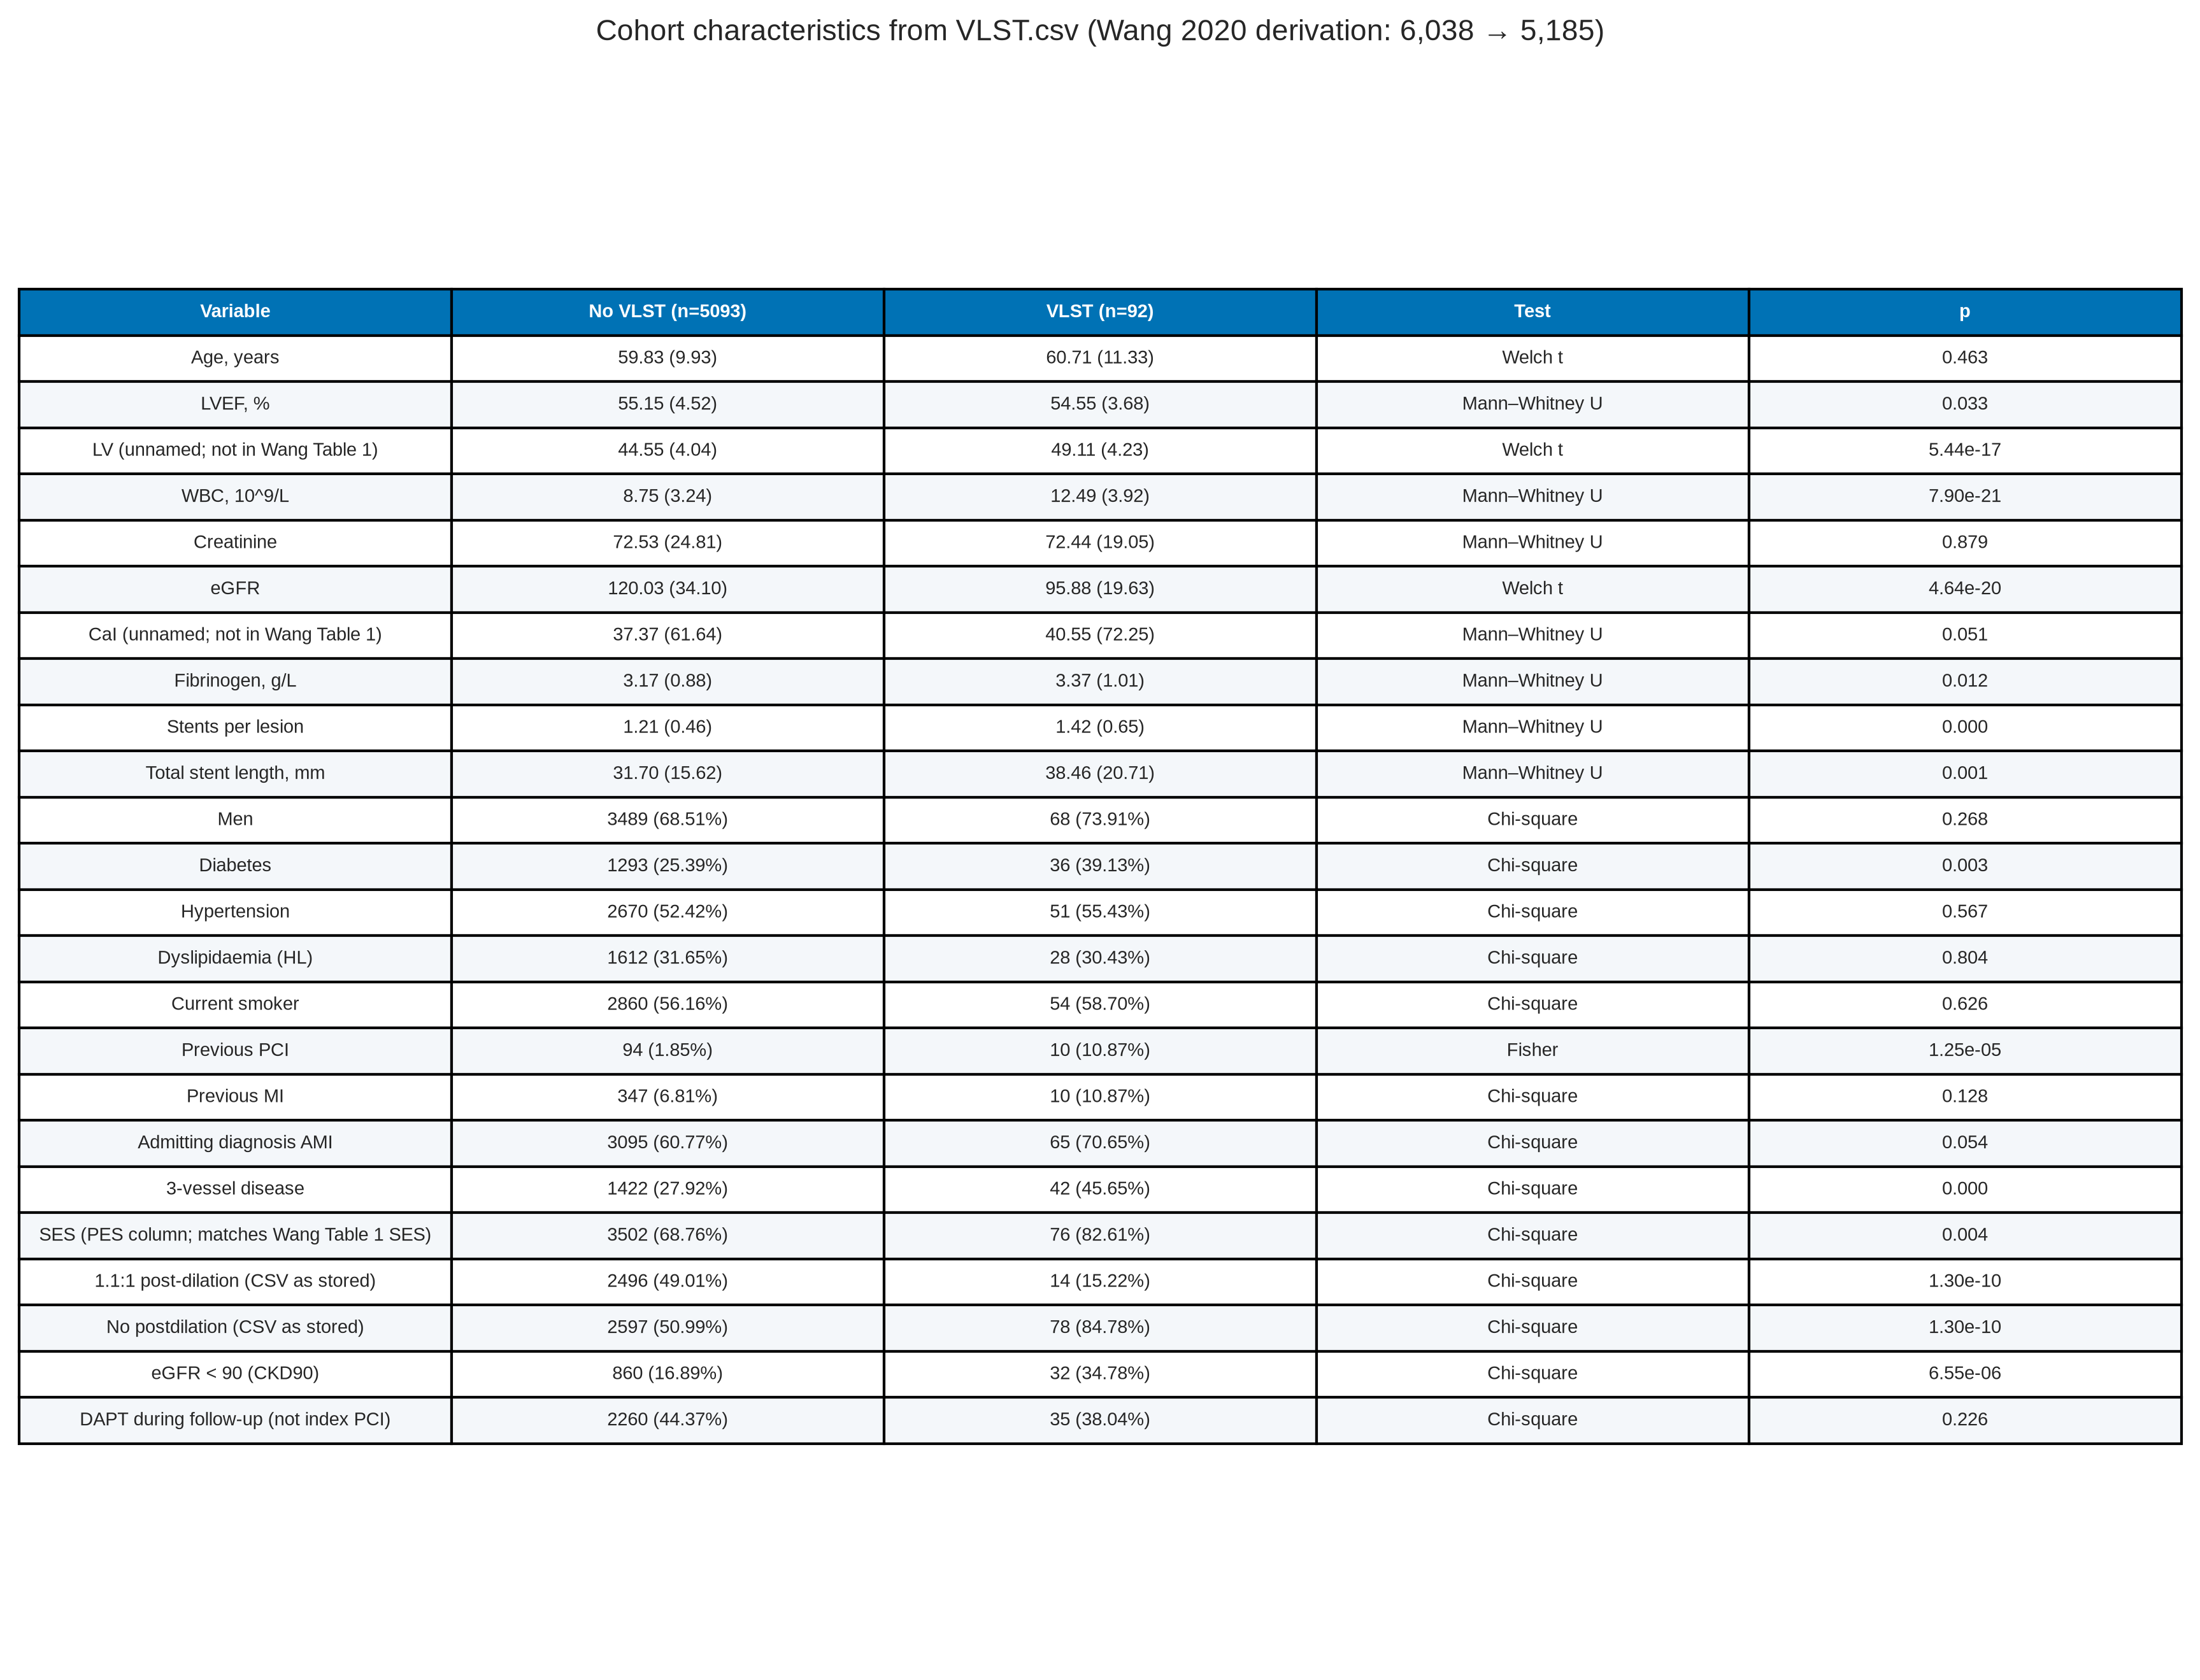
\includegraphics[keepaspectratio,alt={Table 1. Cohort characteristics}]{../paper_results/01_eda/paper_figures/paper_table_c_cohort_characteristics.png}}
\caption{Table 1. Cohort characteristics}
\end{figure}

\begin{center}\rule{0.5\linewidth}{0.5pt}\end{center}

\subsection{4.1 Baseline and anti-leakage
contrast}\label{baseline-and-anti-leakage-contrast}

Same seven classic models, same stratified 70/30 (train 3,629 / test
1,556, seed 42), \texttt{GridSearchCV}
(\texttt{GRID\_SCORING=average\_precision}). \textbf{Not nested CV. Not
TabPFN.} Five flags flip together; SMOTE is ON only in the leaks-on arm.
\textbf{Incentives:} TSSI = mixed time-to-event vs completed follow-up;
WBC = recording-precision / batch marker; unquantized labs =
decimal-grid fingerprint (signature probe AP 0.4270); full-cohort stent
codebook = test-brand leak; train SMOTE = unmatched inflation. Full
protocol: \texttt{paper\_results/anti\_leakage\_protocol.md}. Full
tables: \textbf{Table 2} and
\texttt{leakage\_contrast\_paper\_figures\_and\_tables.md}.

{\def\LTcaptype{none} % do not increment counter
\begin{longtable}[]{@{}
  >{\raggedright\arraybackslash}p{(\linewidth - 4\tabcolsep) * \real{0.3333}}
  >{\raggedright\arraybackslash}p{(\linewidth - 4\tabcolsep) * \real{0.3333}}
  >{\raggedright\arraybackslash}p{(\linewidth - 4\tabcolsep) * \real{0.3333}}@{}}
\toprule\noalign{}
\begin{minipage}[b]{\linewidth}\raggedright
Tag
\end{minipage} & \begin{minipage}[b]{\linewidth}\raggedright
Notebook
\end{minipage} & \begin{minipage}[b]{\linewidth}\raggedright
Flags
\end{minipage} \\
\midrule\noalign{}
\endhead
\bottomrule\noalign{}
\endlastfoot
\textbf{ALL LEAKS ON} & \texttt{baseline\_tssi\_leakage.ipynb} &
\texttt{KEEP\_TSSI=True}, \texttt{DROP\_WBC=False},
\texttt{QUANTIZE\_CLINICAL=False},
\texttt{STENT\_ENCODER\_TRAIN\_ONLY=False}, \texttt{USE\_SMOTE=True} \\
\textbf{ALL LEAKS OFF} & \texttt{baseline\_without\_tssi.ipynb} &
inverse flags, \texttt{USE\_SMOTE=False} \\
\end{longtable}
}

Hold-out PR-AUC (primary ranking metric at prevalence 0.0177); Δ = ON −
OFF:

{\def\LTcaptype{none} % do not increment counter
\begin{longtable}[]{@{}lrrr@{}}
\toprule\noalign{}
Model & ON & OFF & Δ PR-AUC \\
\midrule\noalign{}
\endhead
\bottomrule\noalign{}
\endlastfoot
Logistic regression & 0.9134 & 0.3431 & \textbf{+0.5703} \\
Decision tree & 0.7524 & 0.1378 & \textbf{+0.6146} \\
Random forest & 0.9400 & 0.4874 & \textbf{+0.4526} \\
Gaussian NB & 0.2728 & 0.0564 & \textbf{+0.2163} \\
CatBoost & 0.9599 & 0.4942 & \textbf{+0.4656} \\
XGBoost & 0.9547 & 0.5685 & \textbf{+0.3862} \\
LightGBM & 0.9687 & 0.6675 & \textbf{+0.3011} \\
\end{longtable}
}

Every model's hold-out PR-AUC is higher on ALL LEAKS ON. Inflation
ranges \textbf{+0.30 to +0.61}. LightGBM is the least inflated booster
and still drops by 0.30.

\begin{figure}
\centering
\pandocbounded{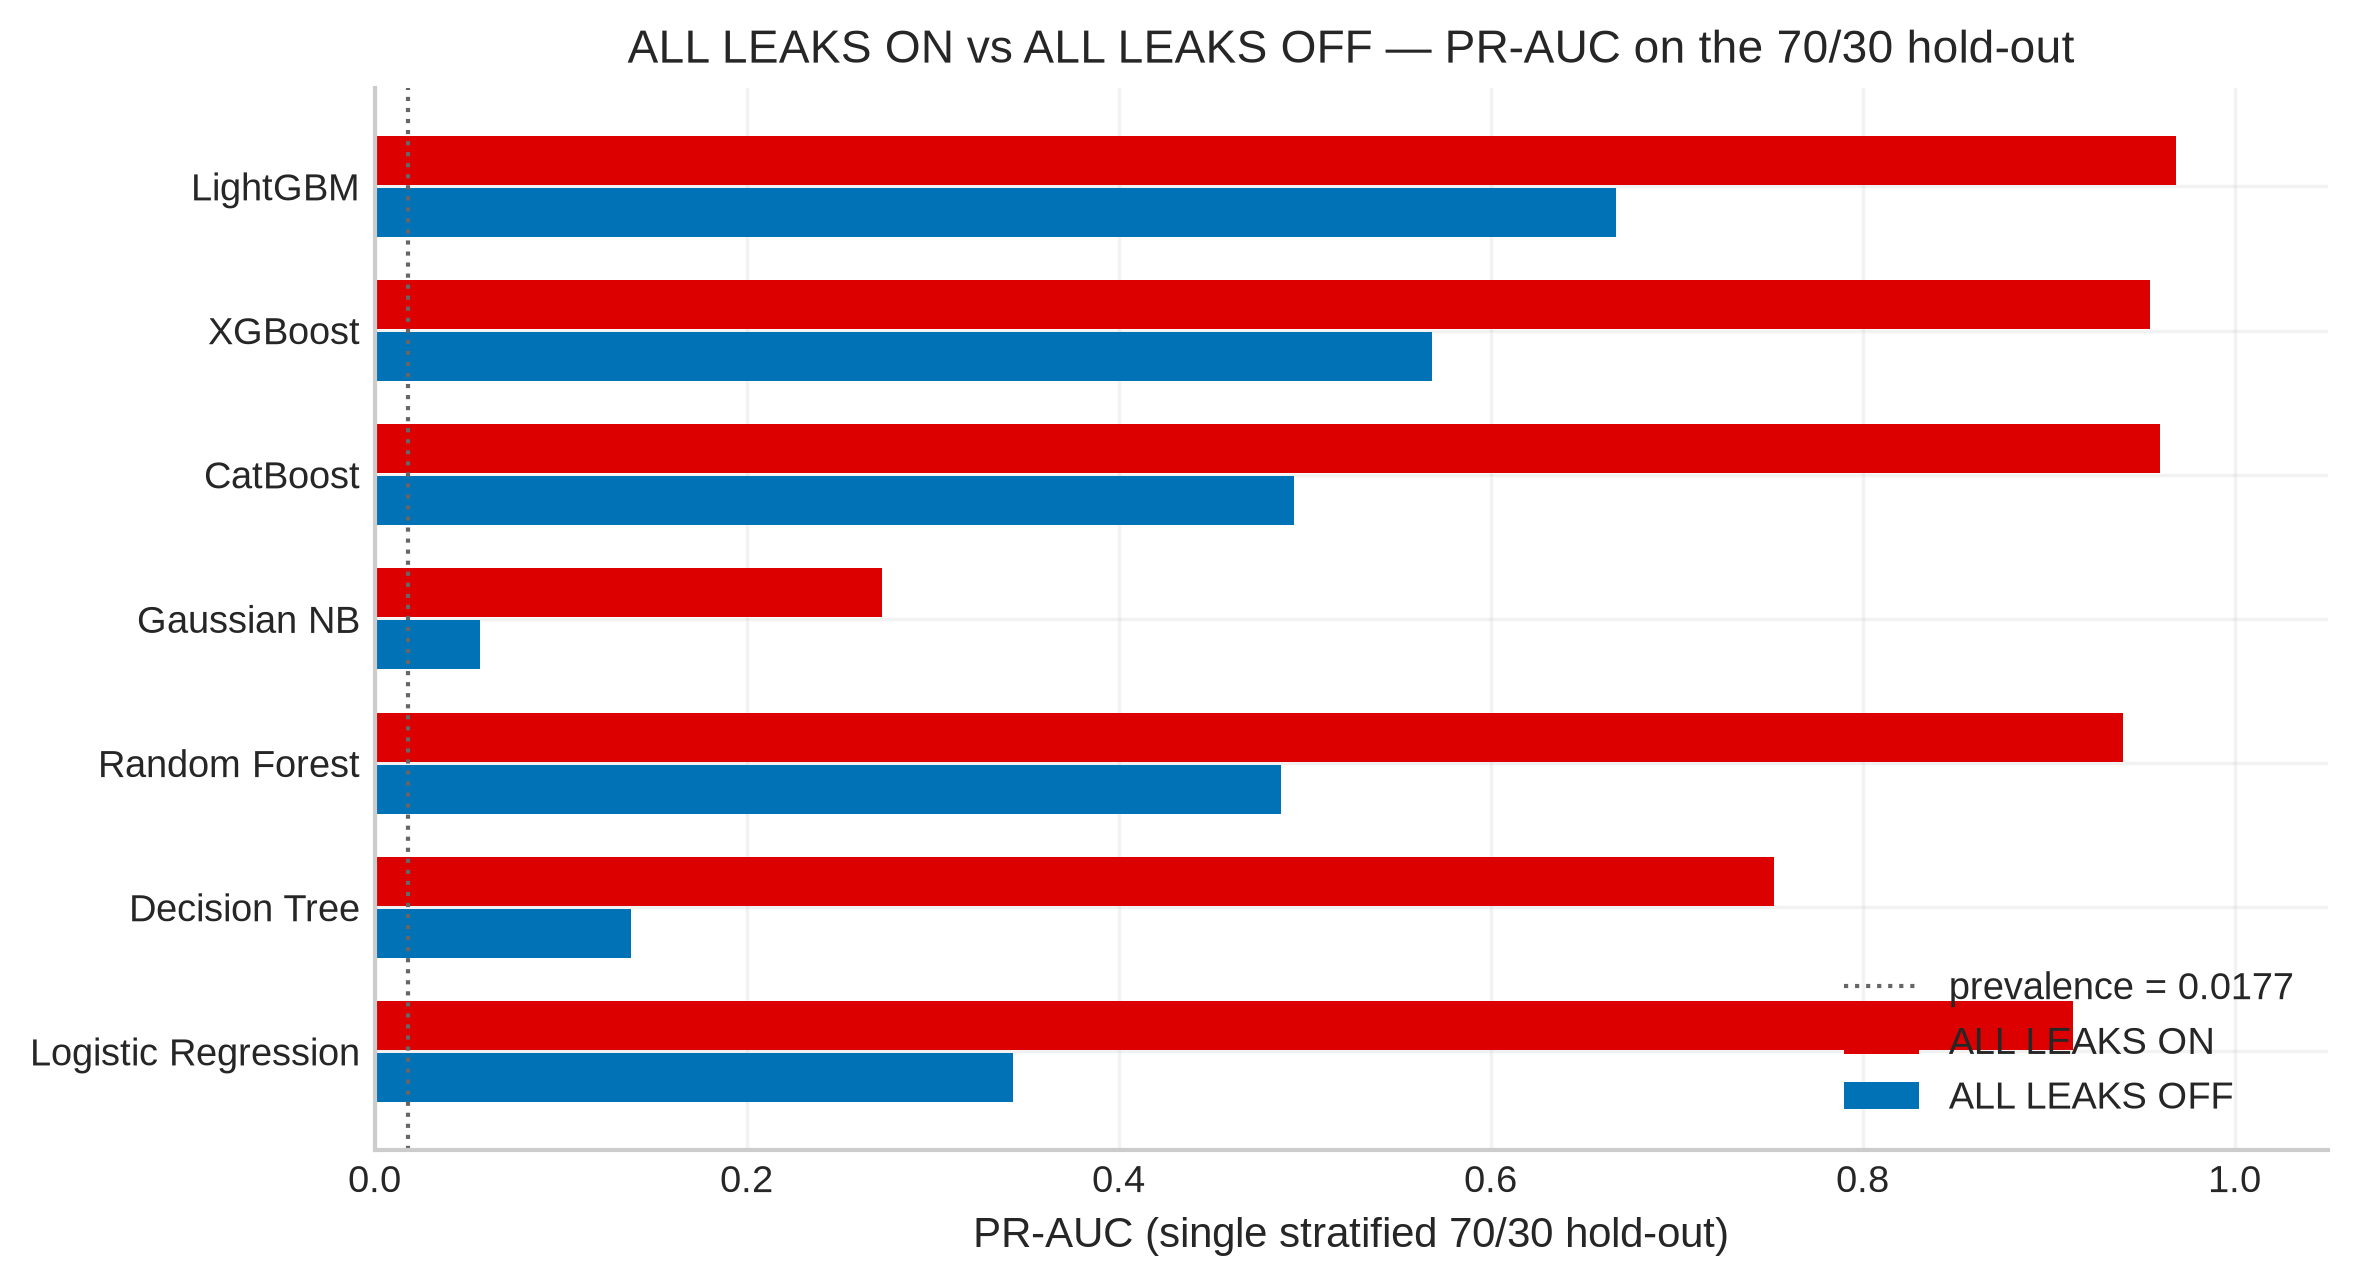
\includegraphics[keepaspectratio,alt={Figure S-TSSI. PR-AUC ALL LEAKS ON vs OFF}]{../paper_results/04_tabpfn_rating/paper_figures/paper_fig_s_tssi_pr_auc.png}}
\caption{Figure S-TSSI. PR-AUC ALL LEAKS ON vs OFF}
\end{figure}

ROC-AUC compression is smaller. \textbf{Dual-label:} Gaussian NB ROC-AUC
is slightly \emph{higher} OFF (0.7493 vs 0.7425) while PR-AUC still
falls (0.2728 → 0.0564). Do not write ``every metric falls.''

At the notebook operating point, random forest F1 on ALL LEAKS OFF is
\textbf{0} (no predicted events) while ROC-AUC remains 0.9287. Boosters
that look near-perfect on ON (F1 0.9231, precision 1.0) drop to F1
0.41--0.55 once leak flags are off. Accuracy stays high except GNB
because 1,528/1,556 hold-out rows are non-events; accuracy is not the
ranking metric.

\textbf{Reading.} A 70/30 GridSearch pipeline that retains TSSI (and
WBC, unquantized labs, a full-cohort stent encoder, and train SMOTE)
\textbf{overstates hold-out ranking on this derivation file}. Nested CV,
Part 2, and Part 5 therefore implement the OFF flags. This subsection
does not transfer to TabPFN. \textbf{ARCHIVED:} LR PR-AUC 0.9575 →
0.5077.

\begin{center}\rule{0.5\linewidth}{0.5pt}\end{center}

\subsection{4.2 Nested ranking: TabPFN checkpoints vs library-default
reference
panel}\label{nested-ranking-tabpfn-checkpoints-vs-library-default-reference-panel}

Dump:
\texttt{Kaggle\_baseline\_plus\_tabpfn\_results/baseline\_plus\_tabpfn\_results/}
(\texttt{tabpfn==9.0.0}, \texttt{tabpfn-client==0.6.0}, Tesla T4, 9
arms). Nested 5×4, seed 42, inner loop = F1 threshold only. Five classic
arms = \textbf{untuned reference panel} (defaults + class weighting;
GridSearch winners \textbf{not} imported). No SMOTE. Leak status for the
entire table: anti-leakage \textbf{ON} (five-flag OFF: IDs+TSSI+WBC
dropped; labs quantized pre-split; \texttt{encode\_stent\_on\_fold}; no
SMOTE). Full numbers: \textbf{Table 3}. Bootstrap 95\% CIs: stratified
resample of stored OOF, \texttt{n\_boot=2000}, seed 42; models not
re-fit.

\textbf{Figure 1.} Nested-CV out-of-fold PR and ROC curves.

\begin{figure}
\centering
\pandocbounded{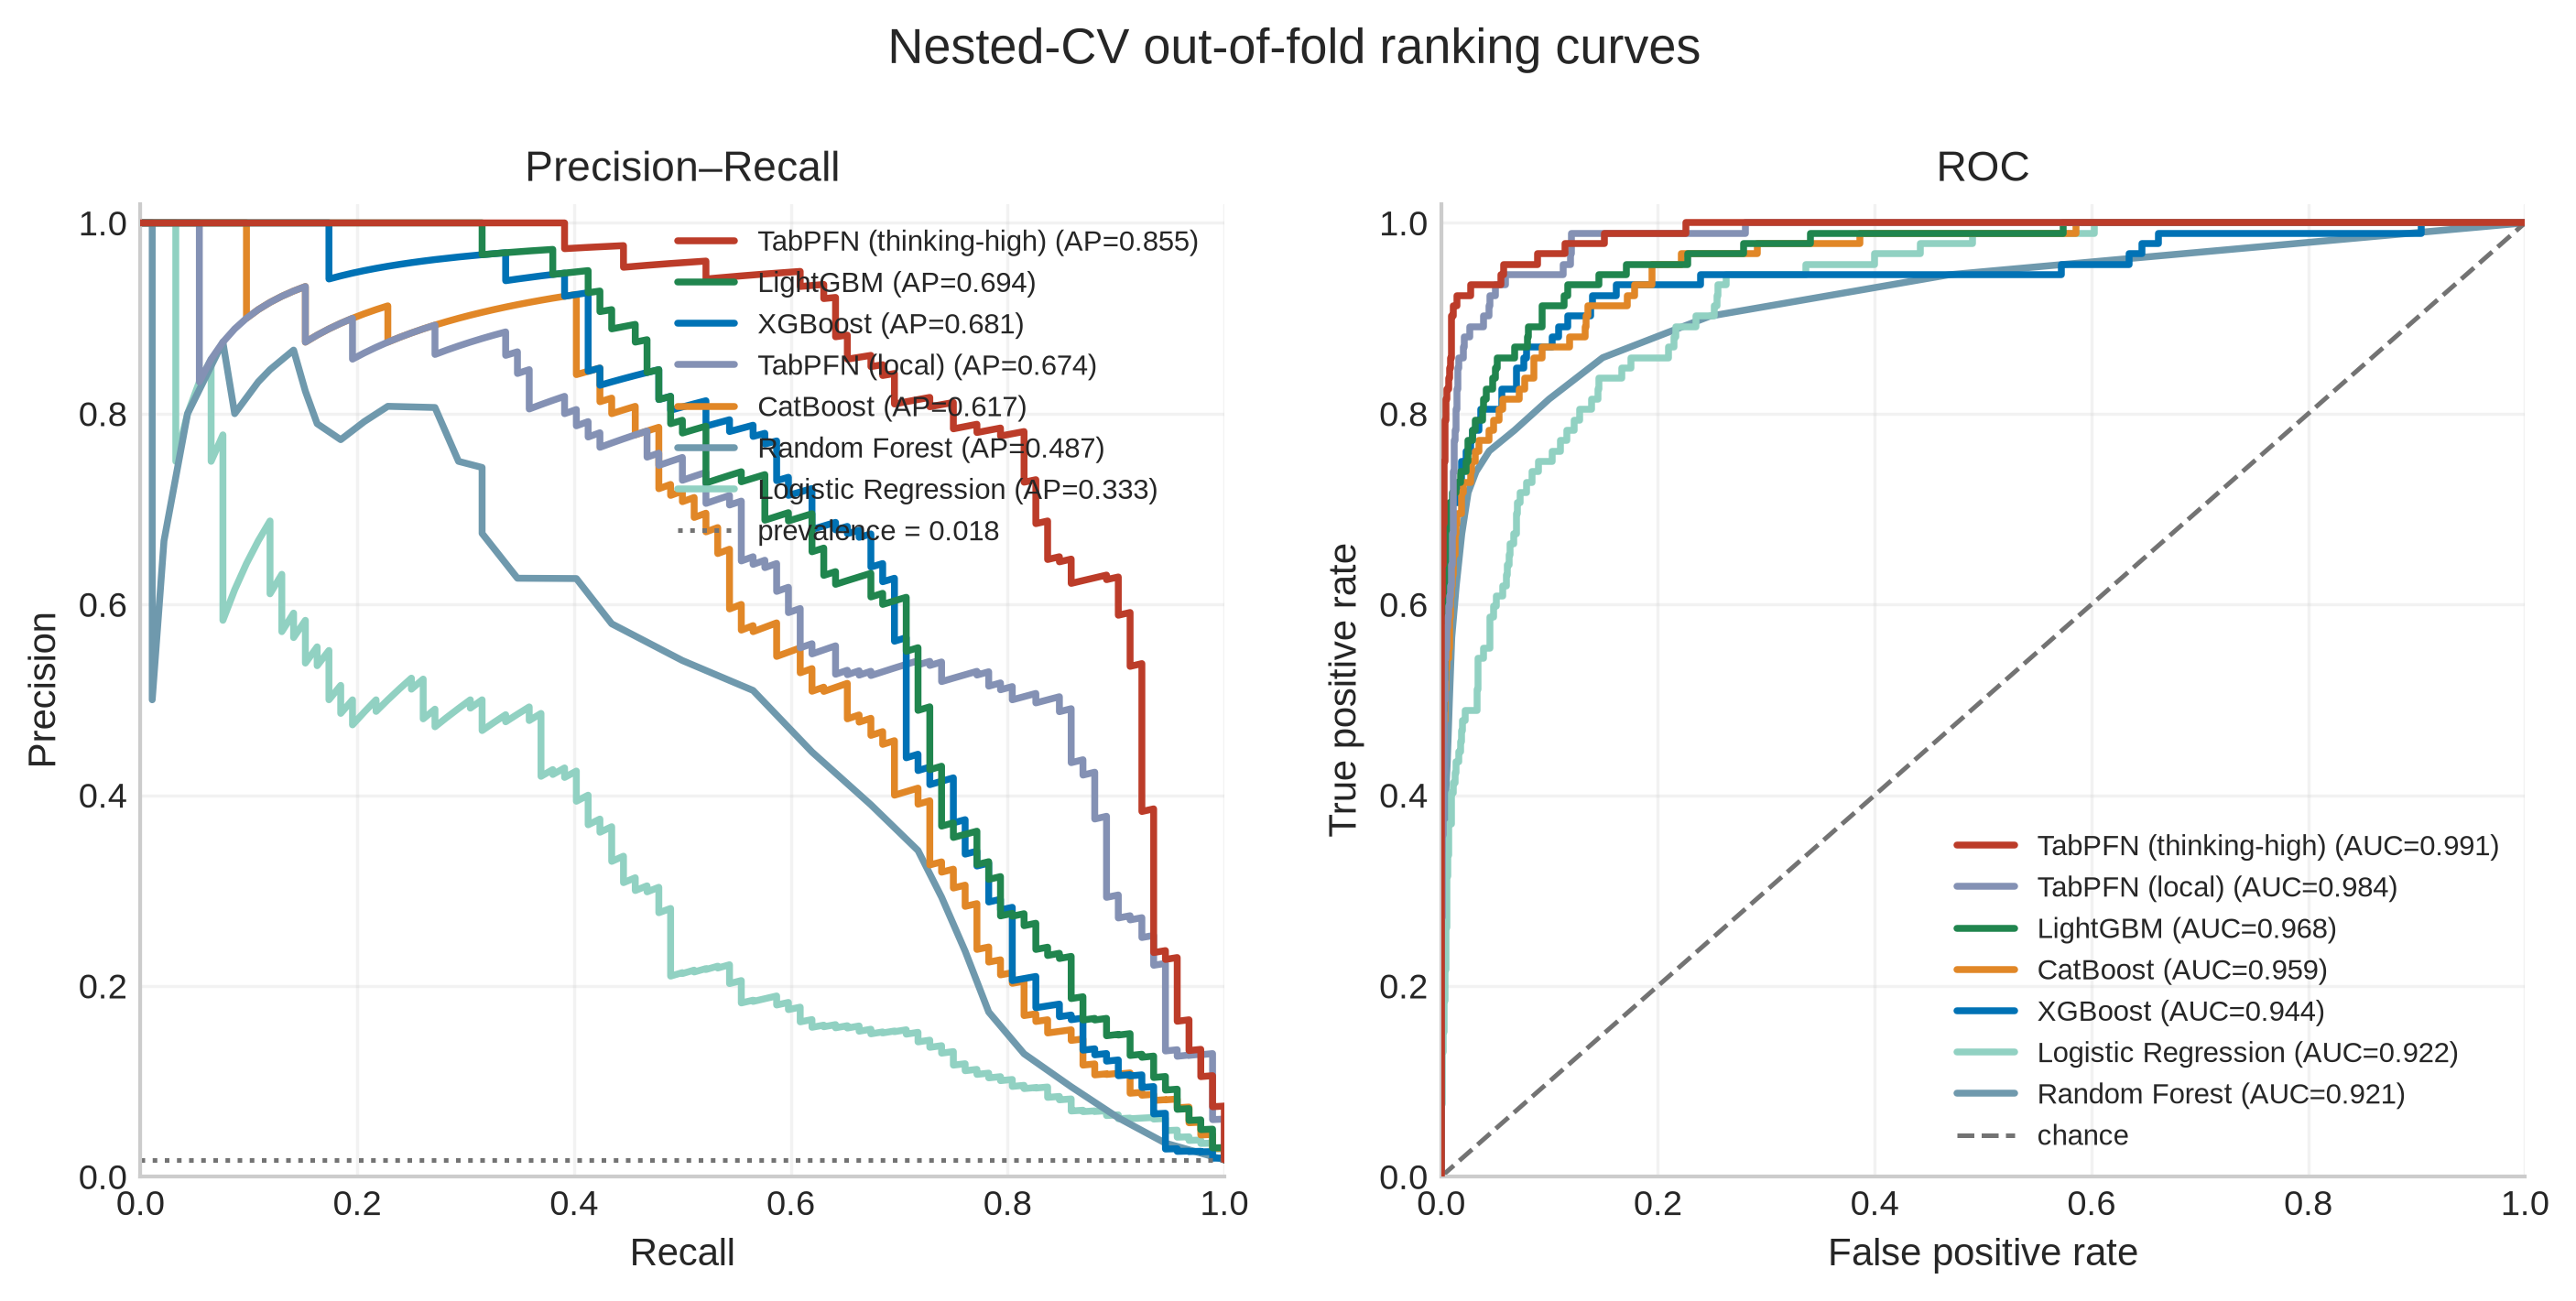
\includegraphics[keepaspectratio,alt={Figure 1. Nested OOF PR and ROC}]{../paper_results/04_tabpfn_rating/paper_figures/paper_fig1_pr_roc_curves.png}}
\caption{Figure 1. Nested OOF PR and ROC}
\end{figure}

Pooled nested OOF ranking (threshold-independent):

{\def\LTcaptype{none} % do not increment counter
\begin{longtable}[]{@{}
  >{\raggedleft\arraybackslash}p{(\linewidth - 12\tabcolsep) * \real{0.1600}}
  >{\raggedright\arraybackslash}p{(\linewidth - 12\tabcolsep) * \real{0.1200}}
  >{\raggedright\arraybackslash}p{(\linewidth - 12\tabcolsep) * \real{0.1200}}
  >{\raggedright\arraybackslash}p{(\linewidth - 12\tabcolsep) * \real{0.1200}}
  >{\raggedleft\arraybackslash}p{(\linewidth - 12\tabcolsep) * \real{0.1600}}
  >{\raggedleft\arraybackslash}p{(\linewidth - 12\tabcolsep) * \real{0.1600}}
  >{\raggedleft\arraybackslash}p{(\linewidth - 12\tabcolsep) * \real{0.1600}}@{}}
\toprule\noalign{}
\begin{minipage}[b]{\linewidth}\raggedleft
Rank
\end{minipage} & \begin{minipage}[b]{\linewidth}\raggedright
Model
\end{minipage} & \begin{minipage}[b]{\linewidth}\raggedright
Checkpoint
\end{minipage} & \begin{minipage}[b]{\linewidth}\raggedright
Thinking
\end{minipage} & \begin{minipage}[b]{\linewidth}\raggedleft
PR-AUC (95\% CI)
\end{minipage} & \begin{minipage}[b]{\linewidth}\raggedleft
ROC-AUC
\end{minipage} & \begin{minipage}[b]{\linewidth}\raggedleft
Brier
\end{minipage} \\
\midrule\noalign{}
\endhead
\bottomrule\noalign{}
\endlastfoot
1 & TabPFN thinking v3.5 & hosted \texttt{v3.5\_default} & thinking-high
& \textbf{0.9212} {[}0.8785, 0.9613{]} & 0.9963 & 0.0047 \\
2 & TabPFN v3.5 & local \texttt{tabpfn-v3.5-20260909.safetensors} &
local & \textbf{0.8957} {[}0.8446, 0.9426{]} & 0.9916 & 0.0048 \\
3 & TabPFN thinking v3 & hosted \texttt{v3\_default} & thinking-high &
0.8319 {[}0.7626, 0.8945{]} & 0.9834 & 0.0066 \\
4 & TabPFN v3 & local v3 ckpt & local & 0.7150 {[}0.6260, 0.8074{]} &
0.9731 & 0.0099 \\
5 & XGBoost & n/a & n/a & 0.6322 {[}0.5331, 0.7247{]} & 0.9374 &
0.0100 \\
6 & LightGBM & n/a & n/a & 0.6271 {[}0.5313, 0.7202{]} & 0.9444 &
0.0106 \\
7 & CatBoost & n/a & n/a & 0.5707 {[}0.4750, 0.6729{]} & 0.9404 &
0.0108 \\
8 & Random forest & n/a & n/a & 0.3506 {[}0.2660, 0.4633{]} & 0.8883 &
0.0150 \\
9 & Logistic regression & n/a & n/a & 0.2596 {[}0.1834, 0.3588{]} &
0.8651 & 0.0788 \\
\end{longtable}
}

\textbf{TabPFN vs library-default reference panel.} Highest
default-classic PR-AUC is XGBoost 0.6322, then LightGBM 0.6271. These
are not GridSearch winners. Paired bootstrap Δ PR-AUC: thinking v3.5 −
LightGBM \textbf{0.2941} (0.2071--0.3805), P(Δ ≤ 0) = 0/2000; TabPFN
v3.5 − LightGBM \textbf{0.2686} (0.1822--0.3559), P = 0/2000; thinking
v3.5 − XGBoost \textbf{0.2891} (0.2038--0.3791), P = 0/2000. The Δ is a
contrast of stored OOF vectors, not evidence that tuned boosting would
lose by the same margin.

\textbf{v3 vs v3.5 (same thinking status).} Local: 0.8957 vs 0.7150.
Thinking: 0.9212 vs 0.8319.

\textbf{Thinking vs local (same checkpoint family).} v3.5: 0.9212 vs
0.8957. v3: 0.8319 vs 0.7150. Thinking v3.5 is \textbf{not} higher than
local v3.5 in every fold (fold 1: local 0.9365 vs thinking 0.8802). Fold
PR-AUC thinking v3.5: 0.8802, 0.9078, 0.9434, 0.9858, 0.8961.

\textbf{Honest nested operating points (inner-fold F1 thresholds ---
quote these, not pooled cuts).} Thinking v3.5: \emph{t} 0.318 ± 0.059;
5083/10/15/77; sensitivity \textbf{0.8370}; precision \textbf{0.8851};
F1 \textbf{0.8603}. TabPFN v3.5: 5082/11/20/72; sensitivity
\textbf{0.7826}; precision \textbf{0.8675}; F1 \textbf{0.8229}. XGBoost:
sensitivity 0.5217; F1 0.5818. LightGBM: sensitivity \textbf{0.5870}; F1
\textbf{0.5902}. ROC-AUC CIs (thinking v3.5 \textbf{0.9963} {[}0.9932,
0.9986{]}; TabPFN v3.5 \textbf{0.9916} {[}0.9828, 0.9978{]}). Nested-CV
discrimination on the derivation file is not external validation.

\begin{figure}
\centering
\pandocbounded{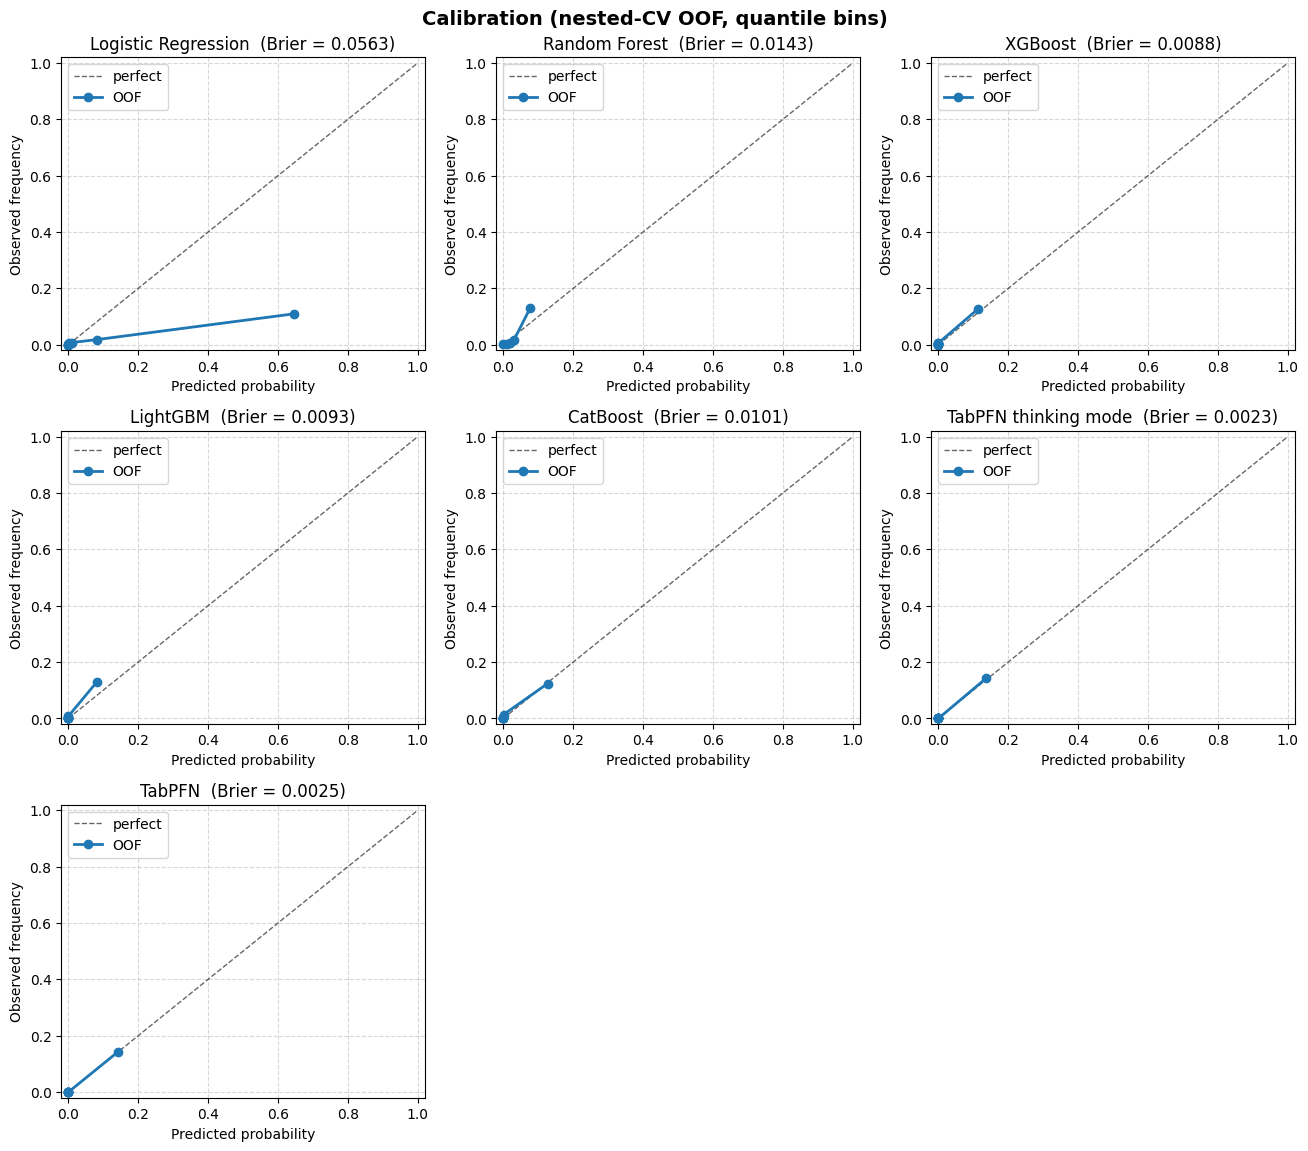
\includegraphics[keepaspectratio,alt={Figure 2. Nested calibration}]{../paper_results/04_tabpfn_rating/paper_figures/paper_fig2_calibration_curves.png}}
\caption{Figure 2. Nested calibration}
\end{figure}

\textbf{Wang integer score (frozen comparator, not a nested arm).}
Full-cohort ROC-AUC \textbf{0.8013}, PR-AUC \textbf{0.1032}. SES points
use \texttt{PES}; four post-dilation points use
\texttt{No\ postdilation} = 1. Flipped encoding ROC-AUC \textbf{0.5084}
is rejected.

\begin{center}\rule{0.5\linewidth}{0.5pt}\end{center}

\subsection{4.3 Feature-selection stability across 8
seeds}\label{feature-selection-stability-across-8-seeds}

Forward sequential feature selection (keep 10 of 80, 5-fold CV, average
precision) repeated over \textbf{8/8 shuffled seeds} on the
\textbf{train} split (n = 3,629), local TabPFN v3.5,
\texttt{FS\_THINKING\_MODE=False}, ALL LEAKS OFF (same quantization +
train-only stent codebook as nested CV). \textbf{Table 4.} Selected in
\textbf{8/8}: \texttt{CaI}, \texttt{LV}, \texttt{eGFR}. Selected in 7/8:
\texttt{Cre}, \texttt{HbA1c}. Selected in 6/8: \texttt{Age}. Selected in
5/8: \texttt{LVEF}. Selected in 4/8 (0.5 cutoff):
\texttt{1.1:1Post\ dilation}. \texttt{WBC} is not a column. A 10-seed
plan was not finished; \textbf{3/10 provisional} tables are archived and
are not this result.

\begin{figure}
\centering
\pandocbounded{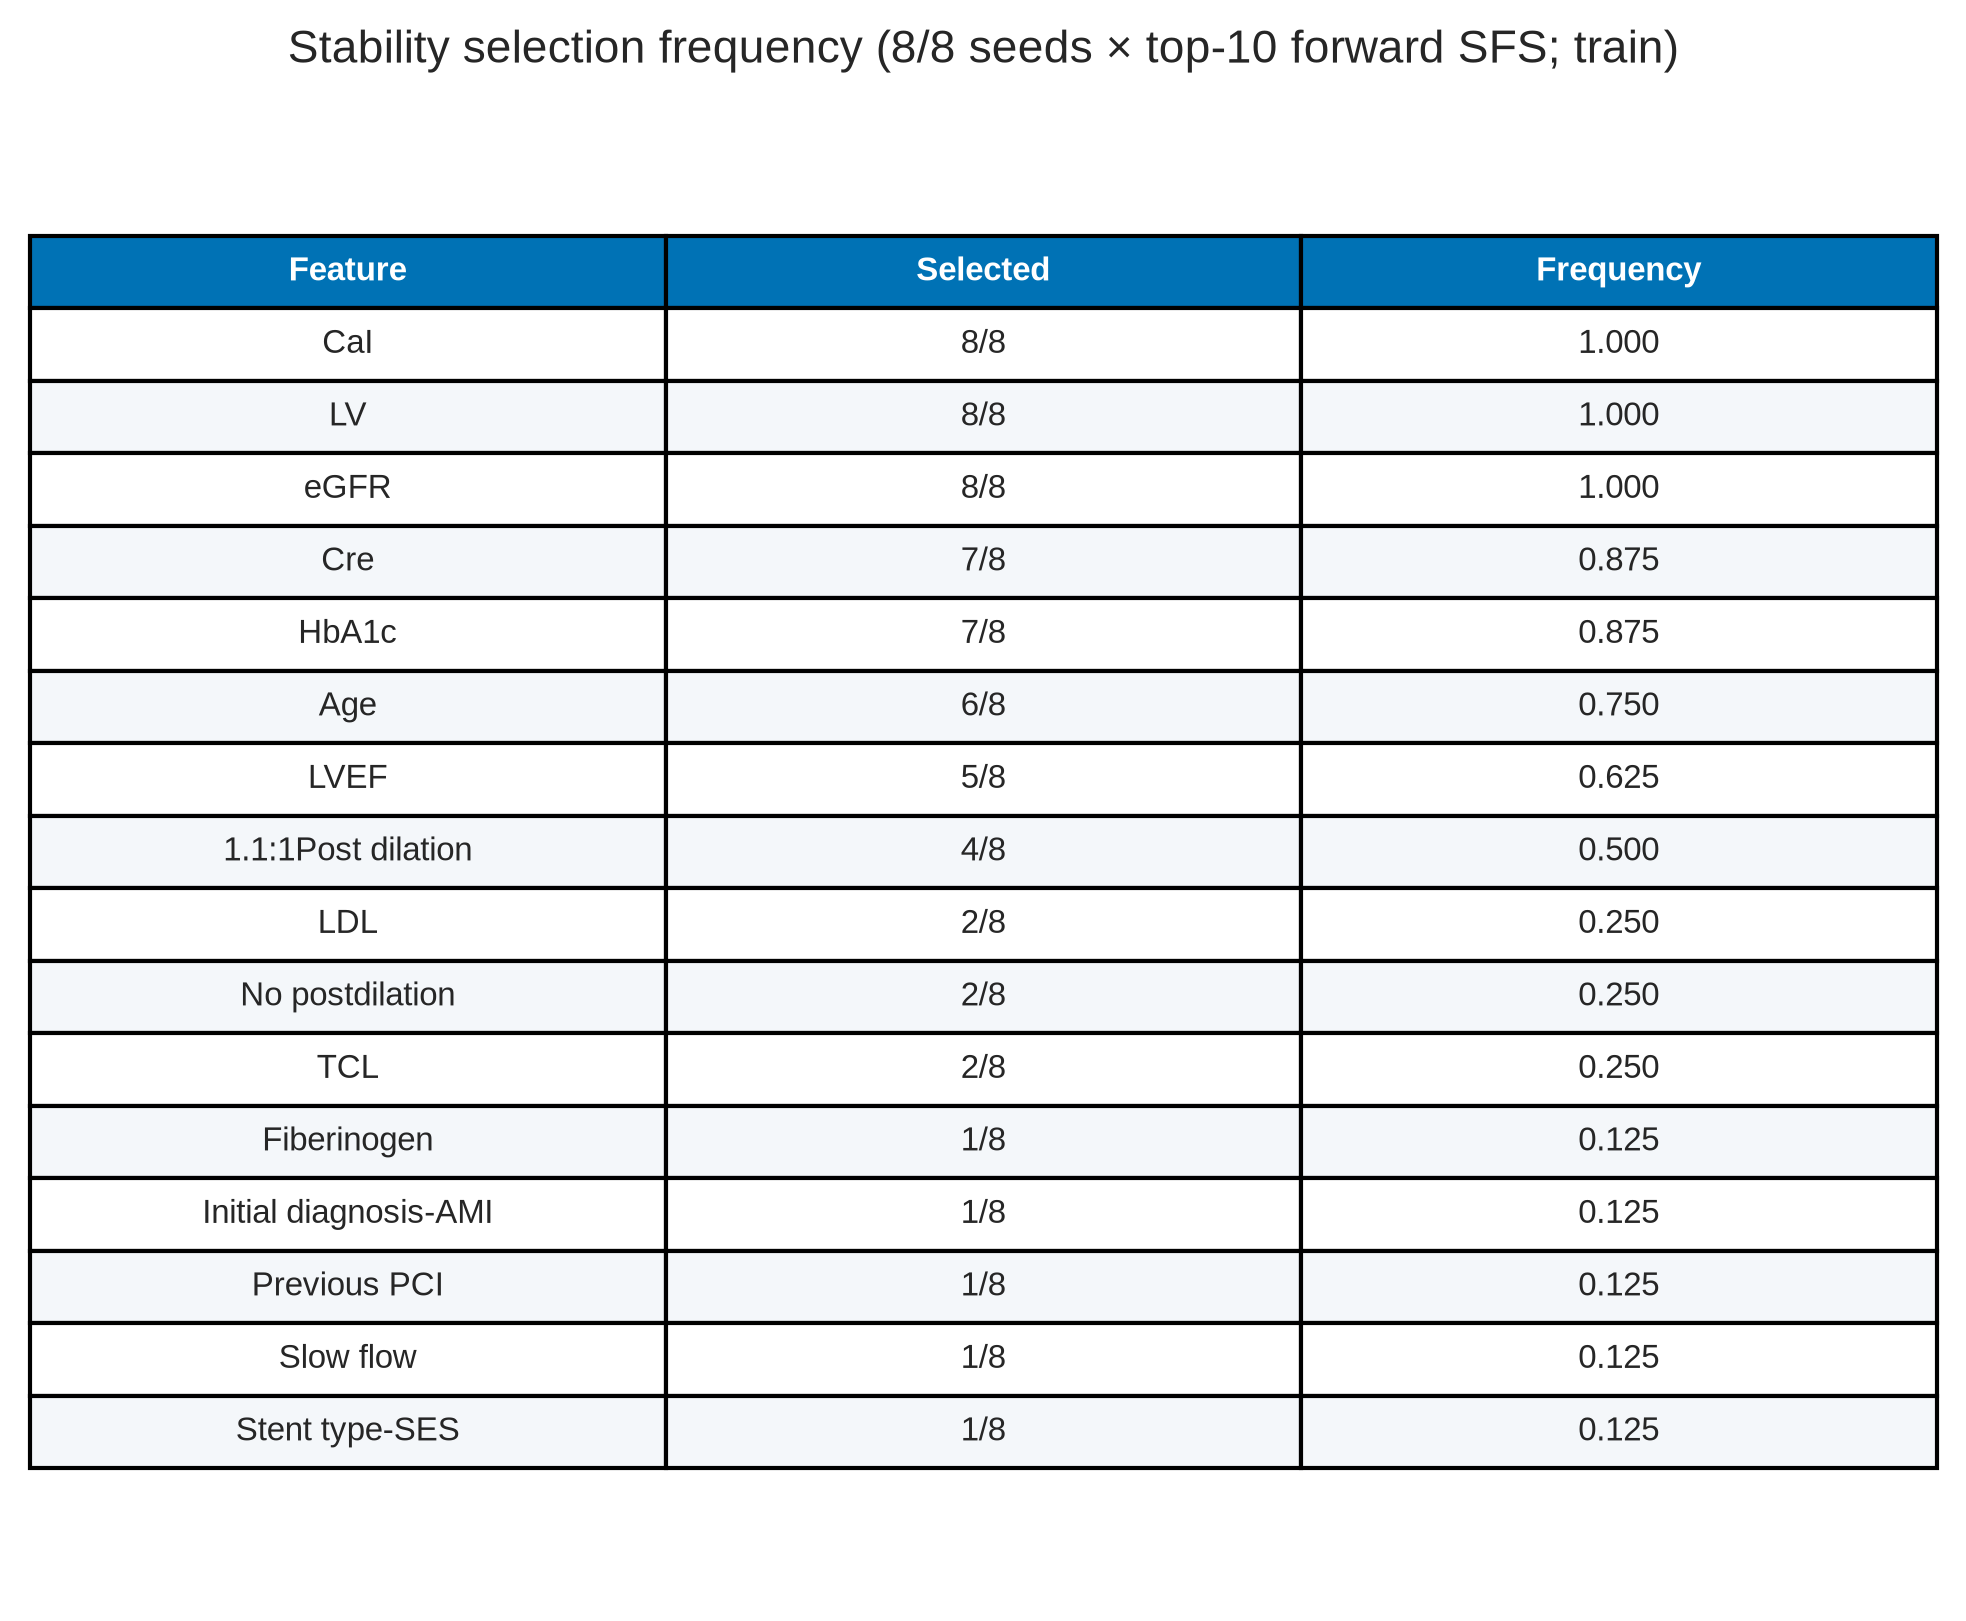
\includegraphics[keepaspectratio,alt={Table 4. SFS stability (8/8 seeds)}]{../paper_results/05_tabpfn_interpretability/paper_figures/paper_table2_stability.png}}
\caption{Table 4. SFS stability (8/8 seeds)}
\end{figure}

Train mutual information (top 5 of 80): CaI 0.020536, LV 0.012818, eGFR
0.009424, LDL 0.009367, HbA1c 0.007328. \texttt{Cre} train MI is
0.000338 (rank 50 of 80). These catalogues are \textbf{attribution}, not
a nested-CV feature mask.

Classic-selector overlap (Part 2/3, anti-leak 19-Sep dump, ML consensus
n = 10 vs FDR-20): intersection
\texttt{\{Clopidogrel,\ HbA1c,\ LV,\ No\ postdilation,\ eGFR\}}; Jaccard
\textbf{5/25 = 0.20}. Dual-label: \texttt{WBC} is FDR-only.

\begin{center}\rule{0.5\linewidth}{0.5pt}\end{center}

\subsection{\texorpdfstring{4.4 Feature attribution and interactions
(SHAP, \emph{k}-SII,
PDP)}{4.4 Feature attribution and interactions (SHAP, k-SII, PDP)}}\label{feature-attribution-and-interactions-shap-k-sii-pdp}

Fit on train; SHAP explains \textbf{all 1,556 held-out rows} (client
thinking-high intended constructor). Mean(\textbar SHAP\textbar) top 4
of 80: \textbf{eGFR 1.2288}, \textbf{CaI 1.0867}, \textbf{Cre 0.8093},
\textbf{LV 0.4828}. \texttt{WBC} is absent. Do not call this 15+15 or
global SHAP on 5,185.

\begin{figure}
\centering
\pandocbounded{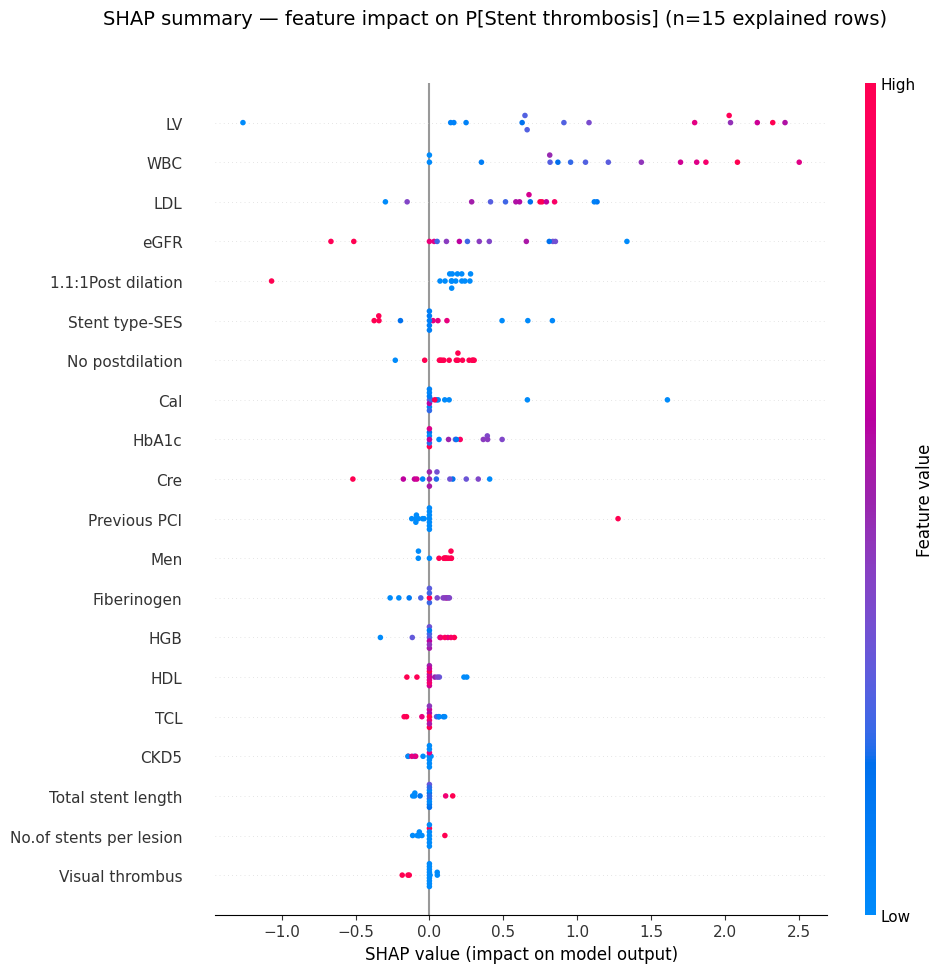
\includegraphics[keepaspectratio,alt={Figure. SHAP summary (held-out)}]{../paper_results/05_tabpfn_interpretability/paper_figures/paper_fig3_shap_summary.png}}
\caption{Figure. SHAP summary (held-out)}
\end{figure}

\begin{figure}
\centering
\pandocbounded{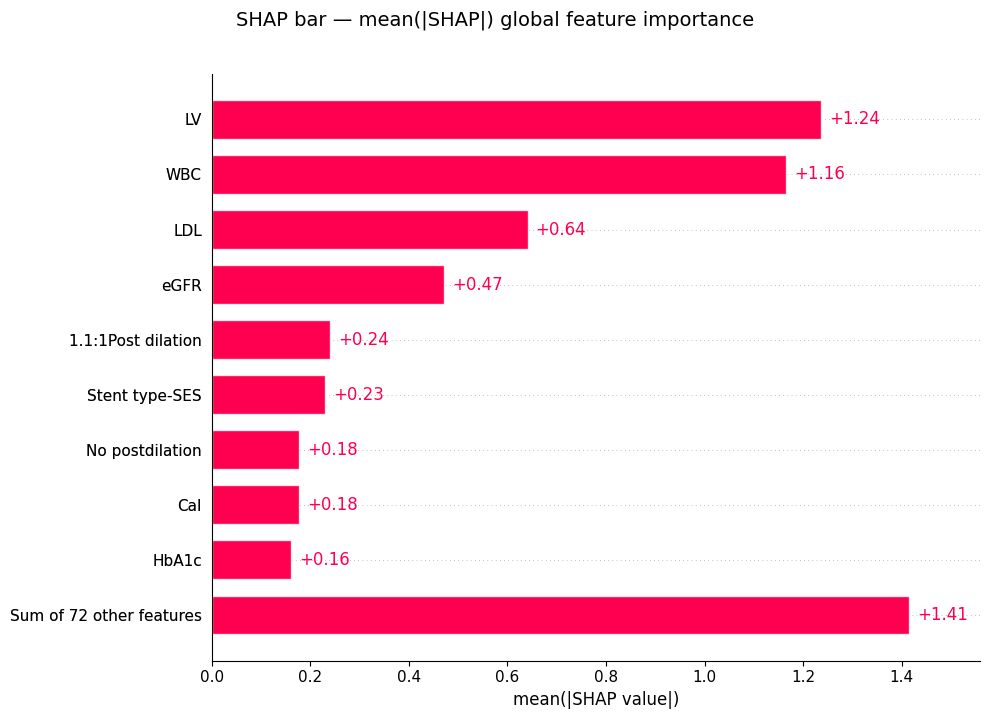
\includegraphics[keepaspectratio,alt={Figure. Mean \textbar SHAP\textbar{} bar}]{../paper_results/05_tabpfn_interpretability/paper_figures/paper_fig5_shap_bar.png}}
\caption{Figure. Mean \textbar SHAP\textbar{} bar}
\end{figure}

Borda consensus after merging held-out SHAP into the fs dump:
\textbf{CaI, eGFR, LV} are 3/3 (also HbA1c and
\texttt{1.1:1Post\ dilation} at the 0.5 SFS cutoff).

\textbf{PDP} (local TabPFN, empirical prior, \textbf{train} n = 3,629).
Y-axis near prevalence (\textasciitilde0.018). \textbf{Not} nested-CV
risk. Largest binary \textbar Δ\textbar: \texttt{Previous\ PCI} 0.017711
→ 0.019006 (Δ \textbf{+0.001294}). \texttt{1.1:1Post\ dilation} Δ
\textbf{−0.000094}. A negative Δ is a lower modelled probability of
recorded VLST, not a treatment benefit.

\begin{figure}
\centering
\pandocbounded{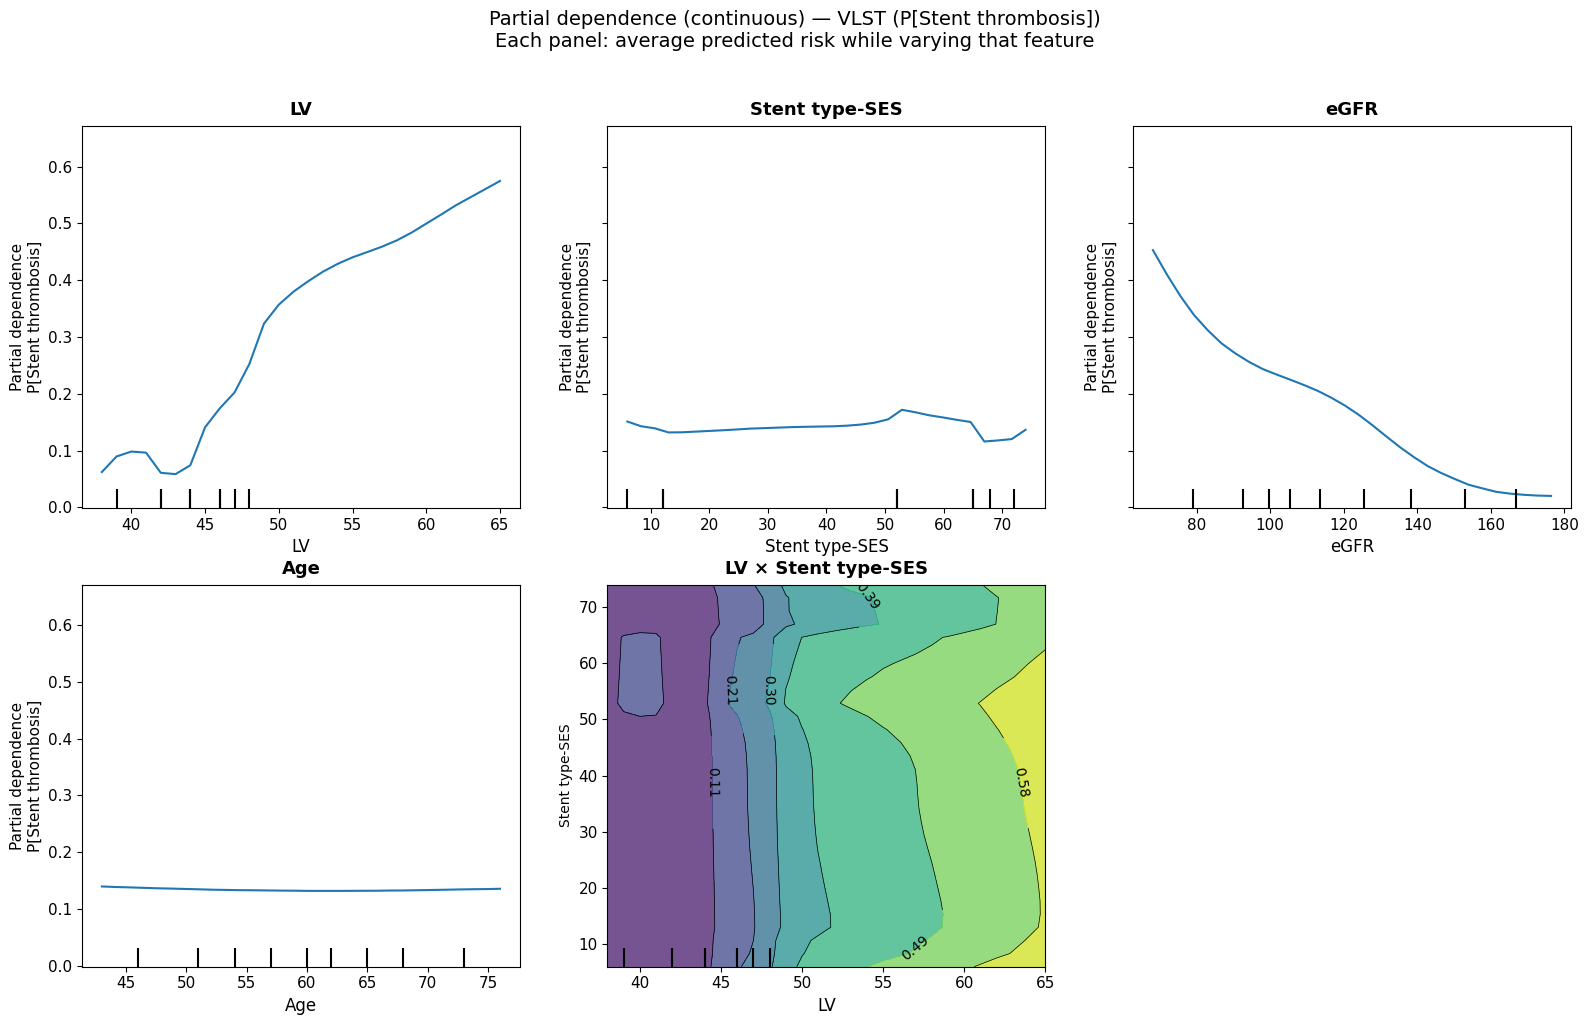
\includegraphics[keepaspectratio,alt={Figure. Continuous PDP (train, empirical prior)}]{../paper_results/05_tabpfn_interpretability/paper_figures/paper_fig1_pdp_continuous.png}}
\caption{Figure. Continuous PDP (train, empirical prior)}
\end{figure}

\begin{figure}
\centering
\pandocbounded{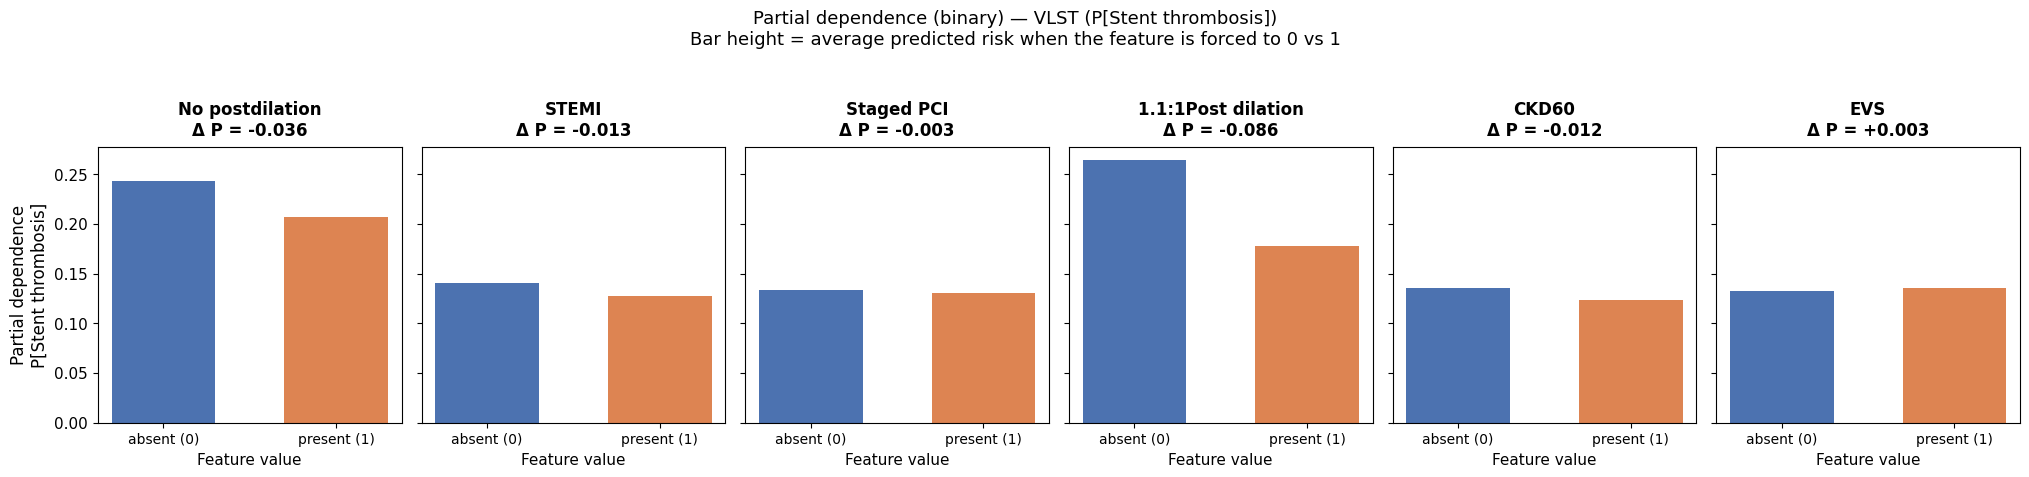
\includegraphics[keepaspectratio,alt={Figure. Binary PDP}]{../paper_results/05_tabpfn_interpretability/paper_figures/paper_fig2_pdp_binary.png}}
\caption{Figure. Binary PDP}
\end{figure}

\textbf{\emph{k}-SII / waterfall} use one held-out VLST=1 row (cohort
\textbf{5176}, budget 256). They illustrate how TabPFN combines features
\textbf{for that patient}; they are not a cohort interaction screen.

\begin{figure}
\centering
\pandocbounded{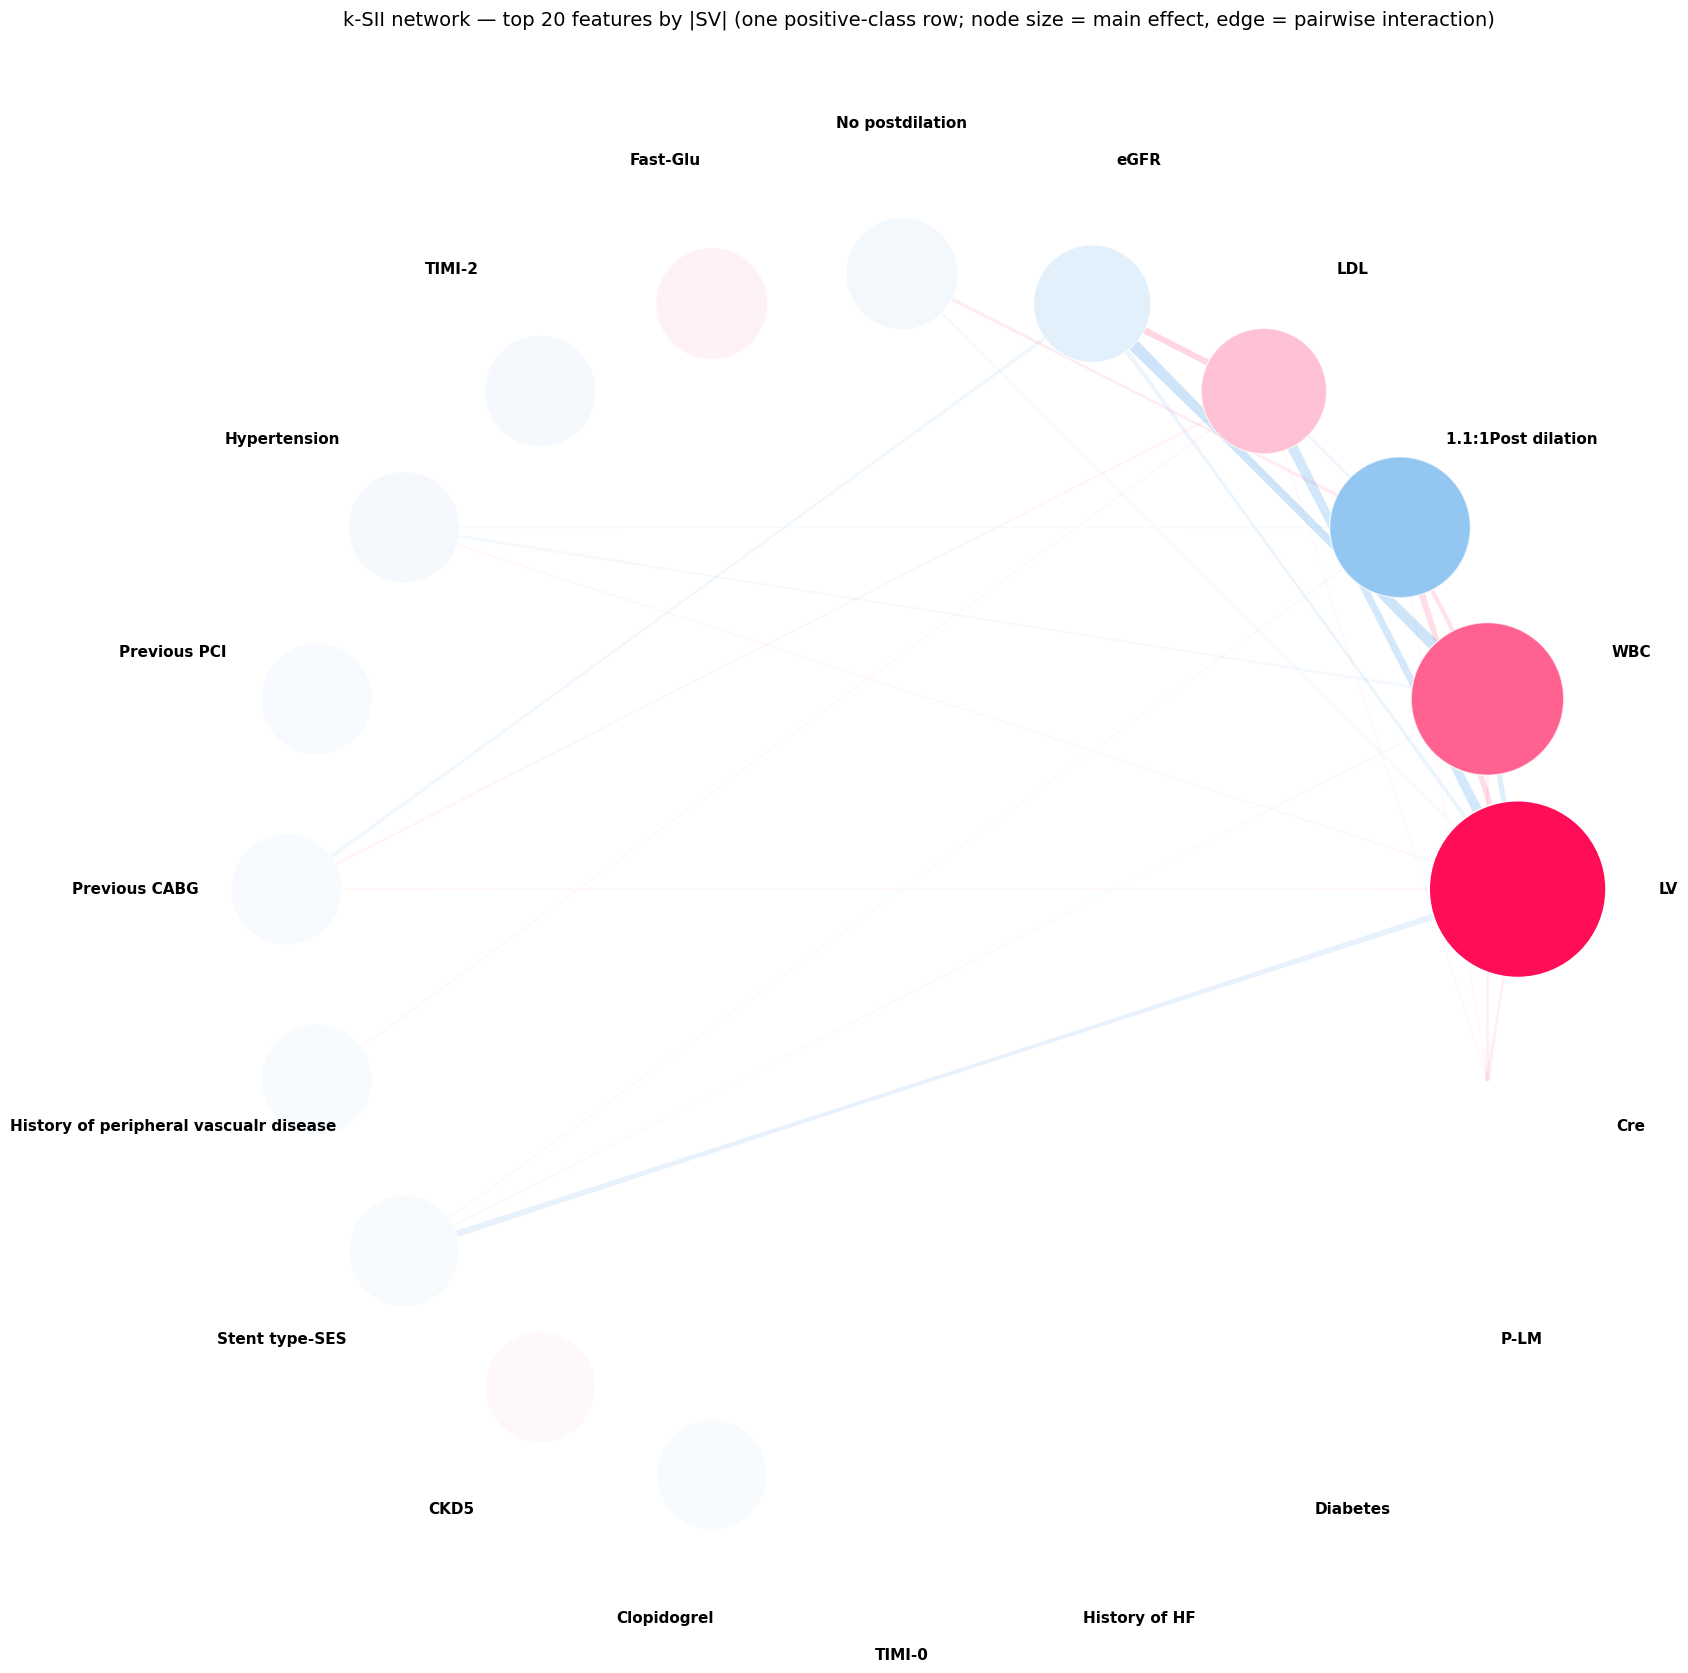
\includegraphics[keepaspectratio,alt={Figure. k-SII network (row 5176)}]{../paper_results/05_tabpfn_interpretability/paper_figures/paper_fig8_ksii_network.png}}
\caption{Figure. k-SII network (row 5176)}
\end{figure}

\begin{figure}
\centering
\pandocbounded{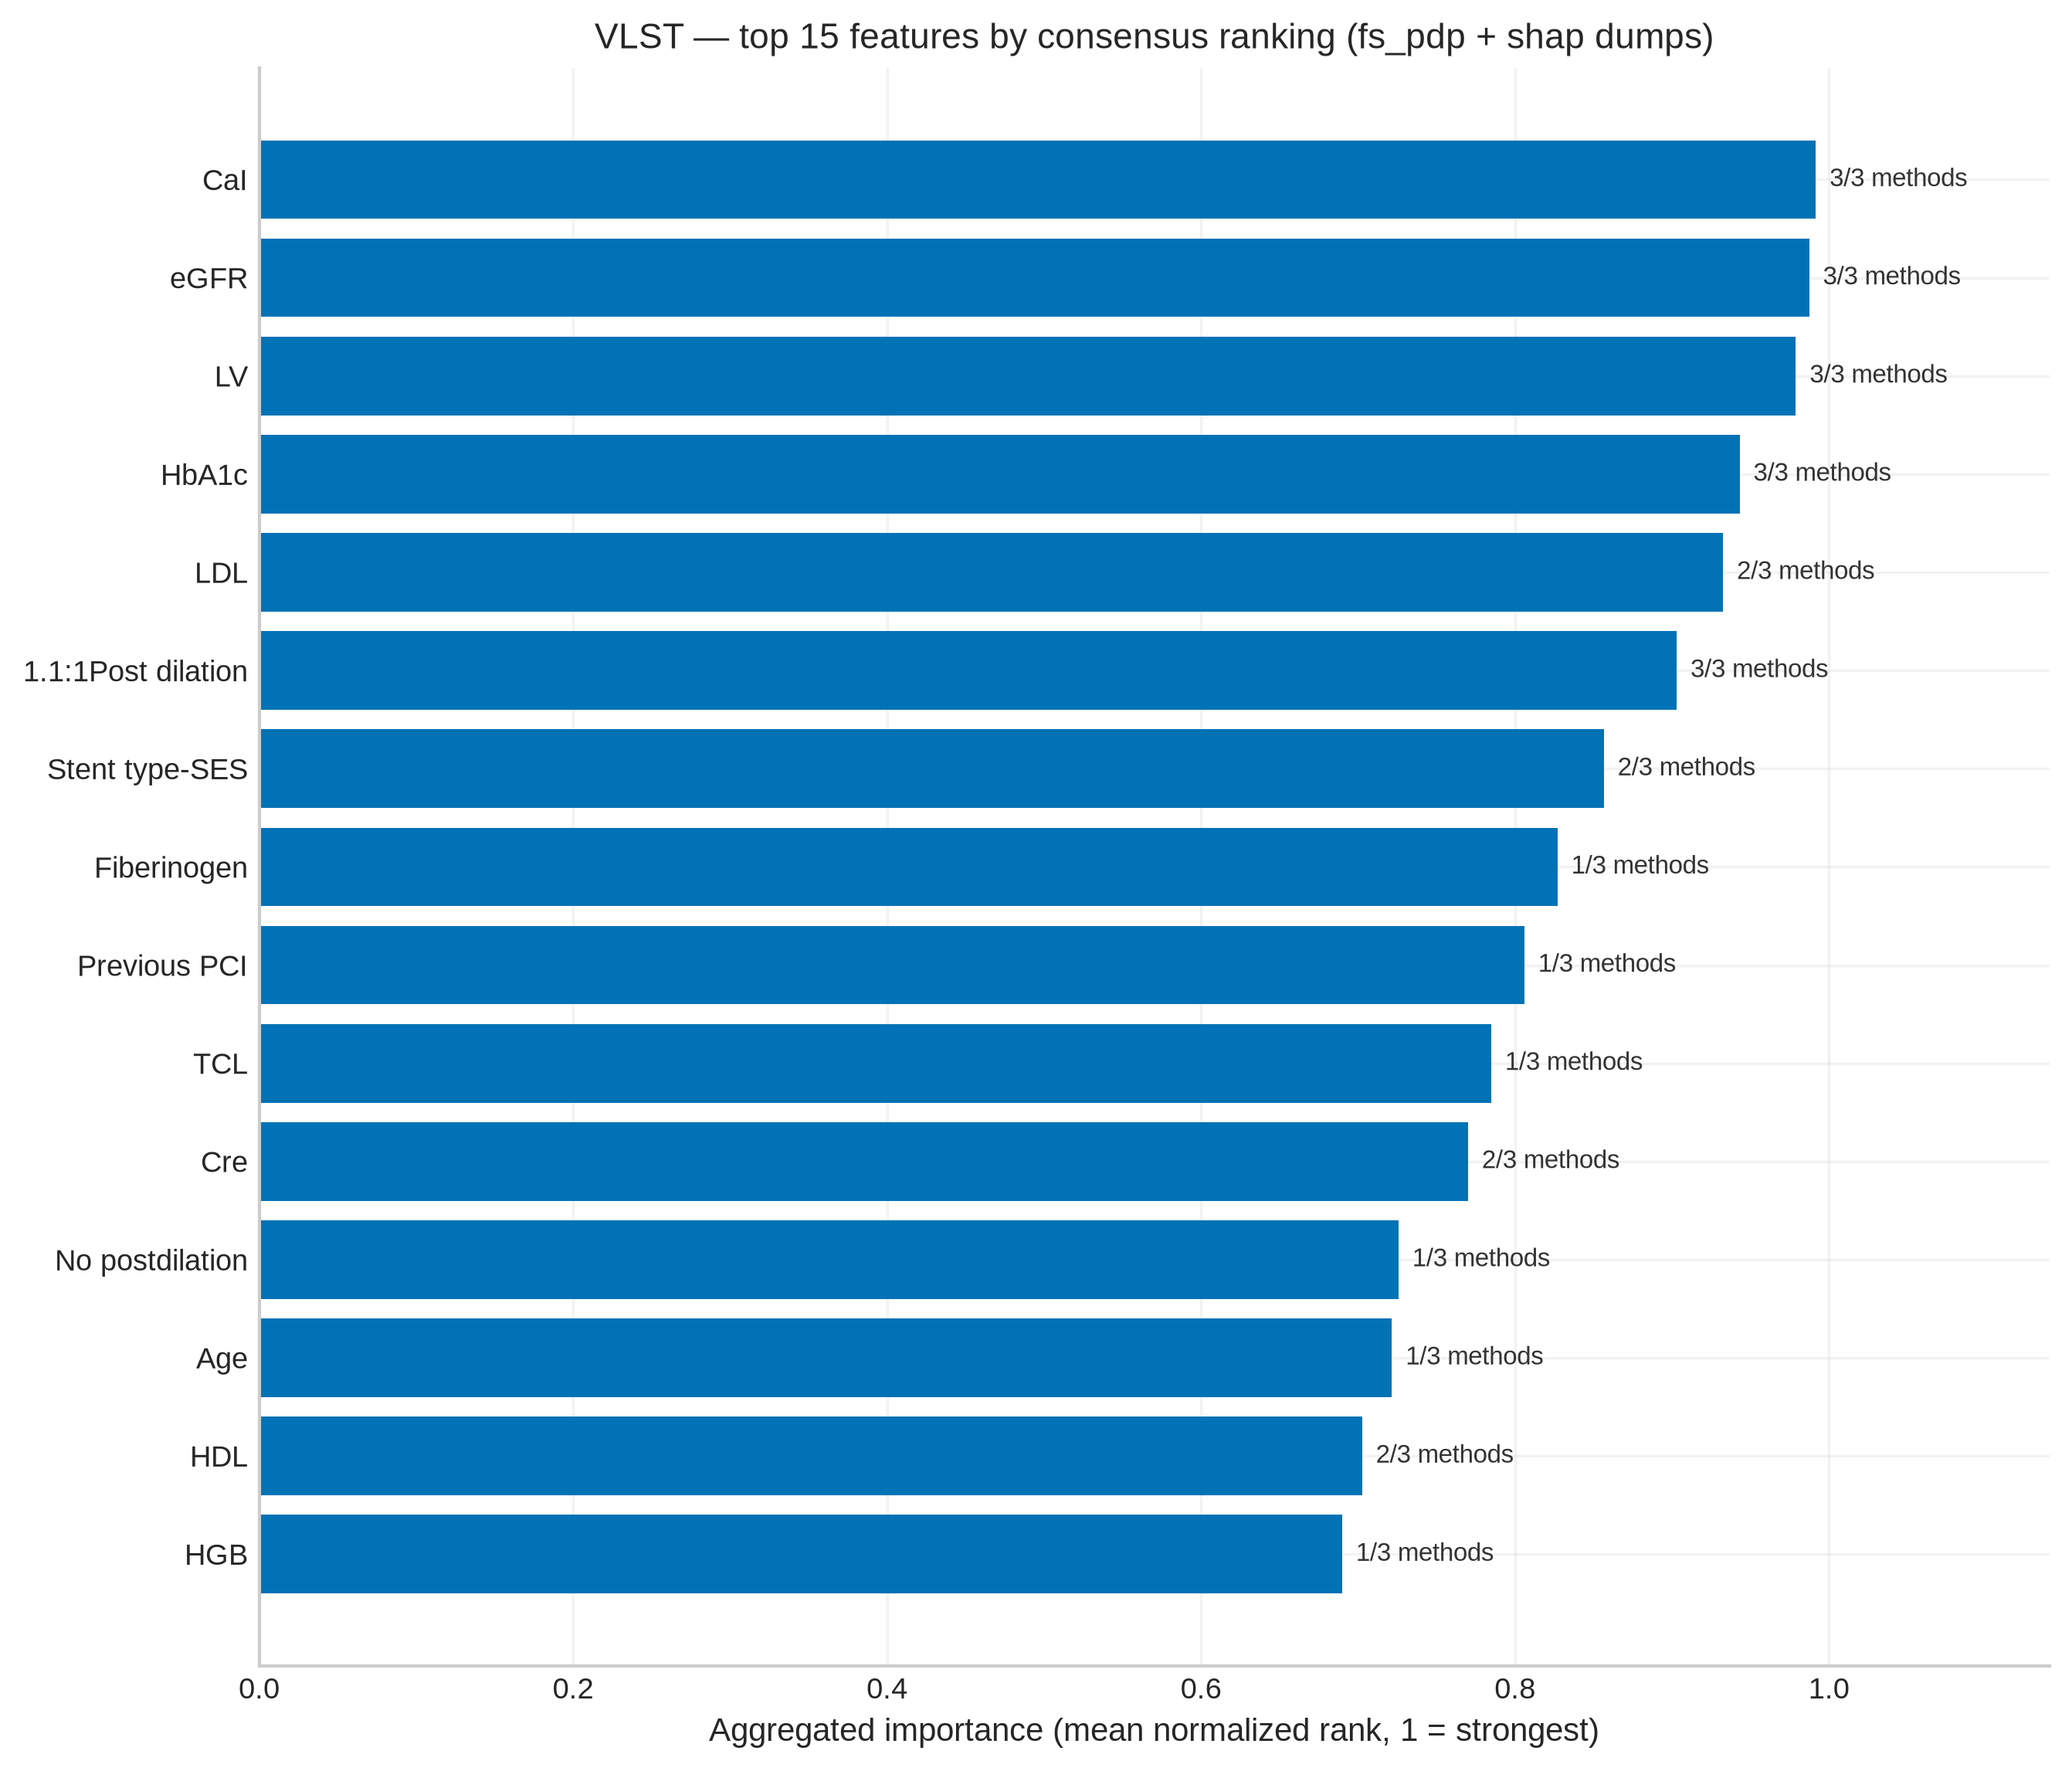
\includegraphics[keepaspectratio,alt={Figure. Consensus ranking}]{../paper_results/05_tabpfn_interpretability/paper_figures/paper_fig13_consensus_ranking.png}}
\caption{Figure. Consensus ranking}
\end{figure}

\begin{center}\rule{0.5\linewidth}{0.5pt}\end{center}

\section{Discussion}\label{discussion}

Numbers are only those frozen in \texttt{paper/frozen\_results.yaml}.
Association ≠ prediction ≠ attribution (\textbf{W5}). No causal, ``risk
factor,'' or clinical-utility claims. Decision-curve analysis is absent
(\textbf{B11}).

\begin{center}\rule{0.5\linewidth}{0.5pt}\end{center}

\subsection{5.1 Principal findings --- TabPFN under extreme imbalance
without a per-dataset
grid}\label{principal-findings-tabpfn-under-extreme-imbalance-without-a-per-dataset-grid}

The ranking result that survives anti-leakage handling is
derivation-cohort nested CV, not a bedside rule. After the full OFF
protocol, TabPFN thinking v3.5 has the highest nested PR-AUC among nine
fitted arms (\textbf{0.9212} {[}0.8785, 0.9613{]}); local TabPFN v3.5 is
second (\textbf{0.8957} {[}0.8446, 0.9426{]}). Both exceed
\textbf{library-default} XGBoost \textbf{0.6322} and LightGBM
\textbf{0.6271} (paired Δ thinking v3.5 − LightGBM \textbf{0.2941}
(0.2071--0.3805), P(Δ ≤ 0) = 0/2000). That is a ranking of these
objects, not ``TabPFN versus tuned boosting.'' Nested F1 at inner-fold
thresholds: thinking v3.5 \textbf{0.8603} (sensitivity 0.8370); local
v3.5 \textbf{0.8229}; LightGBM \textbf{0.5902}.

Why TabPFN can rank above this \textbf{untuned reference panel} on this
file is a design fact, not a mechanistic proof: it is a tabular
foundation model (in-context learning, native categoricals, no
per-dataset grid) on a small-\emph{n} mixed-type table (92 events).
Classics in the nested zoo are library defaults plus class weighting;
the inner loop tunes only the F1 threshold. Unmatched search effort is
part of the \textbf{claim} (W3.8), not only a limitation. v3 and v3.5
are different checkpoints; thinking-high (\texttt{tabpfn-client}, effort
high) and local \texttt{tabpfn} are different objects. Thinking outranks
local within each family on pooled PR-AUC, \textbf{but not in every
fold} (fold 1: local v3.5 0.9365 vs thinking 0.8802). With 18--19 events
per outer fold, fold-to-fold movement is expected. Ranking uses PR-AUC
because prevalence is \textbf{0.0177}; ROC-AUC is high for every arm
(0.865--0.996) and is the less informative scale.

What does \textbf{not} survive is treating a leaks-on 70/30 scoreboard,
or the excluded unlabeled nested dump (thinking \textbf{0.9771} / local
\textbf{0.9635}), as the TabPFN result. \textbf{{[}RE-SOURCE{]}:} there
is no matched 9-arm nested OFF dump, so a numeric ``nested v3.5 ON minus
nested v3.5 OFF'' cannot be written.

\begin{center}\rule{0.5\linewidth}{0.5pt}\end{center}

\subsection{5.2 Clinical context --- stent characteristics and
biomarkers (association /
attribution)}\label{clinical-context-stent-characteristics-and-biomarkers-association-attribution}

Names that recur after anti-leakage, as \textbf{associations or
attributions}, not treatment effects:

\begin{itemize}
\tightlist
\item
  Table 4b (identified logit): post-dilation and Clopidogrel have
  adjusted OR \textless{} 1; WBC, previous PCI, and \texttt{LV} have OR
  \textgreater{} 1. DAPT flags are follow-up persistence after the
  mandated year, not index-PCI prescriptions (W3.6).
\item
  Part 5 stability SFS \textbf{8/8}: \texttt{\{CaI,\ LV,\ eGFR\}}.
  Held-out mean \textbar SHAP\textbar: eGFR 1.2288, CaI 1.0867, Cre
  0.8093, LV 0.4828.
\item
  Part 3 FDR ∩ ML three-way (n = 5): \texttt{Clopidogrel},
  \texttt{HbA1c}, \texttt{LV}, \texttt{No\ postdilation}, \texttt{eGFR}
  (Jaccard 0.20).
\end{itemize}

\texttt{eGFR} and \texttt{LV} appear on both classic-selector and TabPFN
sides. \texttt{CaI} is a TabPFN-train/SHAP name (means match Wang peak
troponin I; still unnamed in the CSV). \texttt{WBC} is FDR-only because
it was dropped from the ML matrix (Wang also excluded WBC from the Cox
score). \emph{k}-SII is one held-out VLST=1 row (cohort 5176). PDP is a
train empirical prior near prevalence. None of this is a locked-in
feature mask for nested CV, a causal stent-technique effect, or a
monitoring rule.

The frozen Wang integer score recovers derivation-cohort ROC-AUC
\textbf{0.8013} (published c = 0.80) with PR-AUC \textbf{0.1032}. Nested
thinking v3.5 PR-AUC 0.9212 versus that integer score is a same-file
comparison of foundation-model OOF against an 8-variable Cox point scale
--- \textbf{not} external validation and not inheritance of Wang's
Shantou test (n = 2,058, c = 0.82, file absent).

\begin{center}\rule{0.5\linewidth}{0.5pt}\end{center}

\subsection{5.3 Methodological insight --- subtle leakage in tabular
cardiovascular
ML}\label{methodological-insight-subtle-leakage-in-tabular-cardiovascular-ml}

The first result that should change how this derivation file is modelled
is not a TabPFN score. A published-style 70/30 GridSearch
\textbf{overstates hold-out ranking} when follow-up time and related
leak flags remain in the matrix (W1). ALL LEAKS ON versus OFF drops
PR-AUC by \textbf{0.30--0.61} (LightGBM 0.9687 → 0.6675; logistic
regression 0.9134 → 0.3431). Random forest F1 falls to \textbf{0}. Those
arms are \textbf{not} ``identical except TSSI'': five flags flip
together, including SMOTE. Nested CV does not import those GridSearch
winners and does not use SMOTE.

\textbf{Incentives, as implemented.} (1) TSSI as a covariate is
binary-ified survival time (time-to-event vs completed follow-up). (2)
WBC is a recording-precision / batch marker (and Wang excluded it from
Cox). (3) Lab quantization is done \textbf{before} splitting so it is
not a \emph{y}-dependent encoder; a signature-only probe (243
indicators, AP 0.4270) shows how far decimal-grid membership alone can
rank. Equalising leftover precision still drops TabPFN v3.5 nested AP by
0.0518. (4) Stent brands are encoded on the \textbf{train fold only} so
rare strings cannot leak from the test distribution. (5) SMOTE is OFF
except the leaks-on twin train set. Companion: identifiers dropped;
scaler/OHE cloned inside splits; Part 2/5 catalogues do not mask nested
CV. Follow-up drugs stay in with a post-baseline caveat. These are
operational choices; they are not a claim that all possible leakage has
been eliminated (brand-frequency leak on the ON arm is not separately
quantified).

\begin{center}\rule{0.5\linewidth}{0.5pt}\end{center}

\subsection{5.4 Limitations}\label{limitations}

\begin{enumerate}
\def\labelenumi{\arabic{enumi}.}
\tightlist
\item
  \textbf{No external or temporal test of the ML models} (W3.1, B11).
  Nested CV on 5,185 derivation rows is not Shantou. Single-centre file
  (The First Hospital of Jilin University).
\item
  \textbf{Binary label versus Wang's Cox time-to-event analysis} (W3.2).
  Dropping TSSI is required for honest binary classification and is not
  a Cox re-fit.
\item
  \textbf{Rare-event statistics / EPV} (W4): 92/81 ≈ \textbf{1.14};
  Table 4 ≈ \textbf{5.4}; Table 4b ≈ \textbf{7.1} (still below EPV ≥
  10); 18--19 events per outer fold.
\item
  \textbf{Retrospective derivation-cohort design}; analysis not
  separately pre-registered.
\item
  Four TabPFN calibrations and two APIs must not be collapsed
  (W3.4--W3.5). Lowest nested ECE is local v3.5 \textbf{0.0003};
  thinking v3.5 ECE \textbf{0.0028}. No decision-curve (B11) --- nested
  PPV at an F1 cut is not clinical utility.
\item
  DAPT columns are post-baseline persistence (W3.6). WBC dual-label
  (W3.7). Unequal tuning (W3.8). Bootstrap does not re-fit (W3.9).
  \texttt{LV} / \texttt{CaI} unnamed (W3.10). Part 5 ≠ Part 4 predictor;
  SHAP dump records HTTP 429 then local finish (W3.11).
\item
  Interpretability was split because a full run exceeds the Kaggle
  session limit. SFS used \textbf{8} seeds, not the abandoned 10-seed
  plan. Client quota (20 thinking fits, 50M cells/day) constrained
  thinking-high design.
\item
  SMOTE only in ALL LEAKS ON. Single nested CV, not repeated. Cox LP /
  Shantou remain absent (B11).
\end{enumerate}

These constraints bound the numbers: association under low EPV,
attribution on a 70/30 split, and nested-CV discrimination on one
derivation file.

\begin{center}\rule{0.5\linewidth}{0.5pt}\end{center}

\subsection{5.5 Conclusion}\label{conclusion}

On Wang 2020's derivation cohort, after the full ALL LEAKS OFF protocol,
TabPFN thinking v3.5 had the highest nested-CV PR-AUC among nine fitted
arms (0.9212); local TabPFN v3.5 (0.8957) also exceeded library-default
XGBoost (0.6322) and LightGBM (0.6271). That is not a
hyperparameter-matched contest against tuned boosting. TSSI, WBC, raw
lab decimals, a full-cohort stent codebook, and train SMOTE must not
enter nested-CV binary classifiers as if they were baseline covariates.
Recurring names in association and attribution (\texttt{eGFR},
\texttt{LV}, post-dilation flags, \texttt{CaI} on the TabPFN side) are
not treatment effects. Nested-CV discrimination on this file is not
external validation; the ML models were not externally or temporally
tested.

\begin{center}\rule{0.5\linewidth}{0.5pt}\end{center}

\section{Tables and figures}\label{tables-and-figures}

Markdown tables and figures only. Raw LaTeX is not used here (it does
not render in the Markdown paper). Numbers from
\texttt{paper/frozen\_results.yaml}. Optimistic pooled F1 is
\textbf{excluded}. Evidence-map §7.1 historical 0.8553 is \textbf{not}
used.

Paths are relative to \texttt{manuscript/} so they display in
\texttt{main\_paper.md}.

\begin{center}\rule{0.5\linewidth}{0.5pt}\end{center}

\subsection{Table 1. Cohort characteristics (association, not
prediction)}\label{table-1.-cohort-characteristics-association-not-prediction}

Wang 2020 derivation file; n = 5,185 (no VLST 5,093; VLST 92).
Continuous cells: mean (SD). Binary cells: n (\%). Tests as in
\texttt{eda.ipynb}. TSSI omitted (time-at-risk). DAPT is follow-up
persistence. \texttt{LV} and \texttt{CaI} unnamed.

\begin{figure}
\centering
\pandocbounded{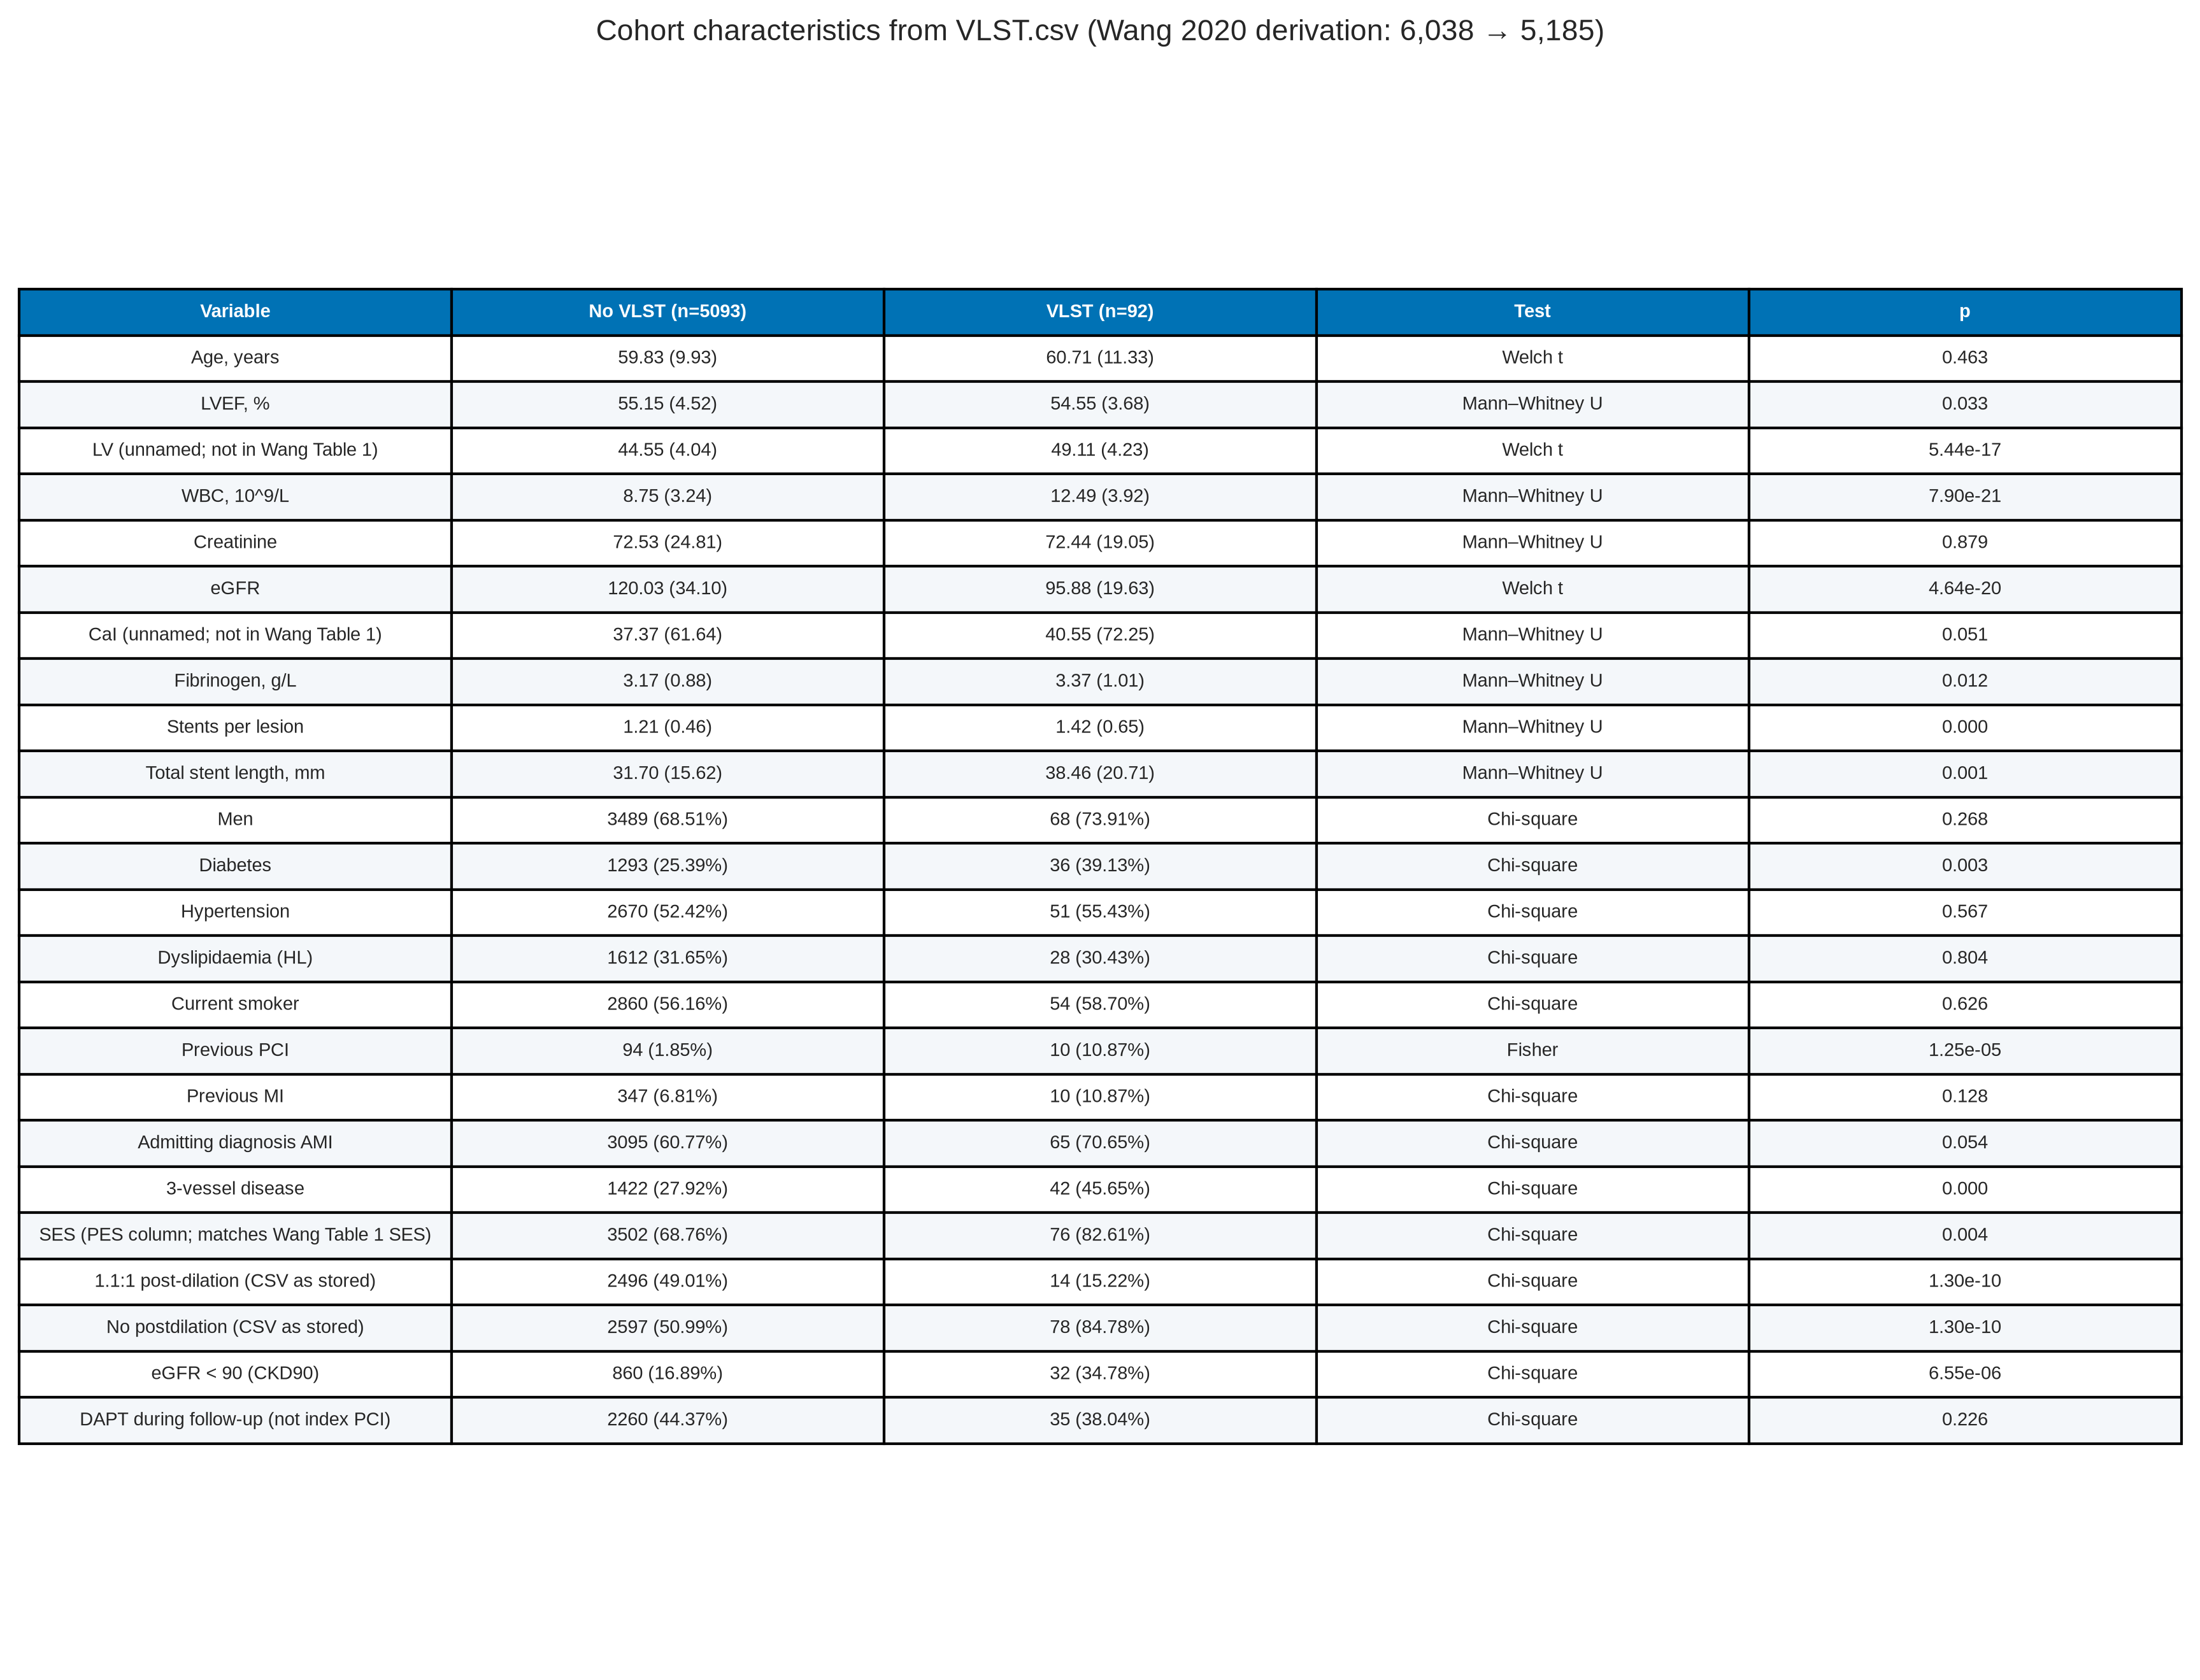
\includegraphics[keepaspectratio,alt={Table 1. Cohort characteristics}]{../paper_results/01_eda/paper_figures/paper_table_c_cohort_characteristics.png}}
\caption{Table 1. Cohort characteristics}
\end{figure}

\textbf{Table 1.} Restyle of
\texttt{paper\_table\_c\_cohort\_characteristics.png}. Numeric copy:

{\def\LTcaptype{none} % do not increment counter
\begin{longtable}[]{@{}
  >{\raggedright\arraybackslash}p{(\linewidth - 8\tabcolsep) * \real{0.1875}}
  >{\raggedright\arraybackslash}p{(\linewidth - 8\tabcolsep) * \real{0.1875}}
  >{\raggedright\arraybackslash}p{(\linewidth - 8\tabcolsep) * \real{0.1875}}
  >{\raggedright\arraybackslash}p{(\linewidth - 8\tabcolsep) * \real{0.1875}}
  >{\raggedleft\arraybackslash}p{(\linewidth - 8\tabcolsep) * \real{0.2500}}@{}}
\toprule\noalign{}
\begin{minipage}[b]{\linewidth}\raggedright
Characteristic
\end{minipage} & \begin{minipage}[b]{\linewidth}\raggedright
No VLST (n = 5,093)
\end{minipage} & \begin{minipage}[b]{\linewidth}\raggedright
VLST (n = 92)
\end{minipage} & \begin{minipage}[b]{\linewidth}\raggedright
Test
\end{minipage} & \begin{minipage}[b]{\linewidth}\raggedleft
\emph{p}
\end{minipage} \\
\midrule\noalign{}
\endhead
\bottomrule\noalign{}
\endlastfoot
Age, years & 59.83 (9.93) & 60.71 (11.33) & Welch & 0.463 \\
Men & 3489 (68.51\%) & 68 (73.91\%) & χ² & 0.268 \\
Diabetes & 1293 (25.39\%) & 36 (39.13\%) & χ² & 0.003 \\
Hypertension & 2670 (52.42\%) & 51 (55.43\%) & χ² & 0.567 \\
Previous PCI & 94 (1.85\%) & 10 (10.87\%) & Fisher & 1.25e-05 \\
Previous MI & 347 (6.81\%) & 10 (10.87\%) & χ² & 0.128 \\
Admitting diagnosis AMI & 3095 (60.77\%) & 65 (70.65\%) & χ² & 0.054 \\
3-vessel disease & 1422 (27.92\%) & 42 (45.65\%) & χ² & 0.000 \\
LVEF, \% & 55.15 (4.52) & 54.55 (3.68) & MW & 0.033 \\
LV (unnamed) & 44.55 (4.04) & 49.11 (4.23) & Welch & 5.44e-17 \\
WBC, 10⁹/L & 8.75 (3.24) & 12.49 (3.92) & MW & 7.90e-21 \\
Creatinine & 72.53 (24.81) & 72.44 (19.05) & MW & 0.879 \\
eGFR & 120.03 (34.10) & 95.88 (19.63) & Welch & 4.64e-20 \\
CaI (unnamed) & 37.37 (61.64) & 40.55 (72.25) & MW & 0.051 \\
Fibrinogen (\texttt{Fiberinogen}) & 3.17 (0.88) & 3.37 (1.01) & MW &
0.012 \\
Stents per lesion & 1.21 (0.46) & 1.42 (0.65) & MW & 0.000 \\
Total stent length, mm & 31.70 (15.62) & 38.46 (20.71) & MW & 0.001 \\
SES (\texttt{PES} column) & 3502 (68.76\%) & 76 (82.61\%) & χ² &
0.004 \\
1.1:1 post-dilation (as stored) & 2496 (49.01\%) & 14 (15.22\%) & χ² &
1.30e-10 \\
No postdilation (complement) & 2597 (50.99\%) & 78 (84.78\%) & χ² &
1.30e-10 \\
eGFR \textless{} 90 (\texttt{CKD90}) & 860 (16.89\%) & 32 (34.78\%) & χ²
& 6.55e-06 \\
DAPT during follow-up & 2260 (44.37\%) & 35 (38.04\%) & χ² & 0.226 \\
\end{longtable}
}

\begin{center}\rule{0.5\linewidth}{0.5pt}\end{center}

\subsection{Table 2. Leakage contrast (ALL LEAKS ON vs ALL LEAKS
OFF)}\label{table-2.-leakage-contrast-all-leaks-on-vs-all-leaks-off}

Stratified 70/30 hold-out (1,556 rows / 28 events). Seven classics,
GridSearchCV. \textbf{Not nested CV. Not TabPFN.} Δ = ON − OFF. Gaussian
NB ROC dual-labelled (higher OFF). RF F1 OFF = 0.

\begin{figure}
\centering
\pandocbounded{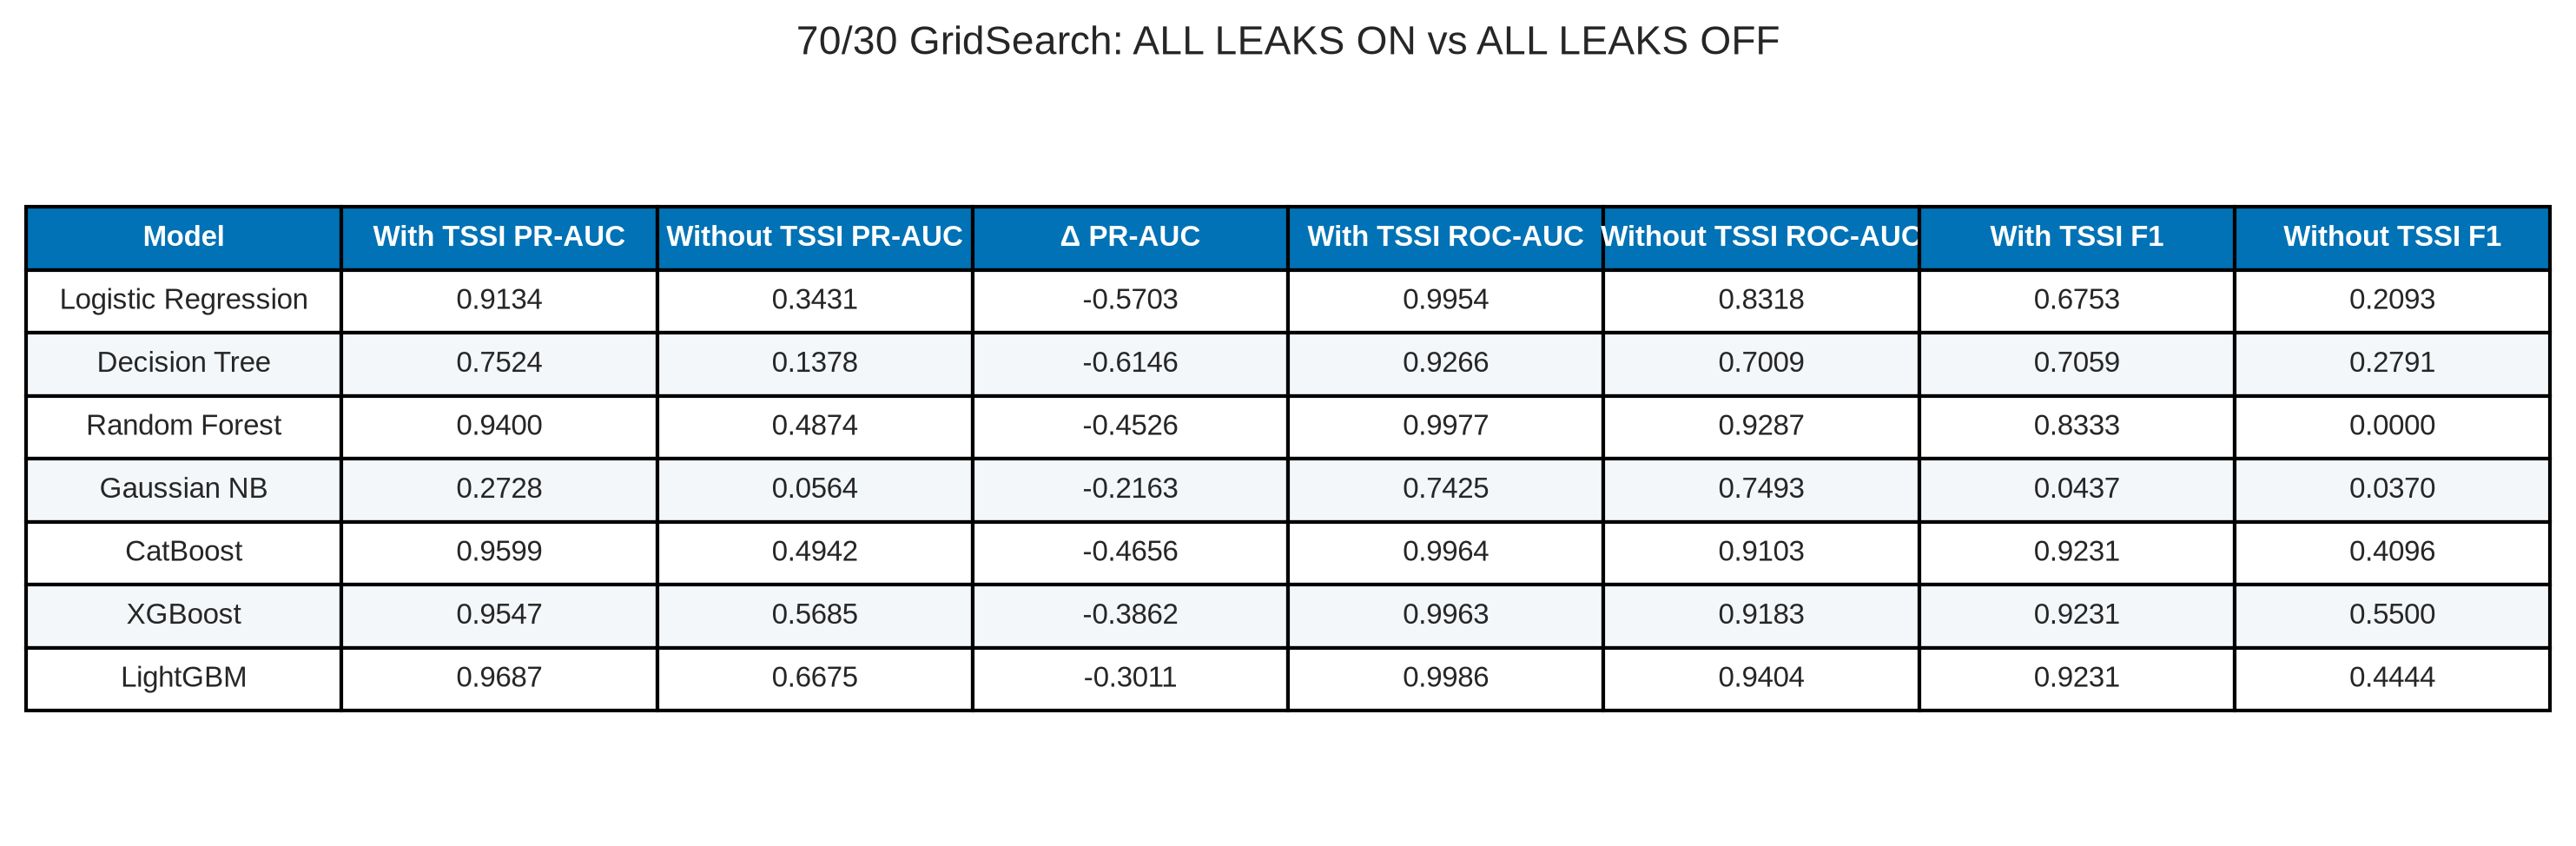
\includegraphics[keepaspectratio,alt={Table 2. Leakage metrics}]{../paper_results/04_tabpfn_rating/paper_figures/paper_table_s_tssi_leakage.png}}
\caption{Table 2. Leakage metrics}
\end{figure}

\textbf{Figure S-TSSI.} PR-AUC collapse on the 1,556-row hold-out.
Dotted line = prevalence 0.0177.

\begin{figure}
\centering
\pandocbounded{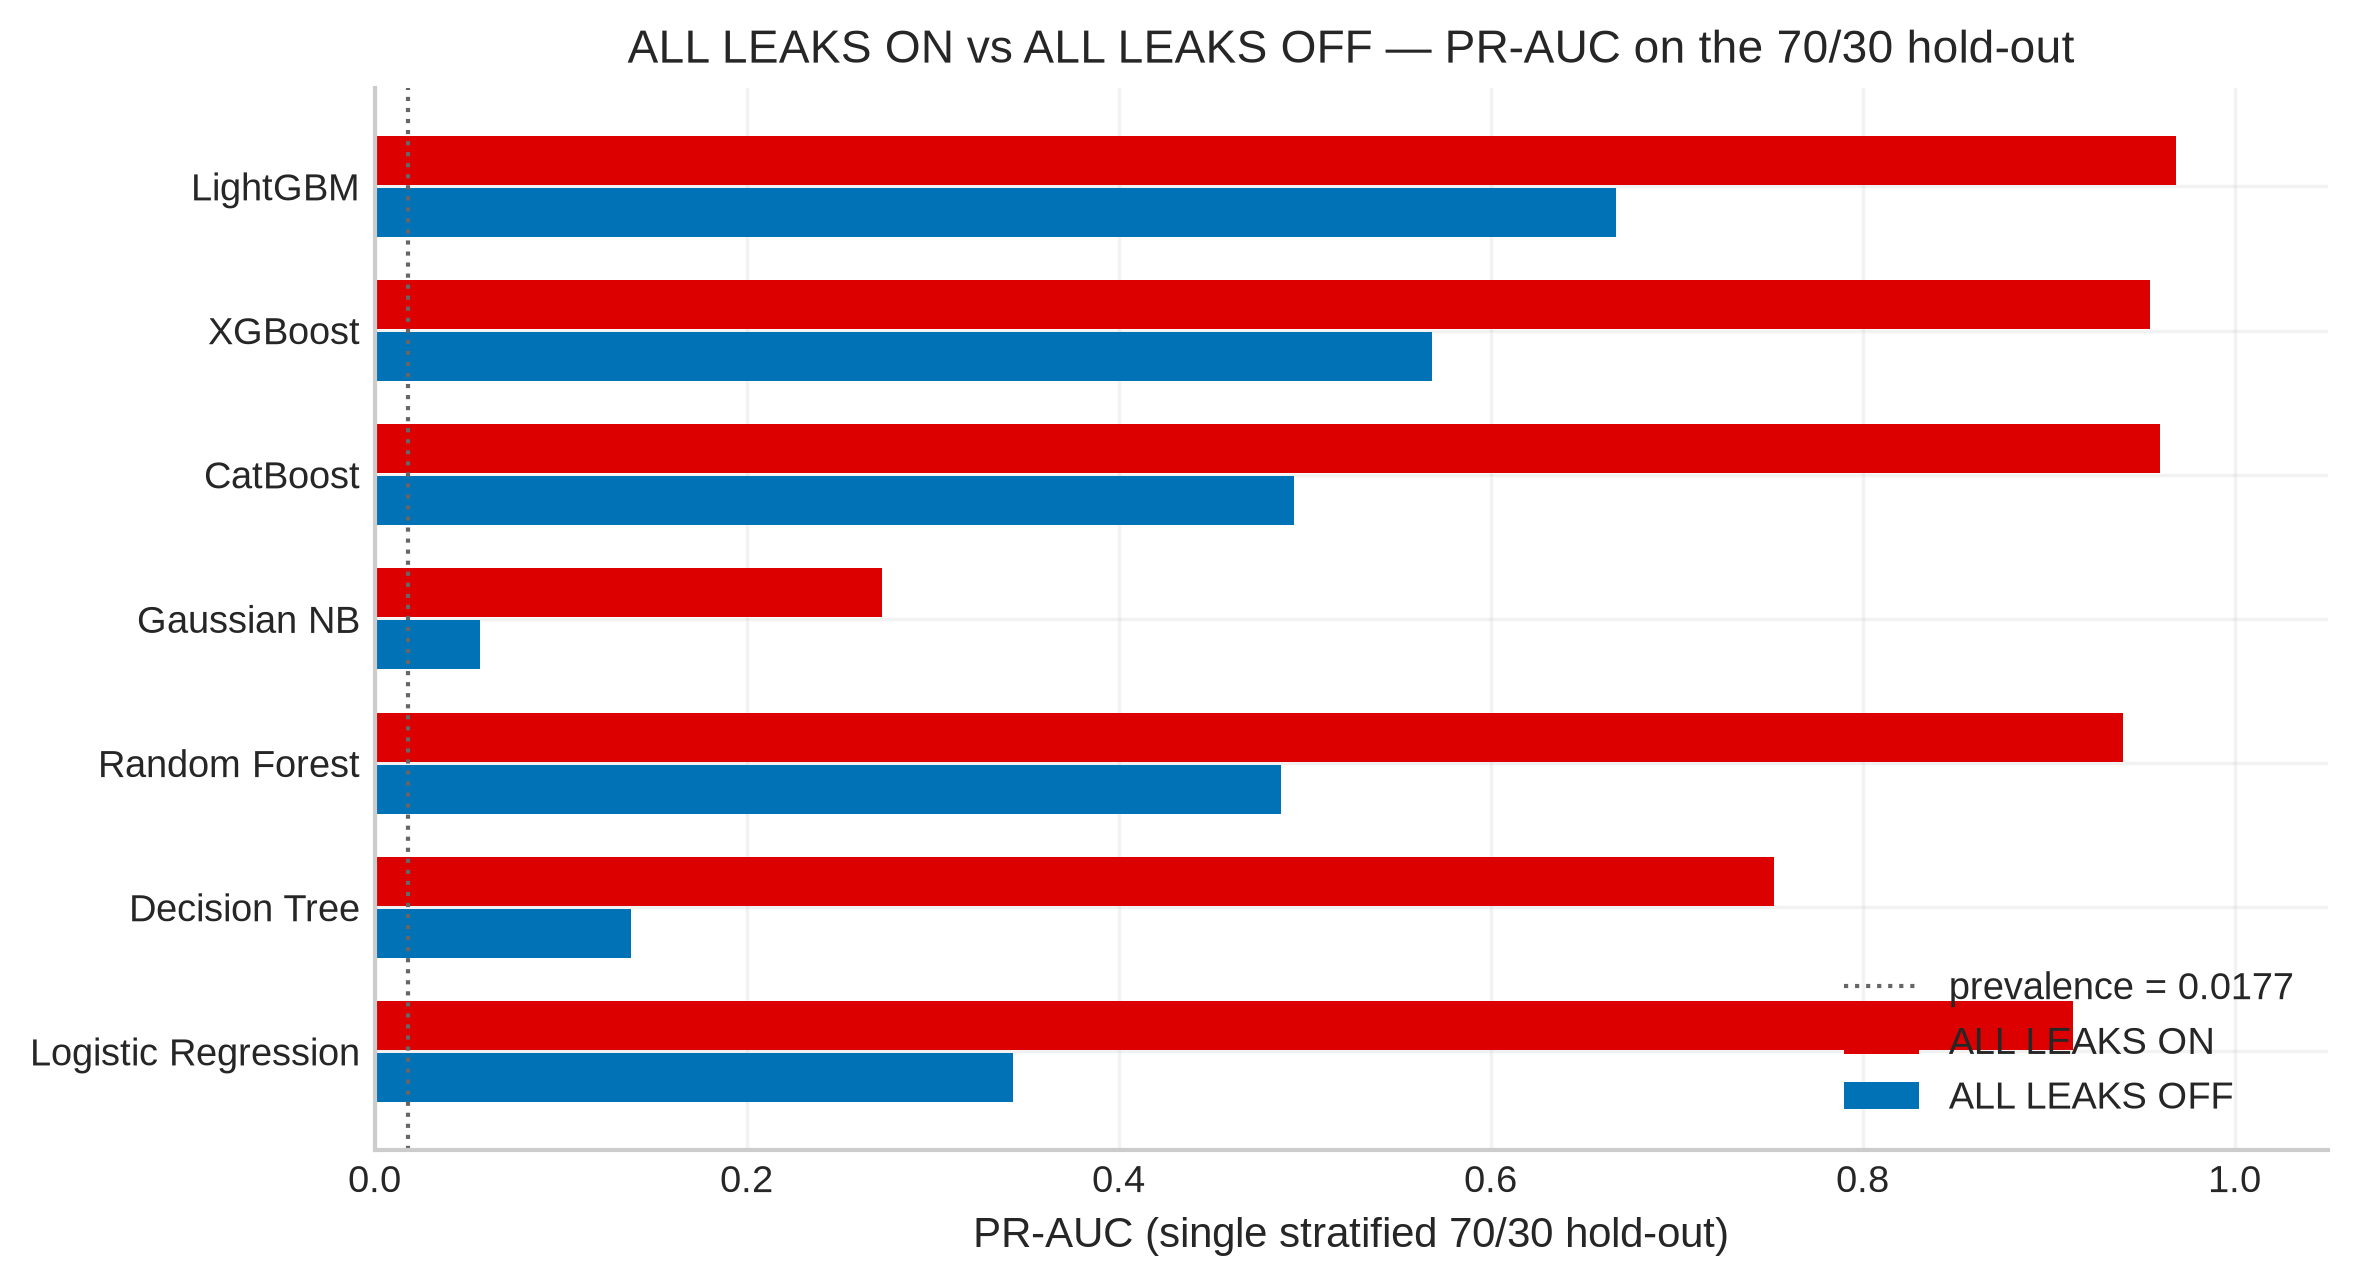
\includegraphics[keepaspectratio,alt={Figure S-TSSI. PR-AUC ON vs OFF}]{../paper_results/04_tabpfn_rating/paper_figures/paper_fig_s_tssi_pr_auc.png}}
\caption{Figure S-TSSI. PR-AUC ON vs OFF}
\end{figure}

\textbf{2a. PR-AUC}

{\def\LTcaptype{none} % do not increment counter
\begin{longtable}[]{@{}lrrr@{}}
\toprule\noalign{}
Model & ON & OFF & Δ \\
\midrule\noalign{}
\endhead
\bottomrule\noalign{}
\endlastfoot
Logistic regression & 0.9134 & 0.3431 & +0.5703 \\
Decision tree & 0.7524 & 0.1378 & +0.6146 \\
Random forest & 0.9400 & 0.4874 & +0.4526 \\
Gaussian NB & 0.2728 & 0.0564 & +0.2163 \\
CatBoost & 0.9599 & 0.4942 & +0.4656 \\
XGBoost & 0.9547 & 0.5685 & +0.3862 \\
LightGBM & 0.9687 & 0.6675 & +0.3011 \\
\end{longtable}
}

\textbf{2b. F1 at the notebook cut}

{\def\LTcaptype{none} % do not increment counter
\begin{longtable}[]{@{}lrr@{}}
\toprule\noalign{}
Model & F1 ON & F1 OFF \\
\midrule\noalign{}
\endhead
\bottomrule\noalign{}
\endlastfoot
Logistic regression & 0.6753 & 0.2093 \\
Decision tree & 0.7059 & 0.2791 \\
Random forest & 0.8333 & \textbf{0.0000} \\
Gaussian NB & 0.0437 & 0.0370 \\
CatBoost & 0.9231 & 0.4096 \\
XGBoost & 0.9231 & 0.5500 \\
LightGBM & 0.9231 & 0.4444 \\
\end{longtable}
}

Dump ROC/PR curves:

\begin{figure}
\centering
\pandocbounded{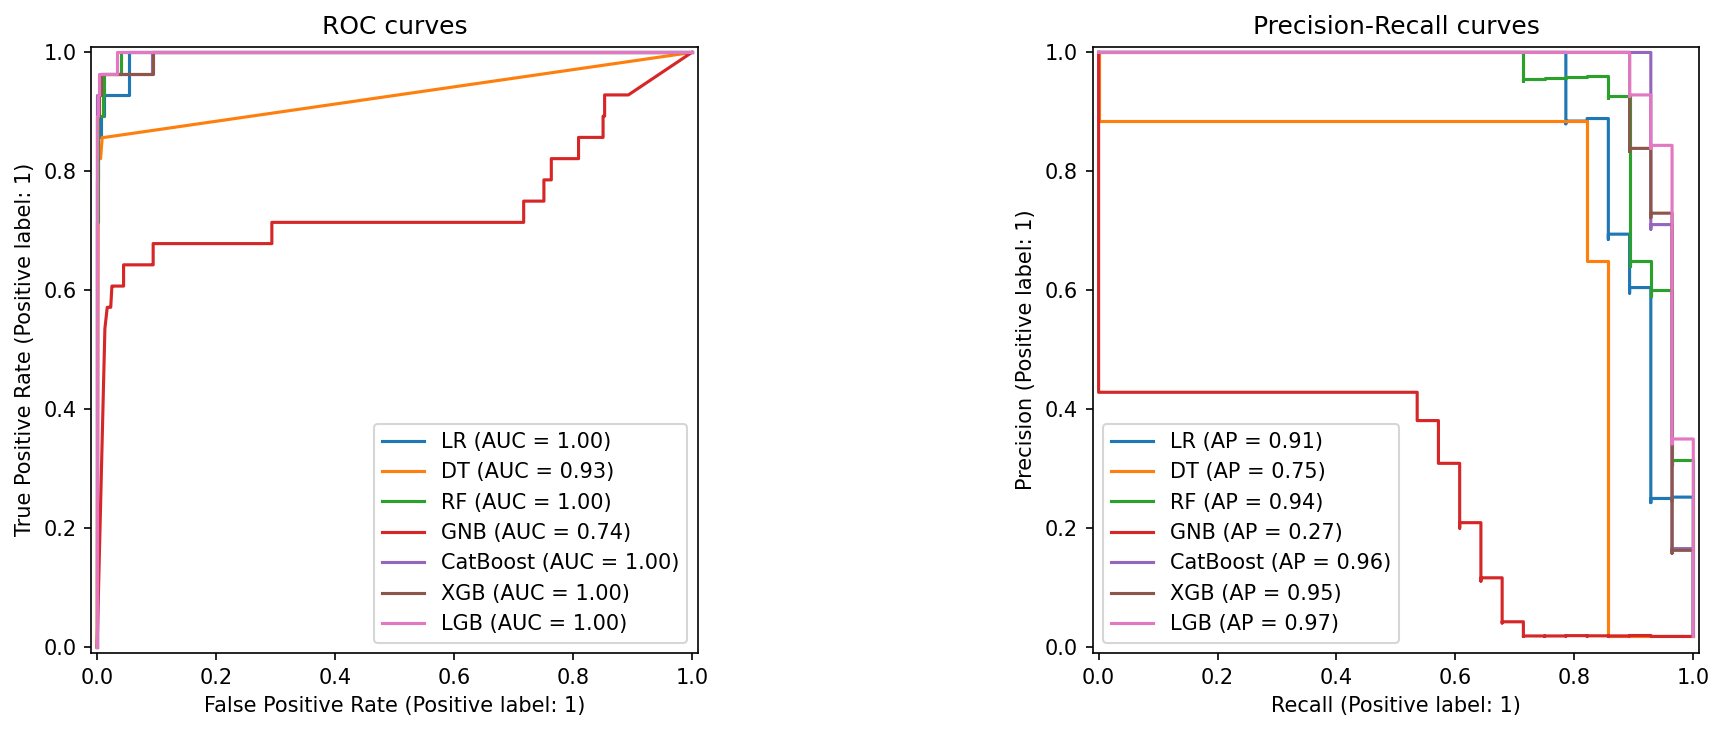
\includegraphics[keepaspectratio,alt={ALL LEAKS ON ROC/PR}]{../paper_results/04_tabpfn_rating/paper_figures/paper_fig_s_leakage_roc_pr_on.png}}
\caption{ALL LEAKS ON ROC/PR}
\end{figure}

\begin{figure}
\centering
\pandocbounded{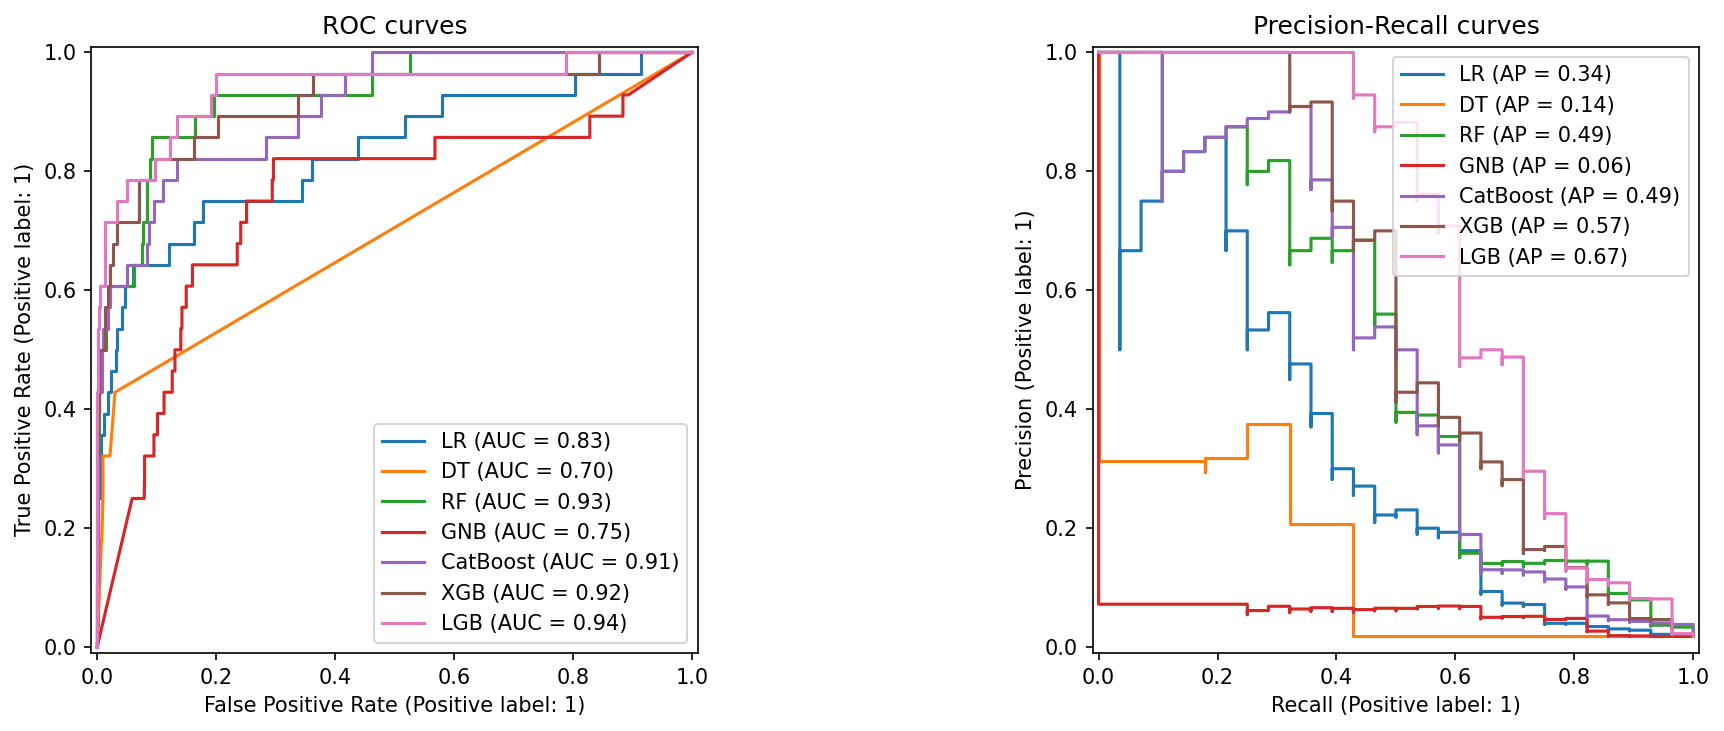
\includegraphics[keepaspectratio,alt={ALL LEAKS OFF ROC/PR}]{../paper_results/04_tabpfn_rating/paper_figures/paper_fig_s_leakage_roc_pr_off.png}}
\caption{ALL LEAKS OFF ROC/PR}
\end{figure}

\begin{center}\rule{0.5\linewidth}{0.5pt}\end{center}

\subsection{Table 3. Nested-CV benchmark (anti-leakage ON, 9
arms)}\label{table-3.-nested-cv-benchmark-anti-leakage-on-9-arms}

Pooled OOF ranking + honest nested operating point (inner-fold F1
thresholds). Anti-leakage ON = ALL LEAKS OFF. Five classic rows are
\textbf{library defaults + class weights}, not nested GridSearch.
Bootstrap 95\% CIs on PR-AUC (\texttt{n\_boot=2000}, seed 42). Pins
\texttt{tabpfn==9.0.0} / \texttt{tabpfn-client==0.6.0}. Do \textbf{not}
quote pooled F1 cuts instead of nested Table 2.

\textbf{Figure 1.} Nested-CV out-of-fold PR (left) and ROC (right).

\begin{figure}
\centering
\pandocbounded{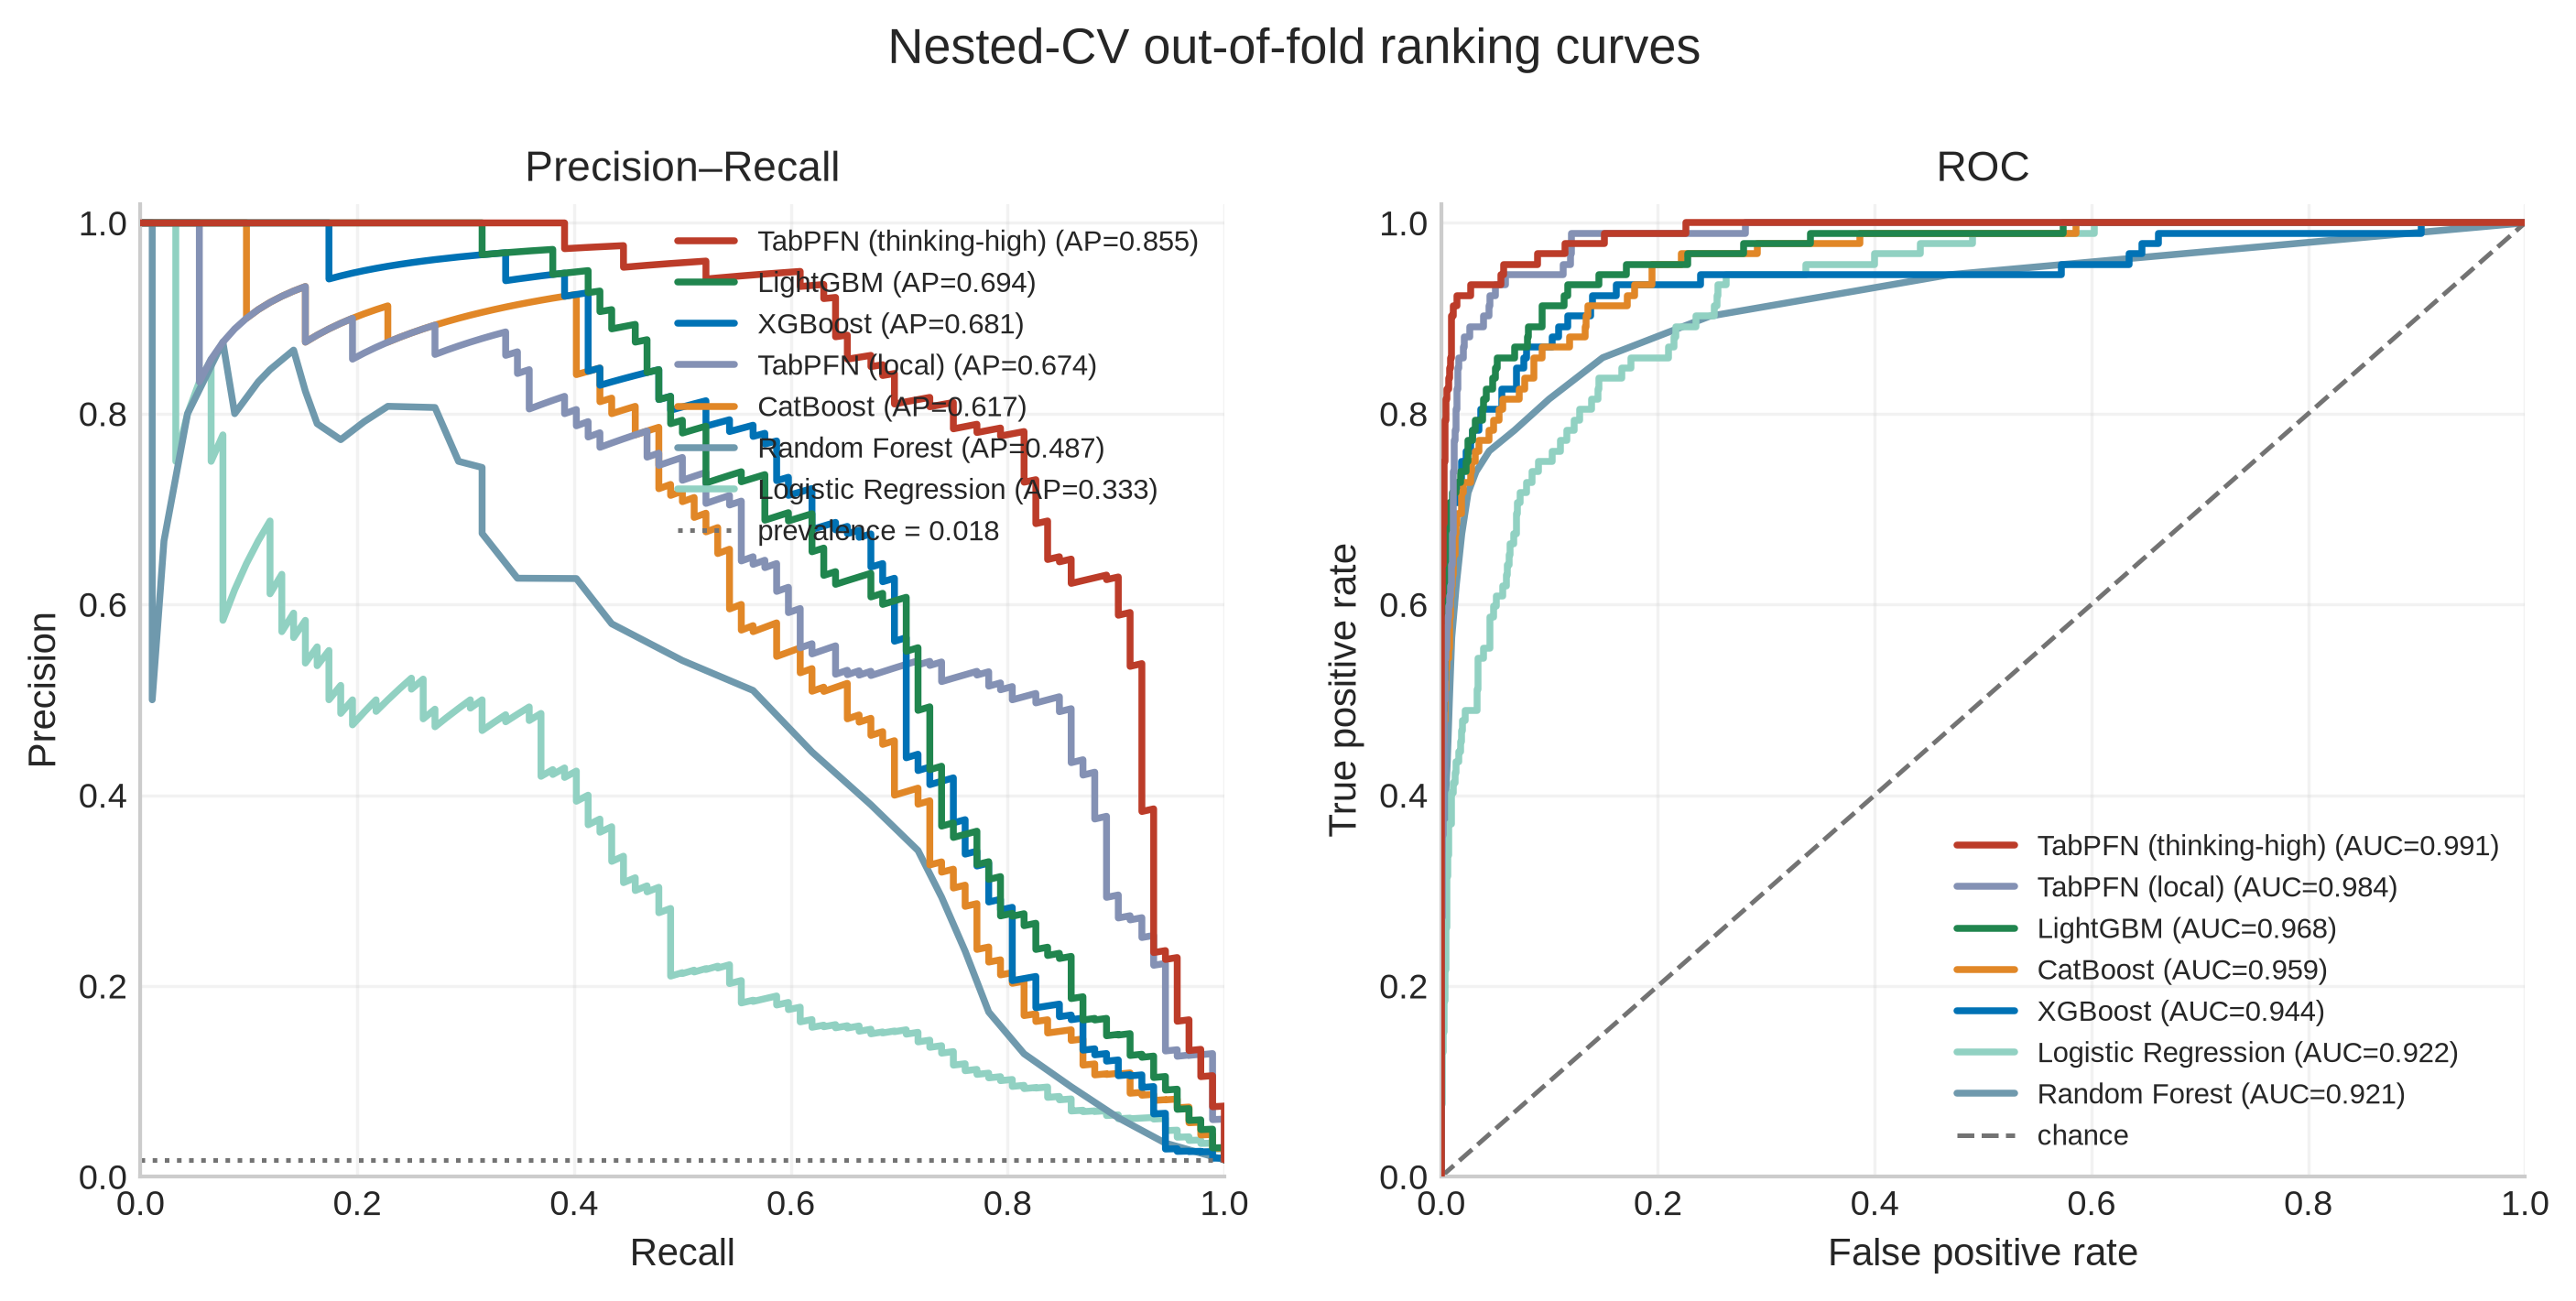
\includegraphics[keepaspectratio,alt={Figure 1. Nested OOF PR and ROC}]{../paper_results/04_tabpfn_rating/paper_figures/paper_fig1_pr_roc_curves.png}}
\caption{Figure 1. Nested OOF PR and ROC}
\end{figure}

\textbf{Figure 2.} Nested-CV calibration (quantile bins).

\begin{figure}
\centering
\pandocbounded{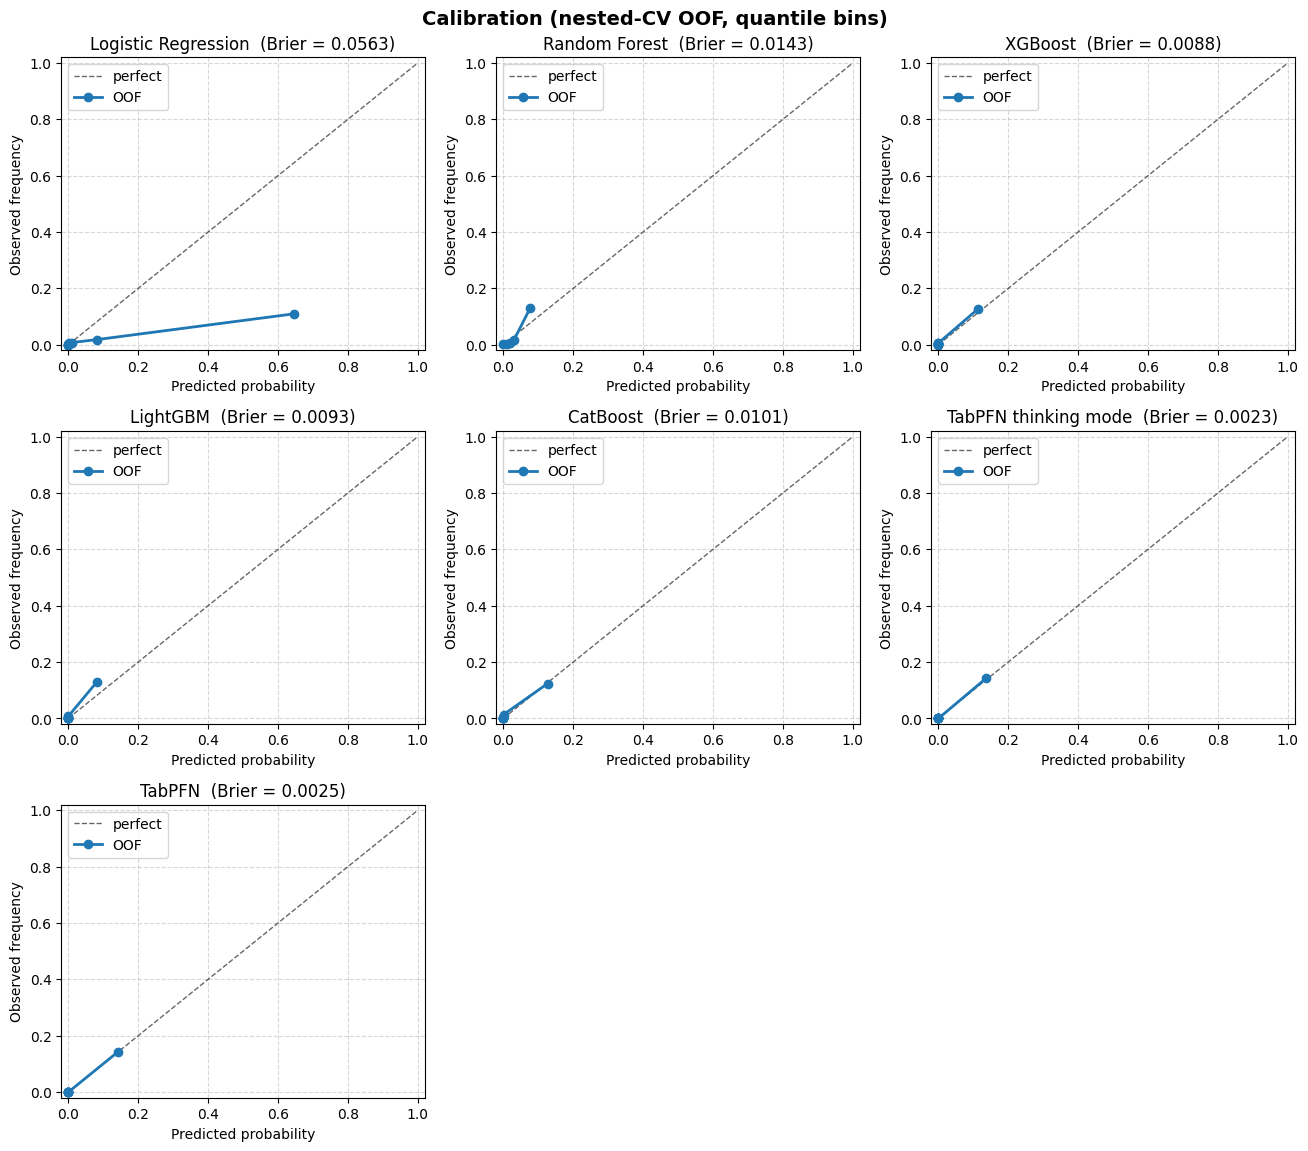
\includegraphics[keepaspectratio,alt={Figure 2. Nested calibration}]{../paper_results/04_tabpfn_rating/paper_figures/paper_fig2_calibration_curves.png}}
\caption{Figure 2. Nested calibration}
\end{figure}

\begin{figure}
\centering
\pandocbounded{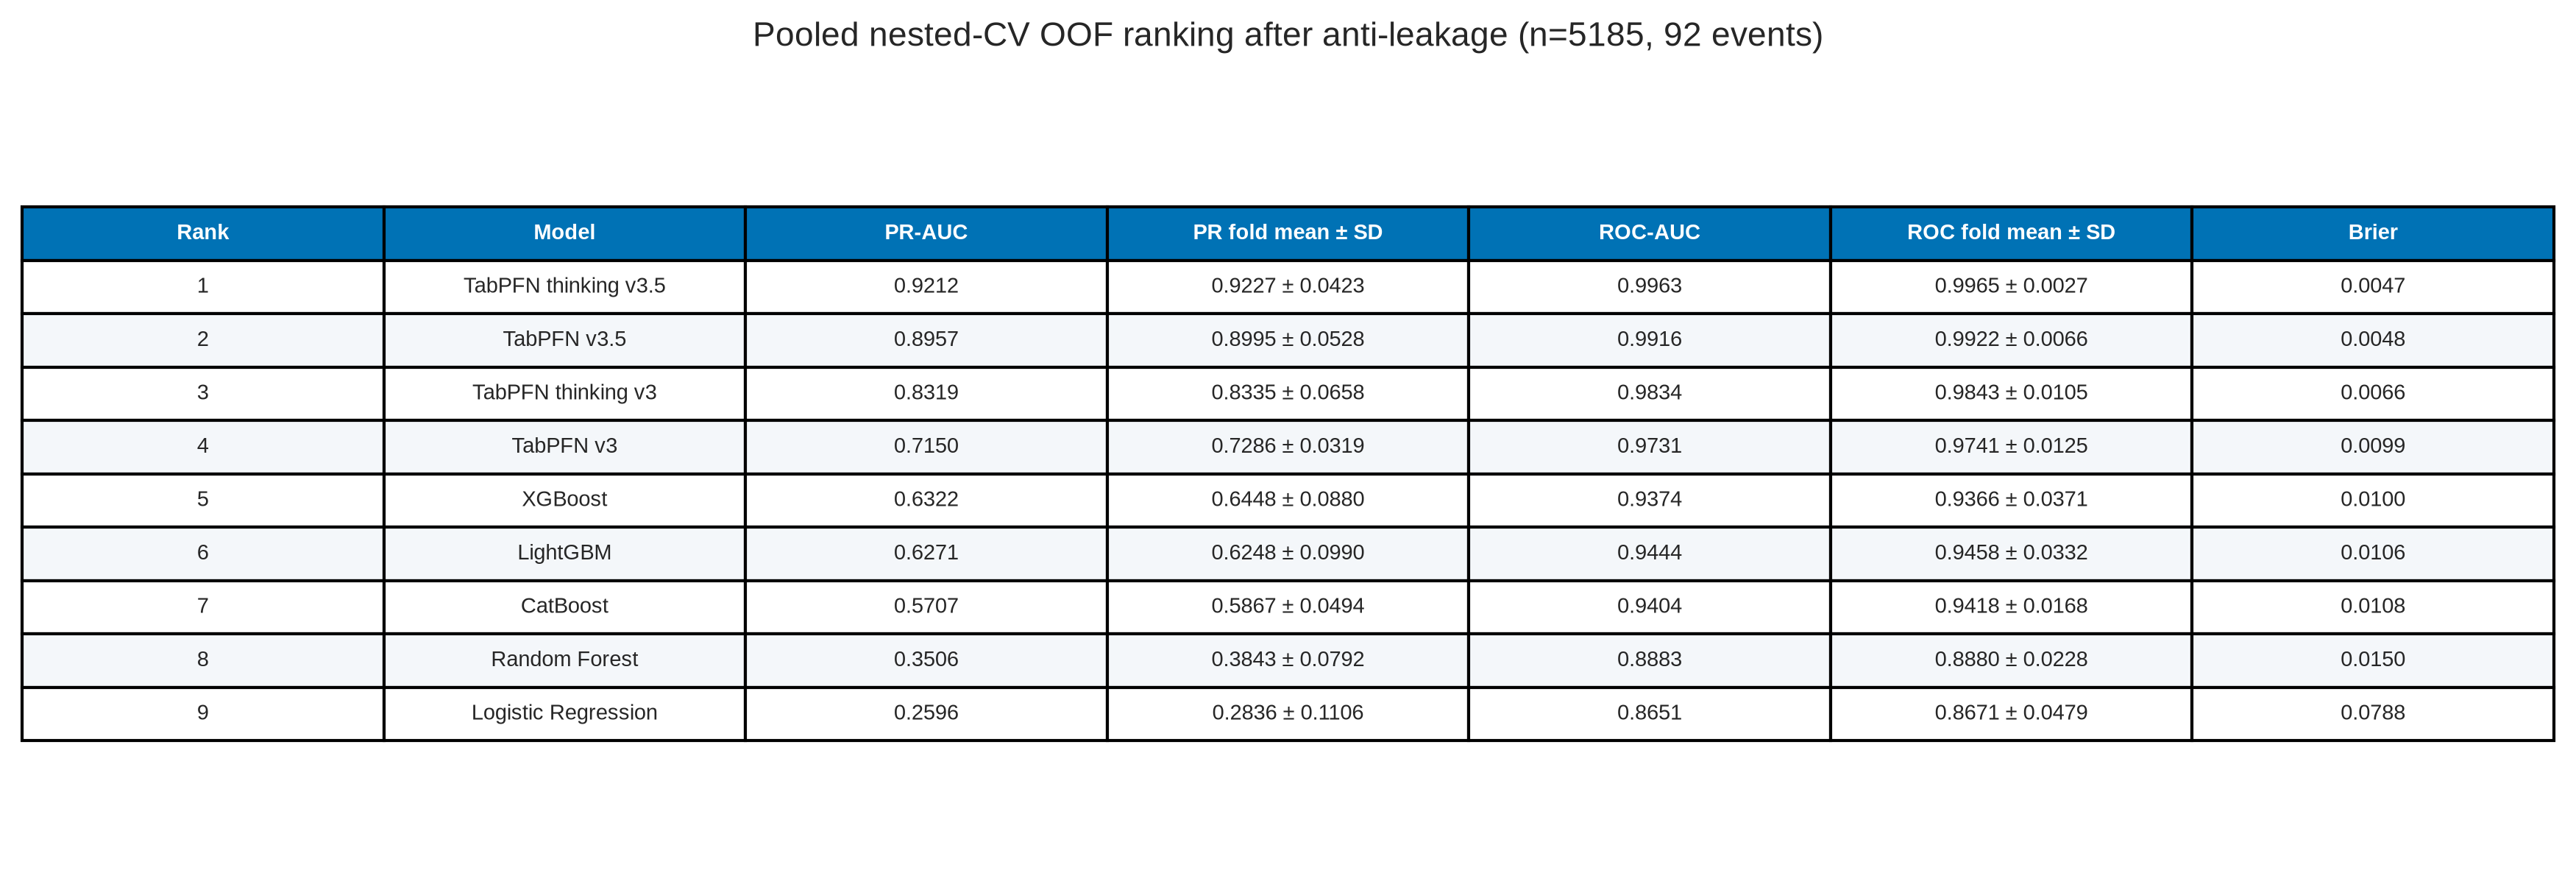
\includegraphics[keepaspectratio,alt={Ranking metrics table}]{../paper_results/04_tabpfn_rating/paper_figures/paper_table1_ranking.png}}
\caption{Ranking metrics table}
\end{figure}

\begin{figure}
\centering
\pandocbounded{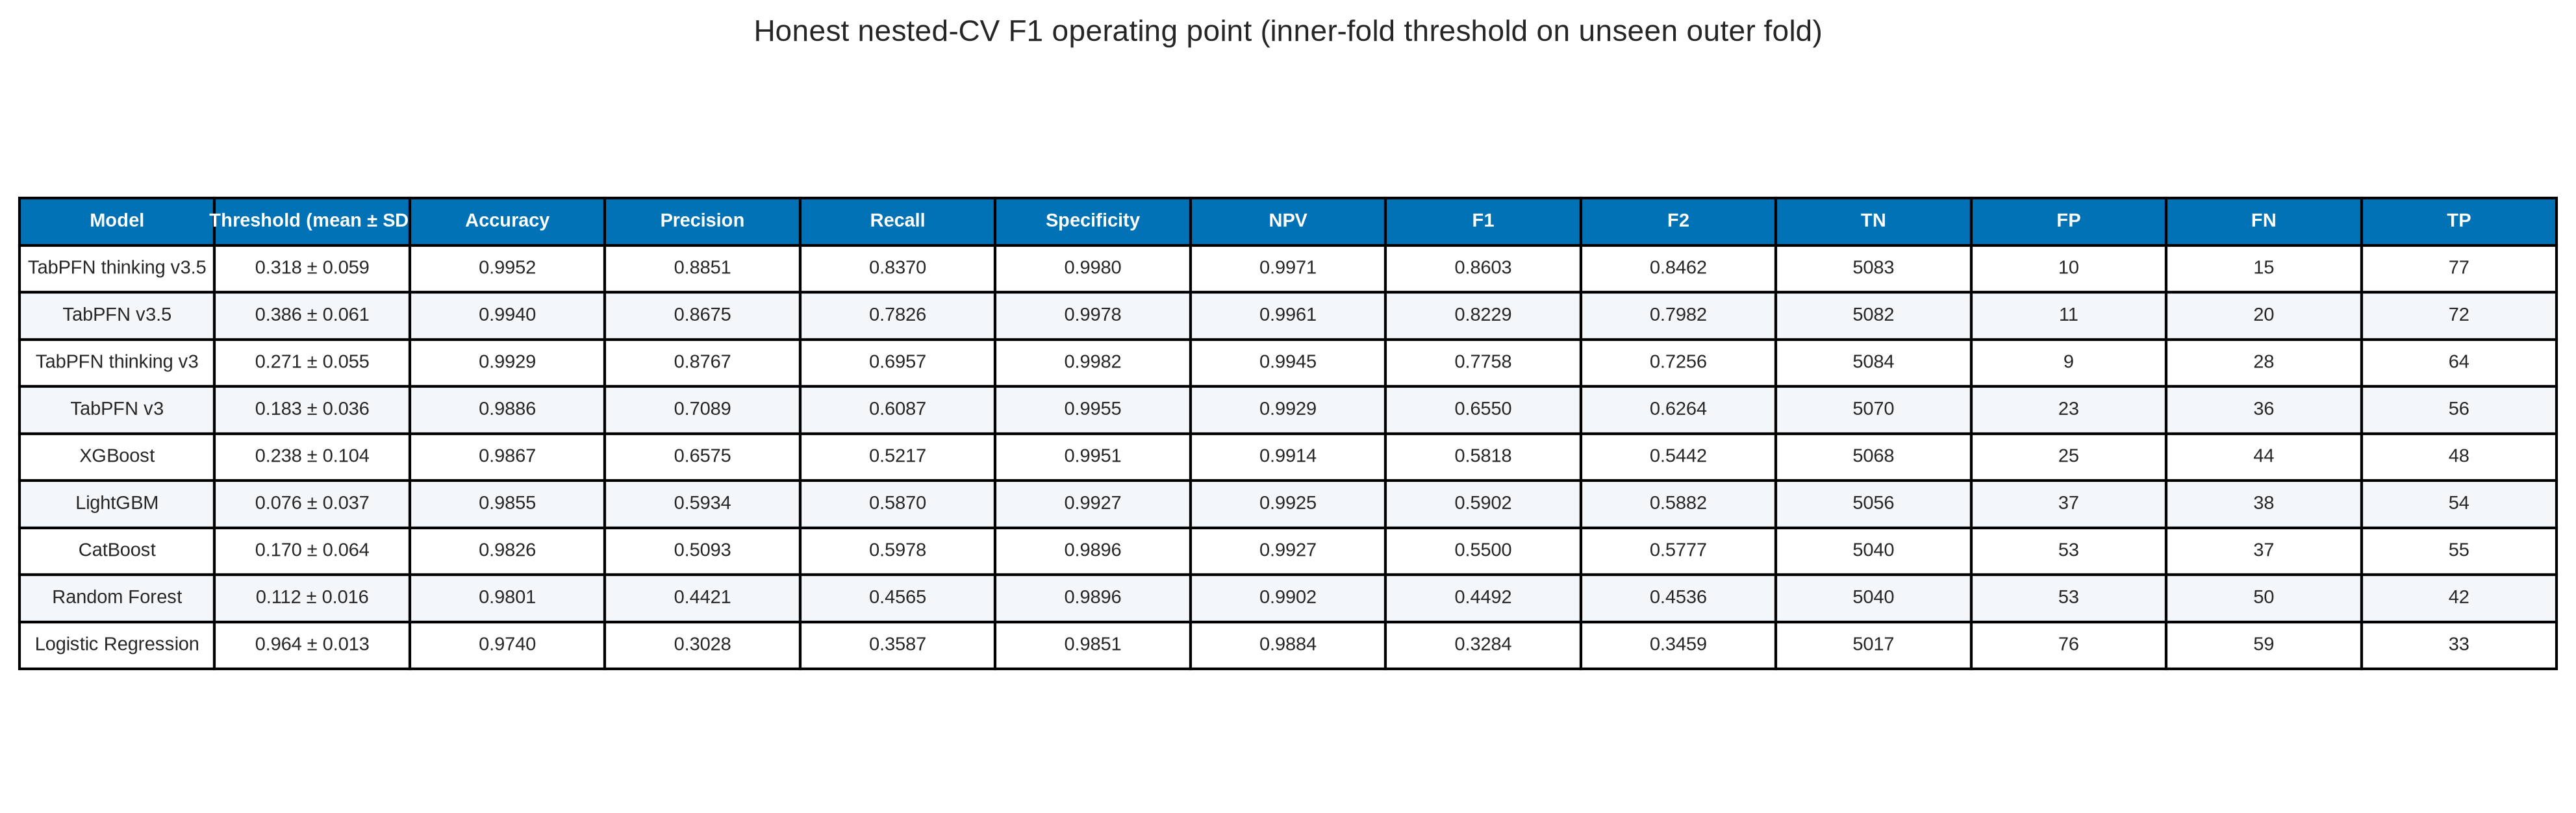
\includegraphics[keepaspectratio,alt={Honest nested operating point}]{../paper_results/04_tabpfn_rating/paper_figures/paper_table2_nested_operating_point.png}}
\caption{Honest nested operating point}
\end{figure}

\begin{figure}
\centering
\pandocbounded{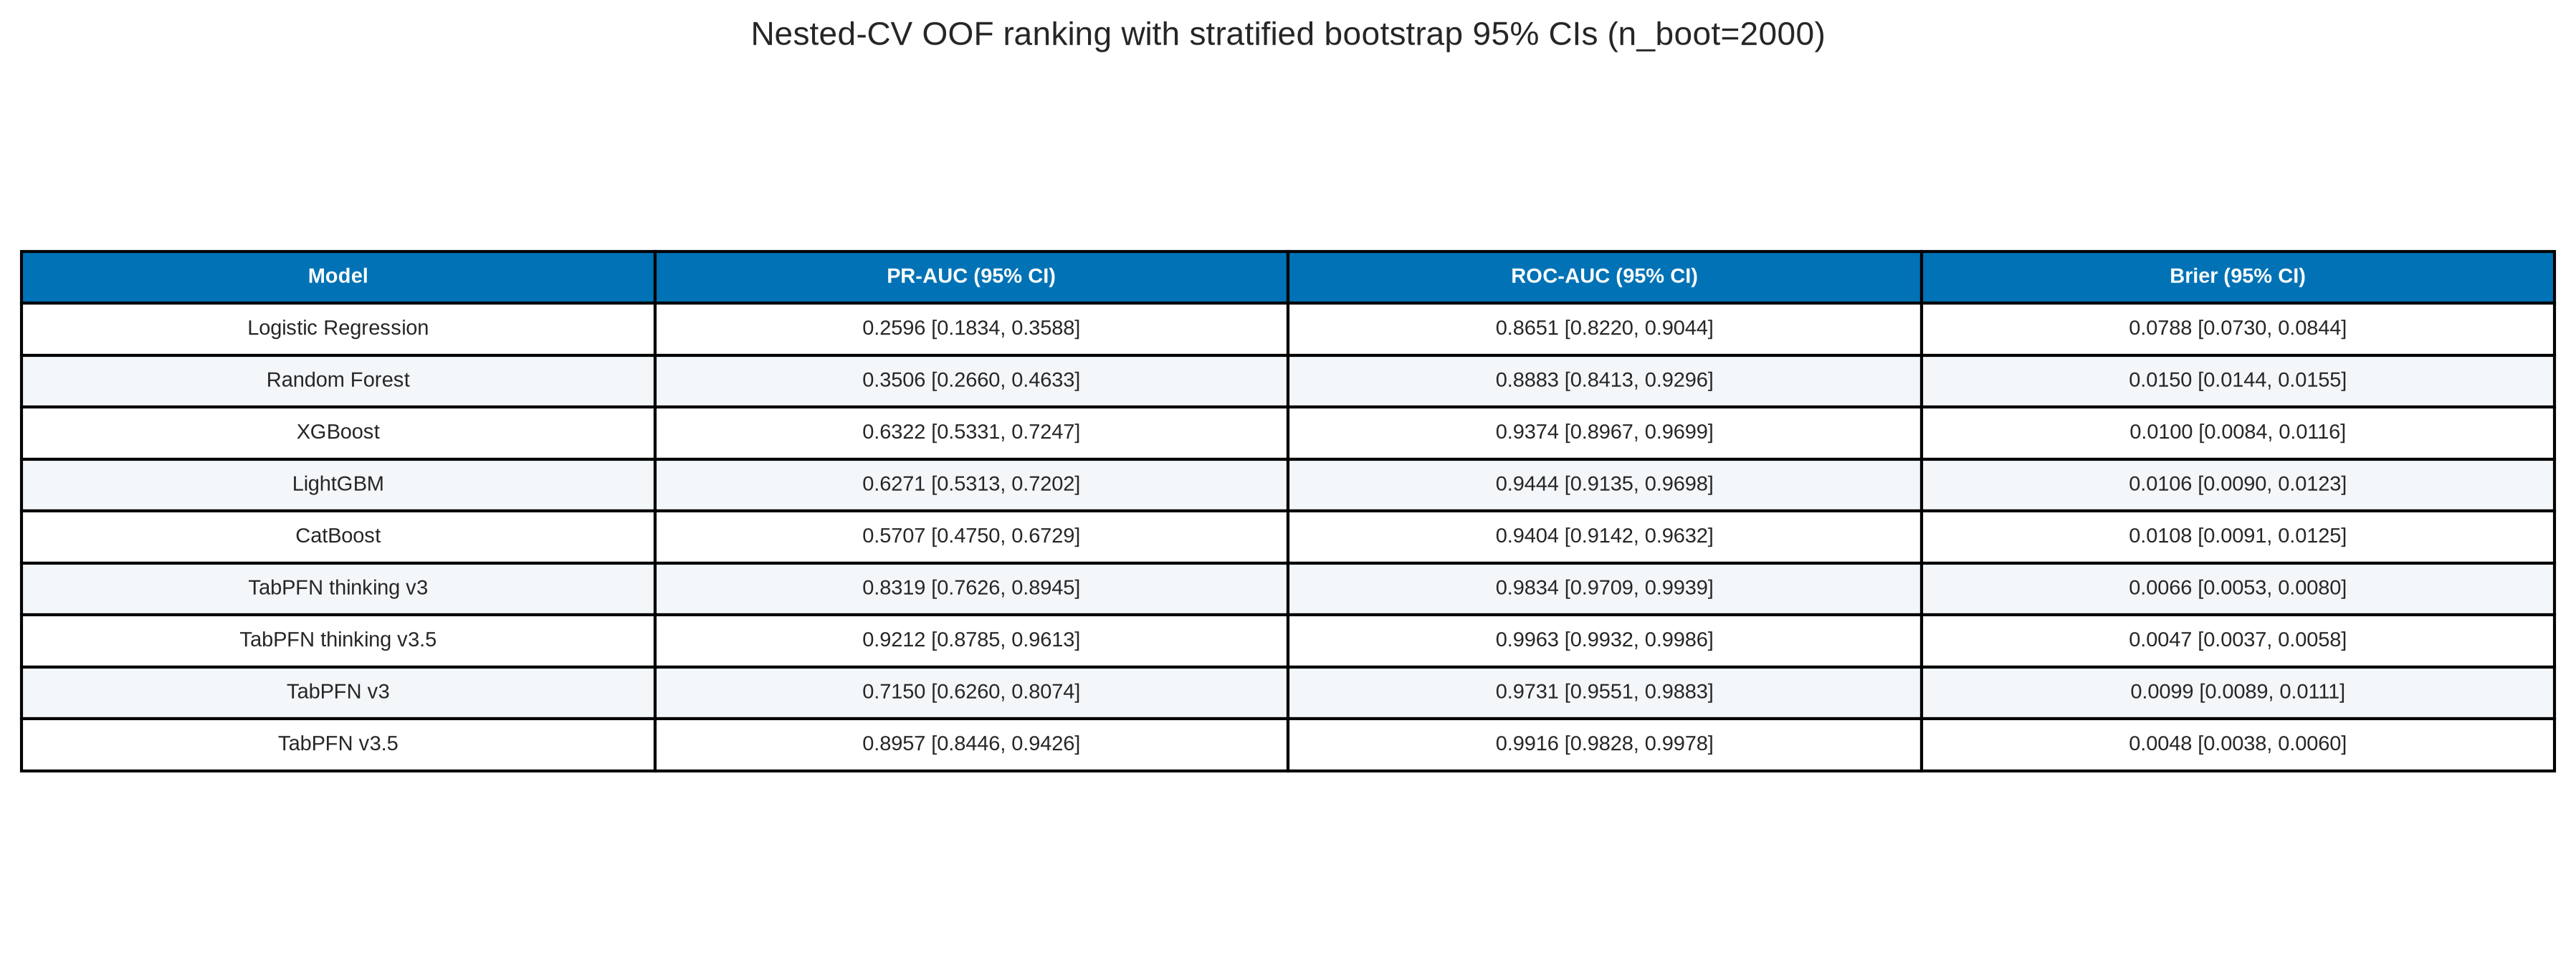
\includegraphics[keepaspectratio,alt={Bootstrap 95\% CIs}]{../paper_results/04_tabpfn_rating/paper_figures/paper_table_s_bootstrap_ci.png}}
\caption{Bootstrap 95\% CIs}
\end{figure}

{\def\LTcaptype{none} % do not increment counter
\begin{longtable}[]{@{}
  >{\raggedright\arraybackslash}p{(\linewidth - 12\tabcolsep) * \real{0.1154}}
  >{\raggedright\arraybackslash}p{(\linewidth - 12\tabcolsep) * \real{0.1154}}
  >{\raggedleft\arraybackslash}p{(\linewidth - 12\tabcolsep) * \real{0.1538}}
  >{\raggedleft\arraybackslash}p{(\linewidth - 12\tabcolsep) * \real{0.1538}}
  >{\raggedleft\arraybackslash}p{(\linewidth - 12\tabcolsep) * \real{0.1538}}
  >{\raggedleft\arraybackslash}p{(\linewidth - 12\tabcolsep) * \real{0.1538}}
  >{\raggedleft\arraybackslash}p{(\linewidth - 12\tabcolsep) * \real{0.1538}}@{}}
\toprule\noalign{}
\begin{minipage}[b]{\linewidth}\raggedright
Model
\end{minipage} & \begin{minipage}[b]{\linewidth}\raggedright
PR-AUC {[}95\% CI{]}
\end{minipage} & \begin{minipage}[b]{\linewidth}\raggedleft
ROC-AUC
\end{minipage} & \begin{minipage}[b]{\linewidth}\raggedleft
Brier
\end{minipage} & \begin{minipage}[b]{\linewidth}\raggedleft
Sensitivity
\end{minipage} & \begin{minipage}[b]{\linewidth}\raggedleft
Precision
\end{minipage} & \begin{minipage}[b]{\linewidth}\raggedleft
F1
\end{minipage} \\
\midrule\noalign{}
\endhead
\bottomrule\noalign{}
\endlastfoot
TabPFN thinking v3.5 & \textbf{0.9212} {[}0.8785, 0.9613{]} & 0.9963 &
0.0047 & 0.8370 & 0.8851 & 0.8603 \\
TabPFN v3.5 & 0.8957 {[}0.8446, 0.9426{]} & 0.9916 & 0.0048 & 0.7826 &
0.8675 & 0.8229 \\
TabPFN thinking v3 & 0.8319 {[}0.7626, 0.8945{]} & 0.9834 & 0.0066 &
0.6957 & 0.8767 & 0.7758 \\
TabPFN v3 & 0.7150 {[}0.6260, 0.8074{]} & 0.9731 & 0.0099 & 0.6087 &
0.7089 & 0.6550 \\
XGBoost & 0.6322 {[}0.5331, 0.7247{]} & 0.9374 & 0.0100 & 0.5217 &
0.6575 & 0.5818 \\
LightGBM & 0.6271 {[}0.5313, 0.7202{]} & 0.9444 & 0.0106 & 0.5870 &
0.5934 & 0.5902 \\
CatBoost & 0.5707 {[}0.4750, 0.6729{]} & 0.9404 & 0.0108 & 0.5978 &
0.5093 & 0.5500 \\
Random forest & 0.3506 {[}0.2660, 0.4633{]} & 0.8883 & 0.0150 & 0.4565 &
0.4421 & 0.4492 \\
Logistic regression & 0.2596 {[}0.1834, 0.3588{]} & 0.8651 & 0.0788 &
0.3587 & 0.3028 & 0.3284 \\
\end{longtable}
}

Thinking v3.5 nested 2×2: 5083/10/15/77. TabPFN v3.5: 5082/11/20/72.
LightGBM: 5056/37/38/54. Frozen Wang integer score (not a nested arm):
ROC-AUC 0.8013, PR-AUC 0.1032.

\begin{center}\rule{0.5\linewidth}{0.5pt}\end{center}

\subsection{Table 4. Eight-seed forward SFS rankings (train, local
TabPFN
v3.5)}\label{table-4.-eight-seed-forward-sfs-rankings-train-local-tabpfn-v3.5}

Keep 10 of 80 columns; 5-fold CV; average precision;
\texttt{STABILITY\_N\_SEEDS=8}. Train n = 3,629. \texttt{WBC} dropped.
Not a nested-CV feature mask.

\begin{figure}
\centering
\pandocbounded{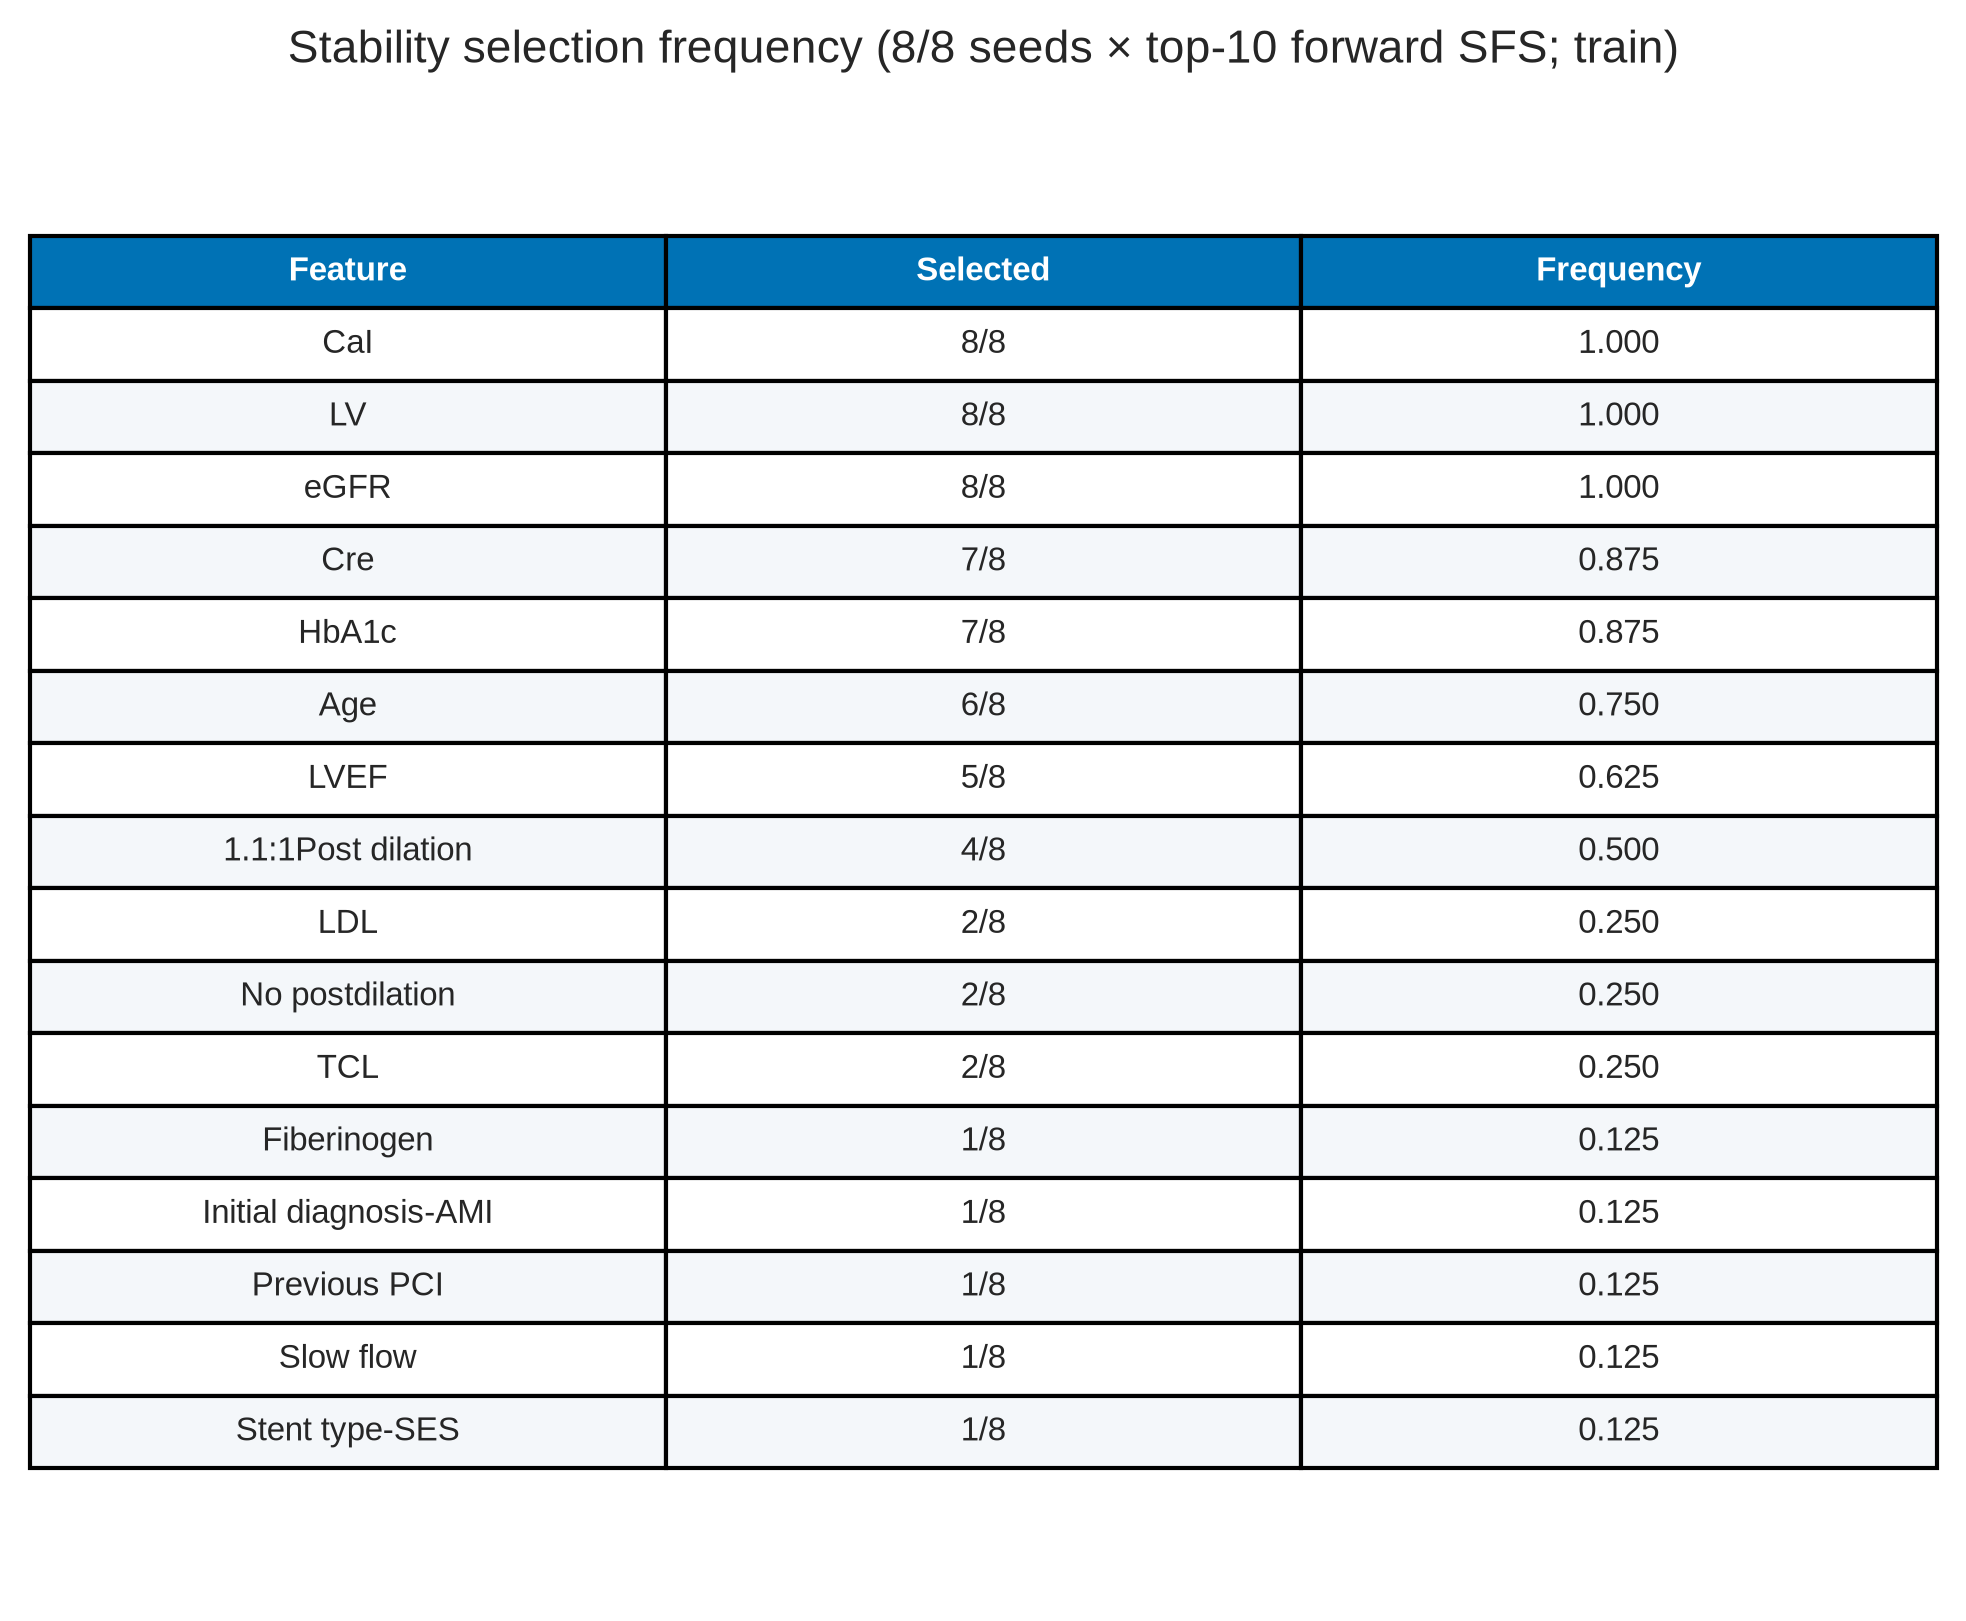
\includegraphics[keepaspectratio,alt={Table 4. SFS stability}]{../paper_results/05_tabpfn_interpretability/paper_figures/paper_table2_stability.png}}
\caption{Table 4. SFS stability}
\end{figure}

{\def\LTcaptype{none} % do not increment counter
\begin{longtable}[]{@{}rllr@{}}
\toprule\noalign{}
Rank & Feature & Selected & Frequency \\
\midrule\noalign{}
\endhead
\bottomrule\noalign{}
\endlastfoot
1 & CaI & 8/8 & 1.000 \\
2 & LV & 8/8 & 1.000 \\
3 & eGFR & 8/8 & 1.000 \\
4 & Cre & 7/8 & 0.875 \\
5 & HbA1c & 7/8 & 0.875 \\
6 & Age & 6/8 & 0.750 \\
7 & LVEF & 5/8 & 0.625 \\
8 & 1.1:1Post dilation & 4/8 & 0.500 \\
9 & LDL & 2/8 & 0.250 \\
10 & No postdilation & 2/8 & 0.250 \\
11 & TCL & 2/8 & 0.250 \\
12 & Fiberinogen & 1/8 & 0.125 \\
13 & Initial diagnosis-AMI & 1/8 & 0.125 \\
14 & Previous PCI & 1/8 & 0.125 \\
15 & Slow flow & 1/8 & 0.125 \\
16 & Stent type-SES & 1/8 & 0.125 \\
\end{longtable}
}

Held-out mean(\textbar SHAP\textbar) for the 8/8 names (1,556 rows):
eGFR 1.2288, CaI 1.0867, LV 0.4828 (Cre 0.8093 is 7/8 SFS).

\begin{center}\rule{0.5\linewidth}{0.5pt}\end{center}

\subsection{Interpretability figures}\label{interpretability-figures}

\textbf{Mutual information (train).}

\begin{figure}
\centering
\pandocbounded{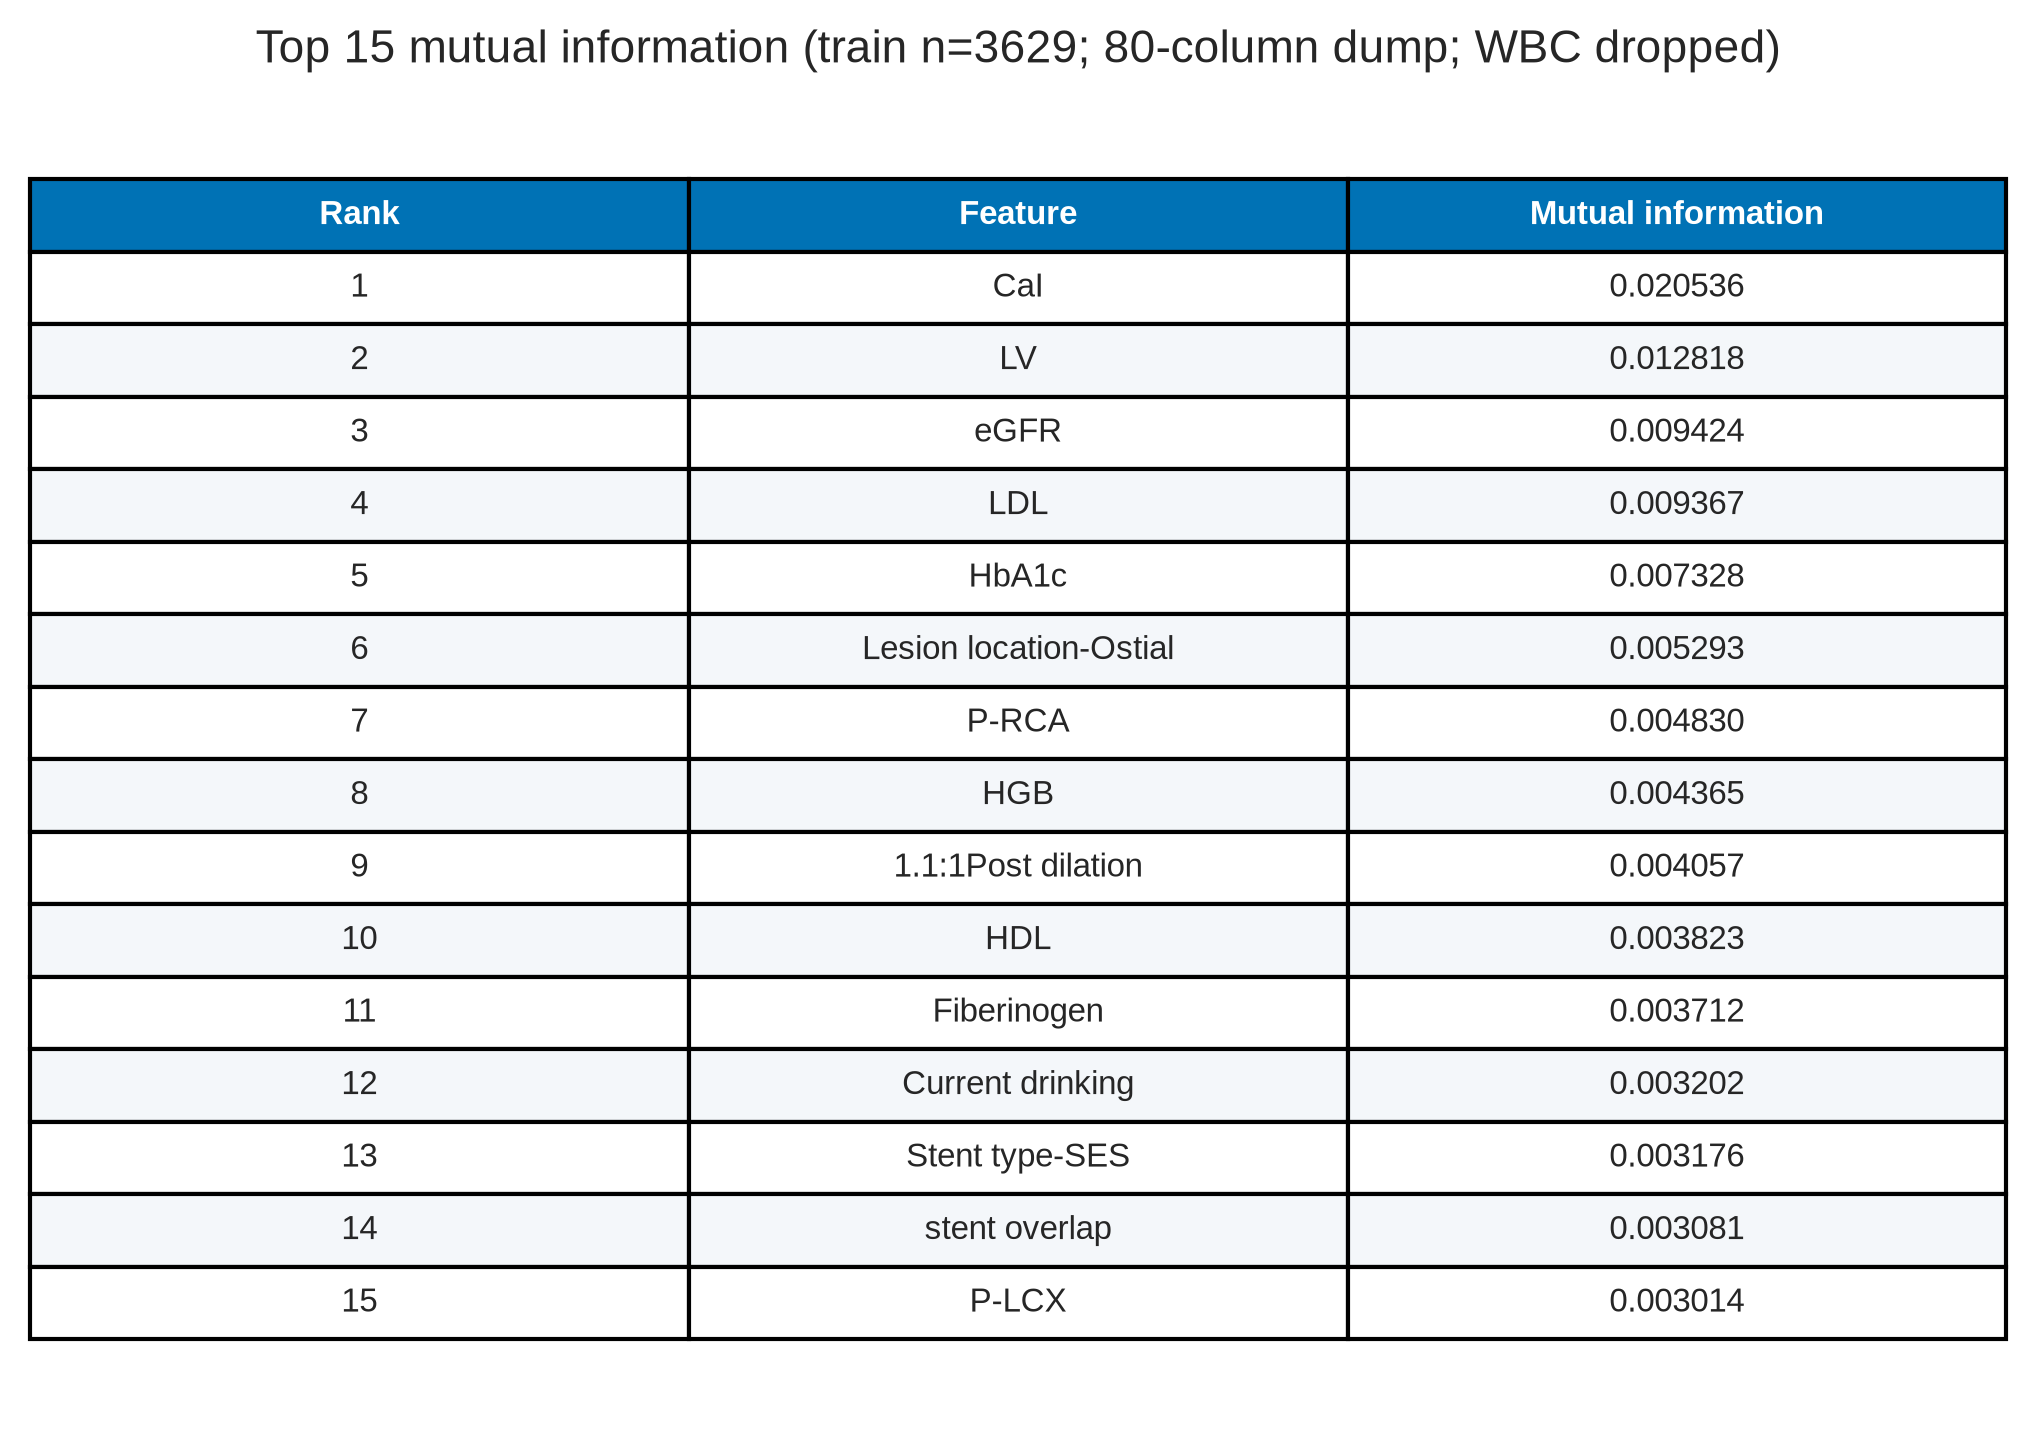
\includegraphics[keepaspectratio,alt={Table. Top 15 mutual information}]{../paper_results/05_tabpfn_interpretability/paper_figures/paper_table1_mutual_info.png}}
\caption{Table. Top 15 mutual information}
\end{figure}

\textbf{Figure. Continuous PDP} (train; empirical prior; not nested-CV
risk).

\begin{figure}
\centering
\pandocbounded{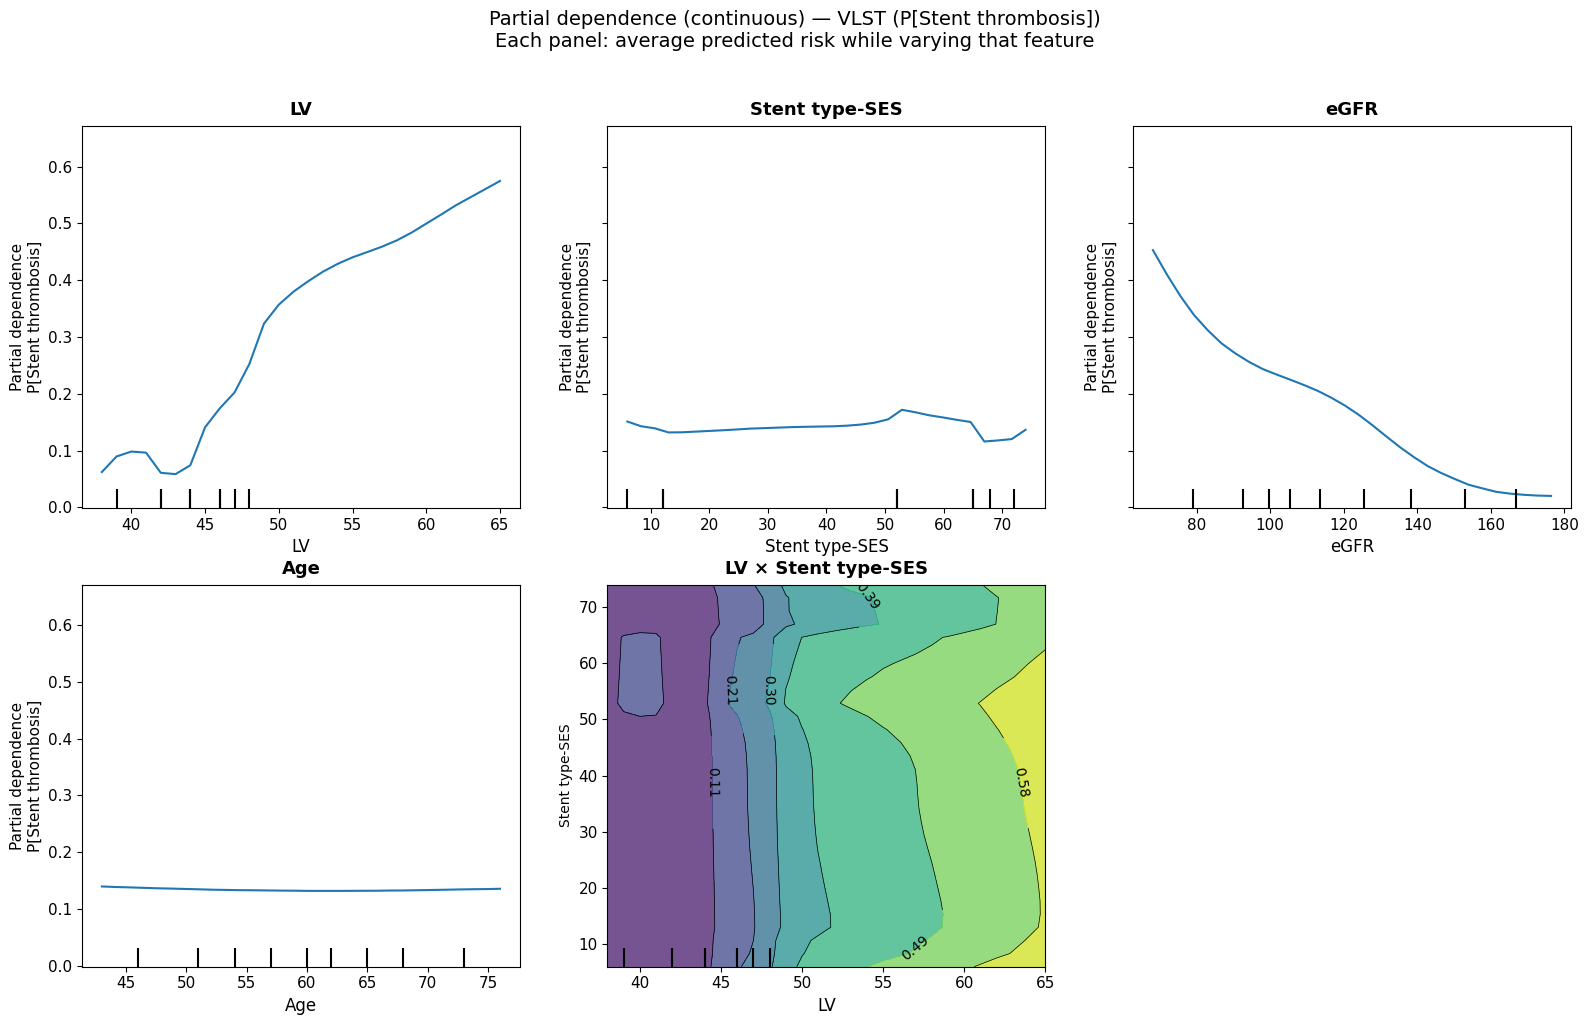
\includegraphics[keepaspectratio,alt={Figure. Continuous PDP}]{../paper_results/05_tabpfn_interpretability/paper_figures/paper_fig1_pdp_continuous.png}}
\caption{Figure. Continuous PDP}
\end{figure}

\textbf{Figure. Binary PDP.}

\begin{figure}
\centering
\pandocbounded{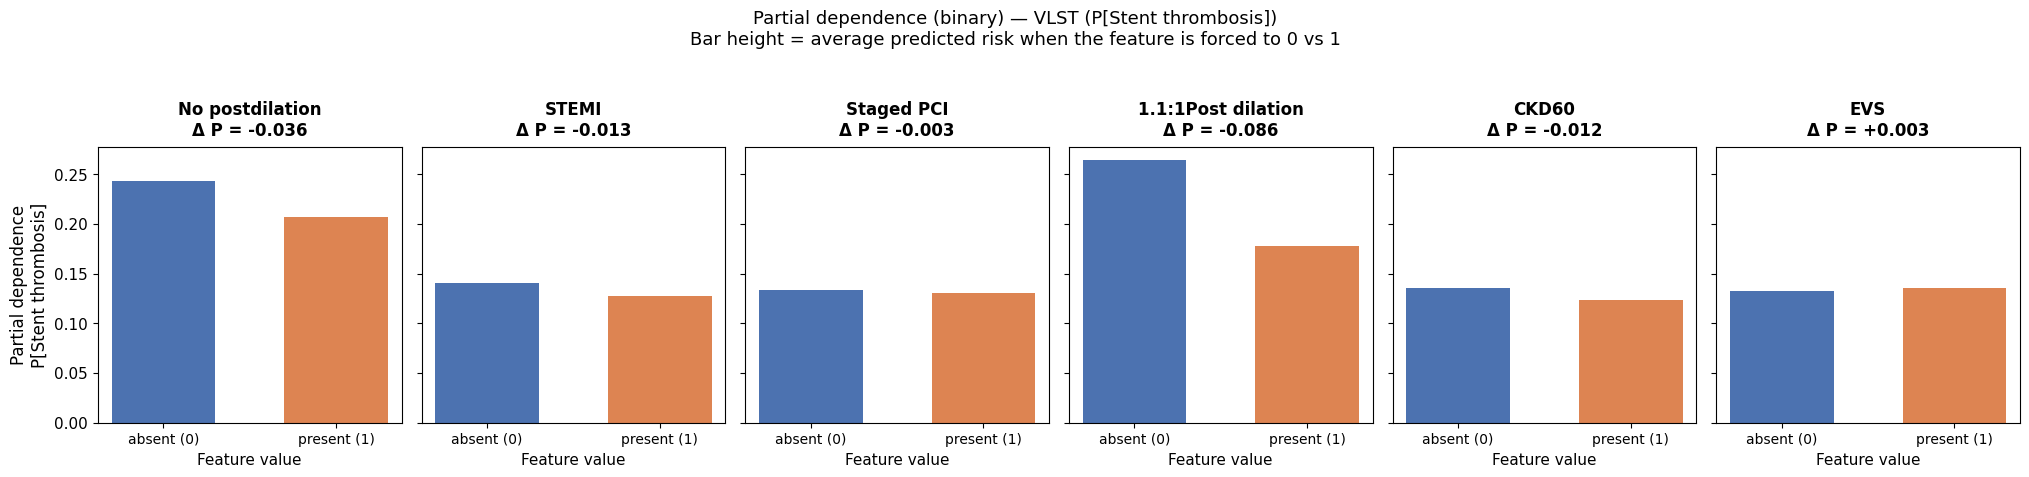
\includegraphics[keepaspectratio,alt={Figure. Binary PDP}]{../paper_results/05_tabpfn_interpretability/paper_figures/paper_fig2_pdp_binary.png}}
\caption{Figure. Binary PDP}
\end{figure}

\textbf{Figure. SHAP summary} (1,556 held-out rows).

\begin{figure}
\centering
\pandocbounded{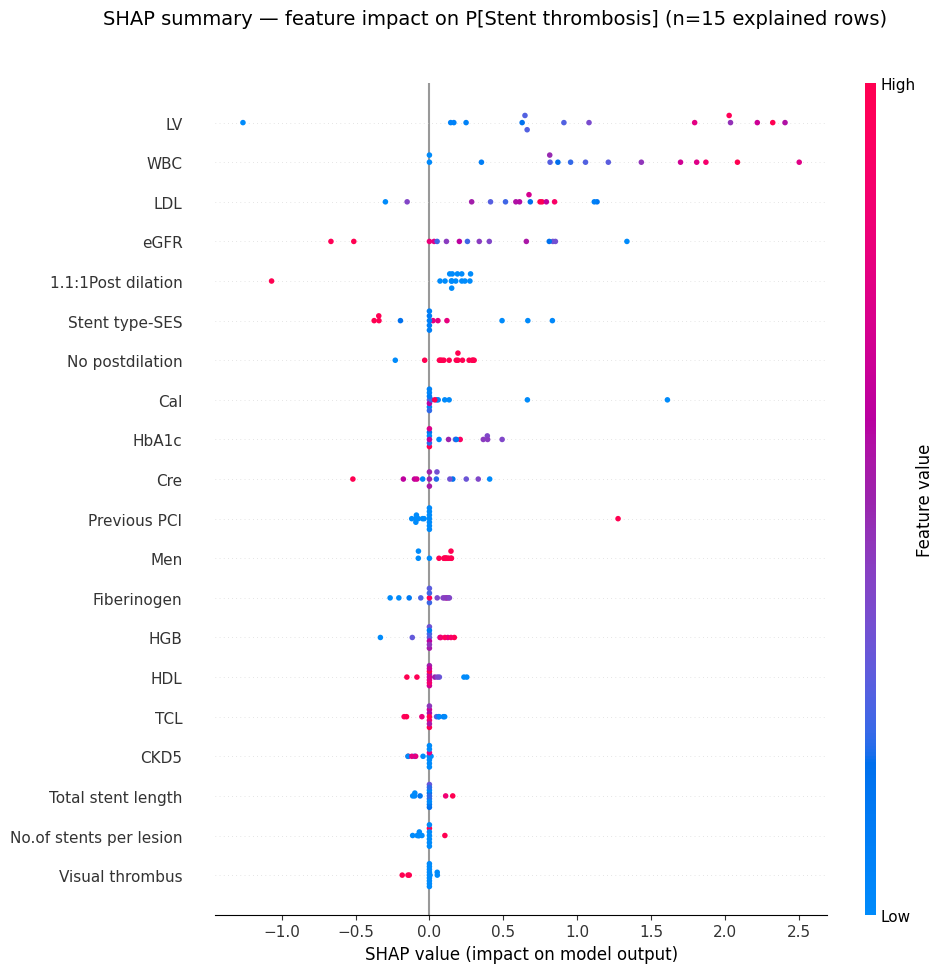
\includegraphics[keepaspectratio,alt={Figure. SHAP summary}]{../paper_results/05_tabpfn_interpretability/paper_figures/paper_fig3_shap_summary.png}}
\caption{Figure. SHAP summary}
\end{figure}

\textbf{Figure. Mean \textbar SHAP\textbar{} bar.} Leading: eGFR 1.2288,
CaI 1.0867, Cre 0.8093, LV 0.4828.

\begin{figure}
\centering
\pandocbounded{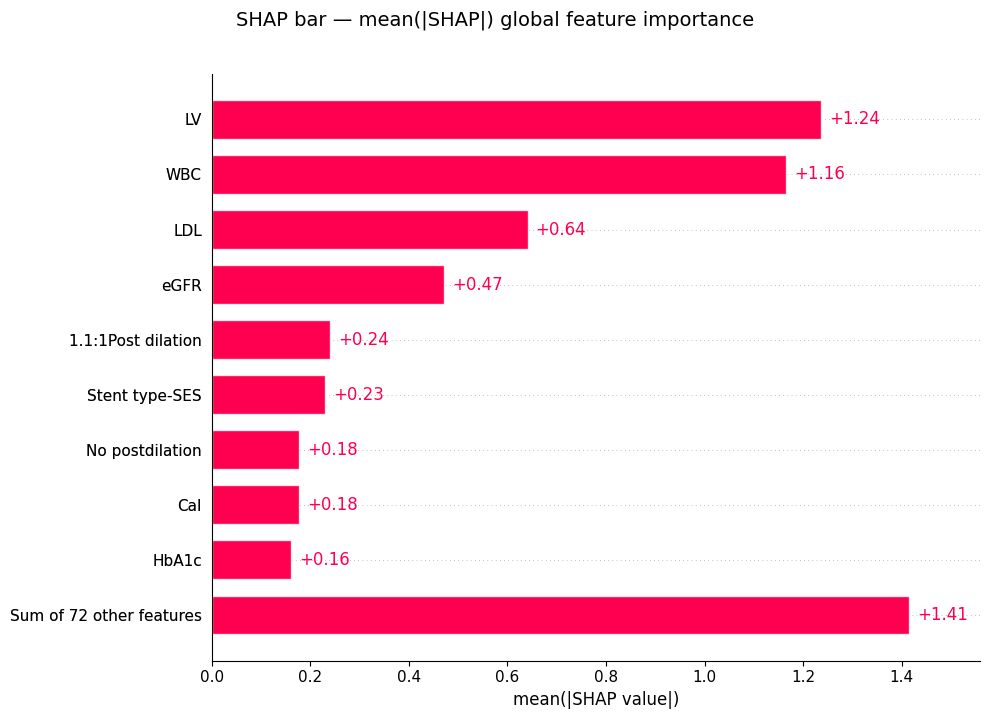
\includegraphics[keepaspectratio,alt={Figure. SHAP bar}]{../paper_results/05_tabpfn_interpretability/paper_figures/paper_fig5_shap_bar.png}}
\caption{Figure. SHAP bar}
\end{figure}

\textbf{Figure. SHAP beeswarm.}

\begin{figure}
\centering
\pandocbounded{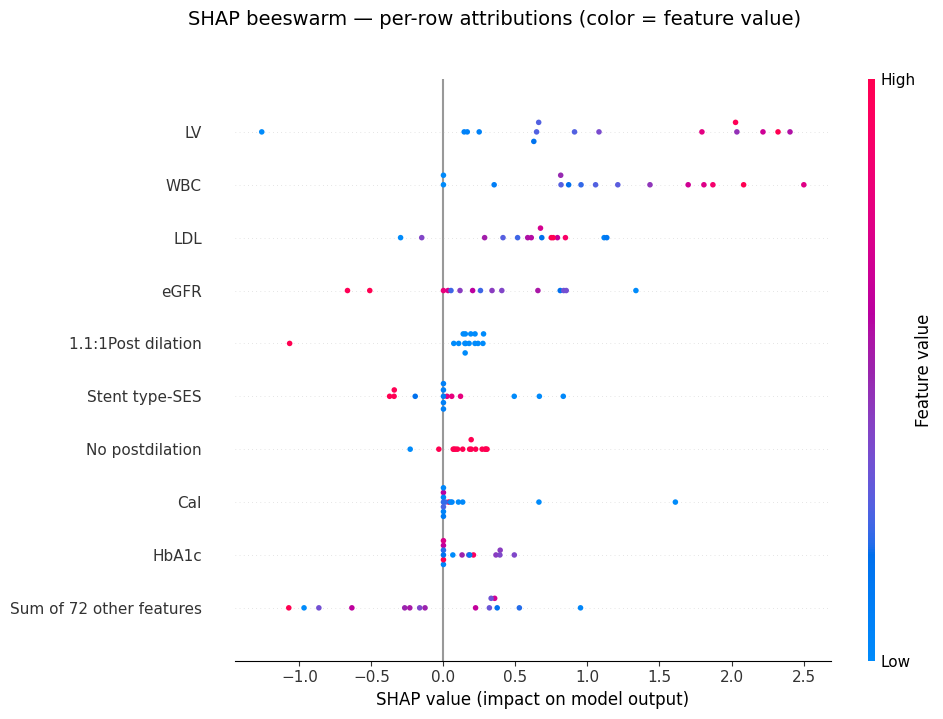
\includegraphics[keepaspectratio,alt={Figure. SHAP beeswarm}]{../paper_results/05_tabpfn_interpretability/paper_figures/paper_fig6_shap_beeswarm.png}}
\caption{Figure. SHAP beeswarm}
\end{figure}

\textbf{Figure. One-row waterfall} (cohort row 5176).

\begin{figure}
\centering
\pandocbounded{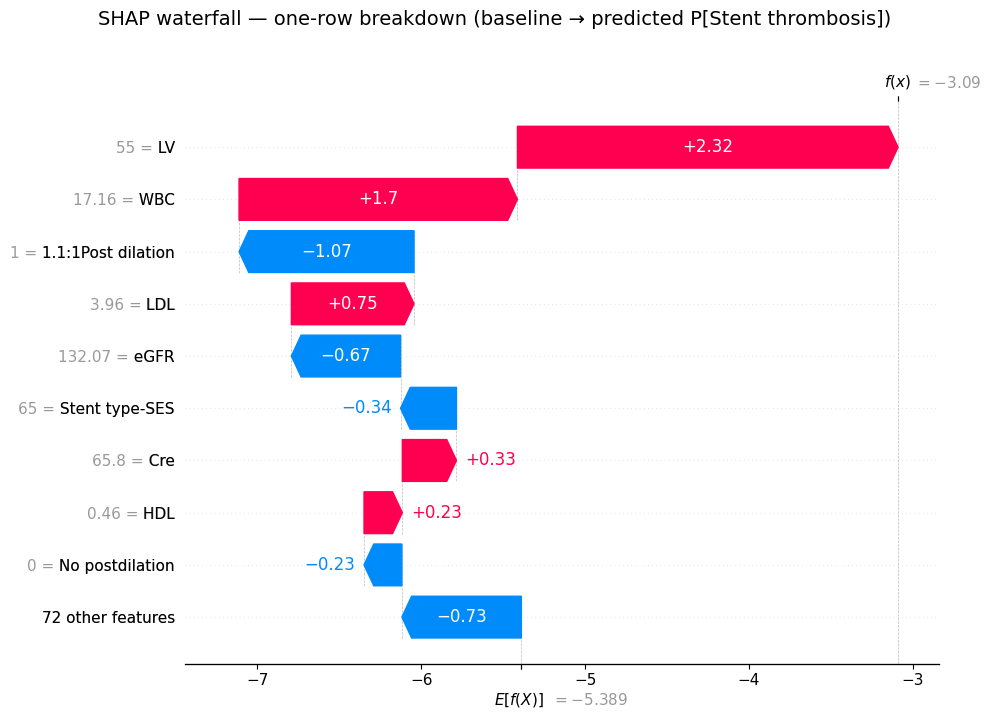
\includegraphics[keepaspectratio,alt={Figure. SHAP waterfall}]{../paper_results/05_tabpfn_interpretability/paper_figures/paper_fig7_shap_waterfall.png}}
\caption{Figure. SHAP waterfall}
\end{figure}

\textbf{Figure. \emph{k}-SII network} (same one VLST=1 row; not a cohort
interaction screen).

\begin{figure}
\centering
\pandocbounded{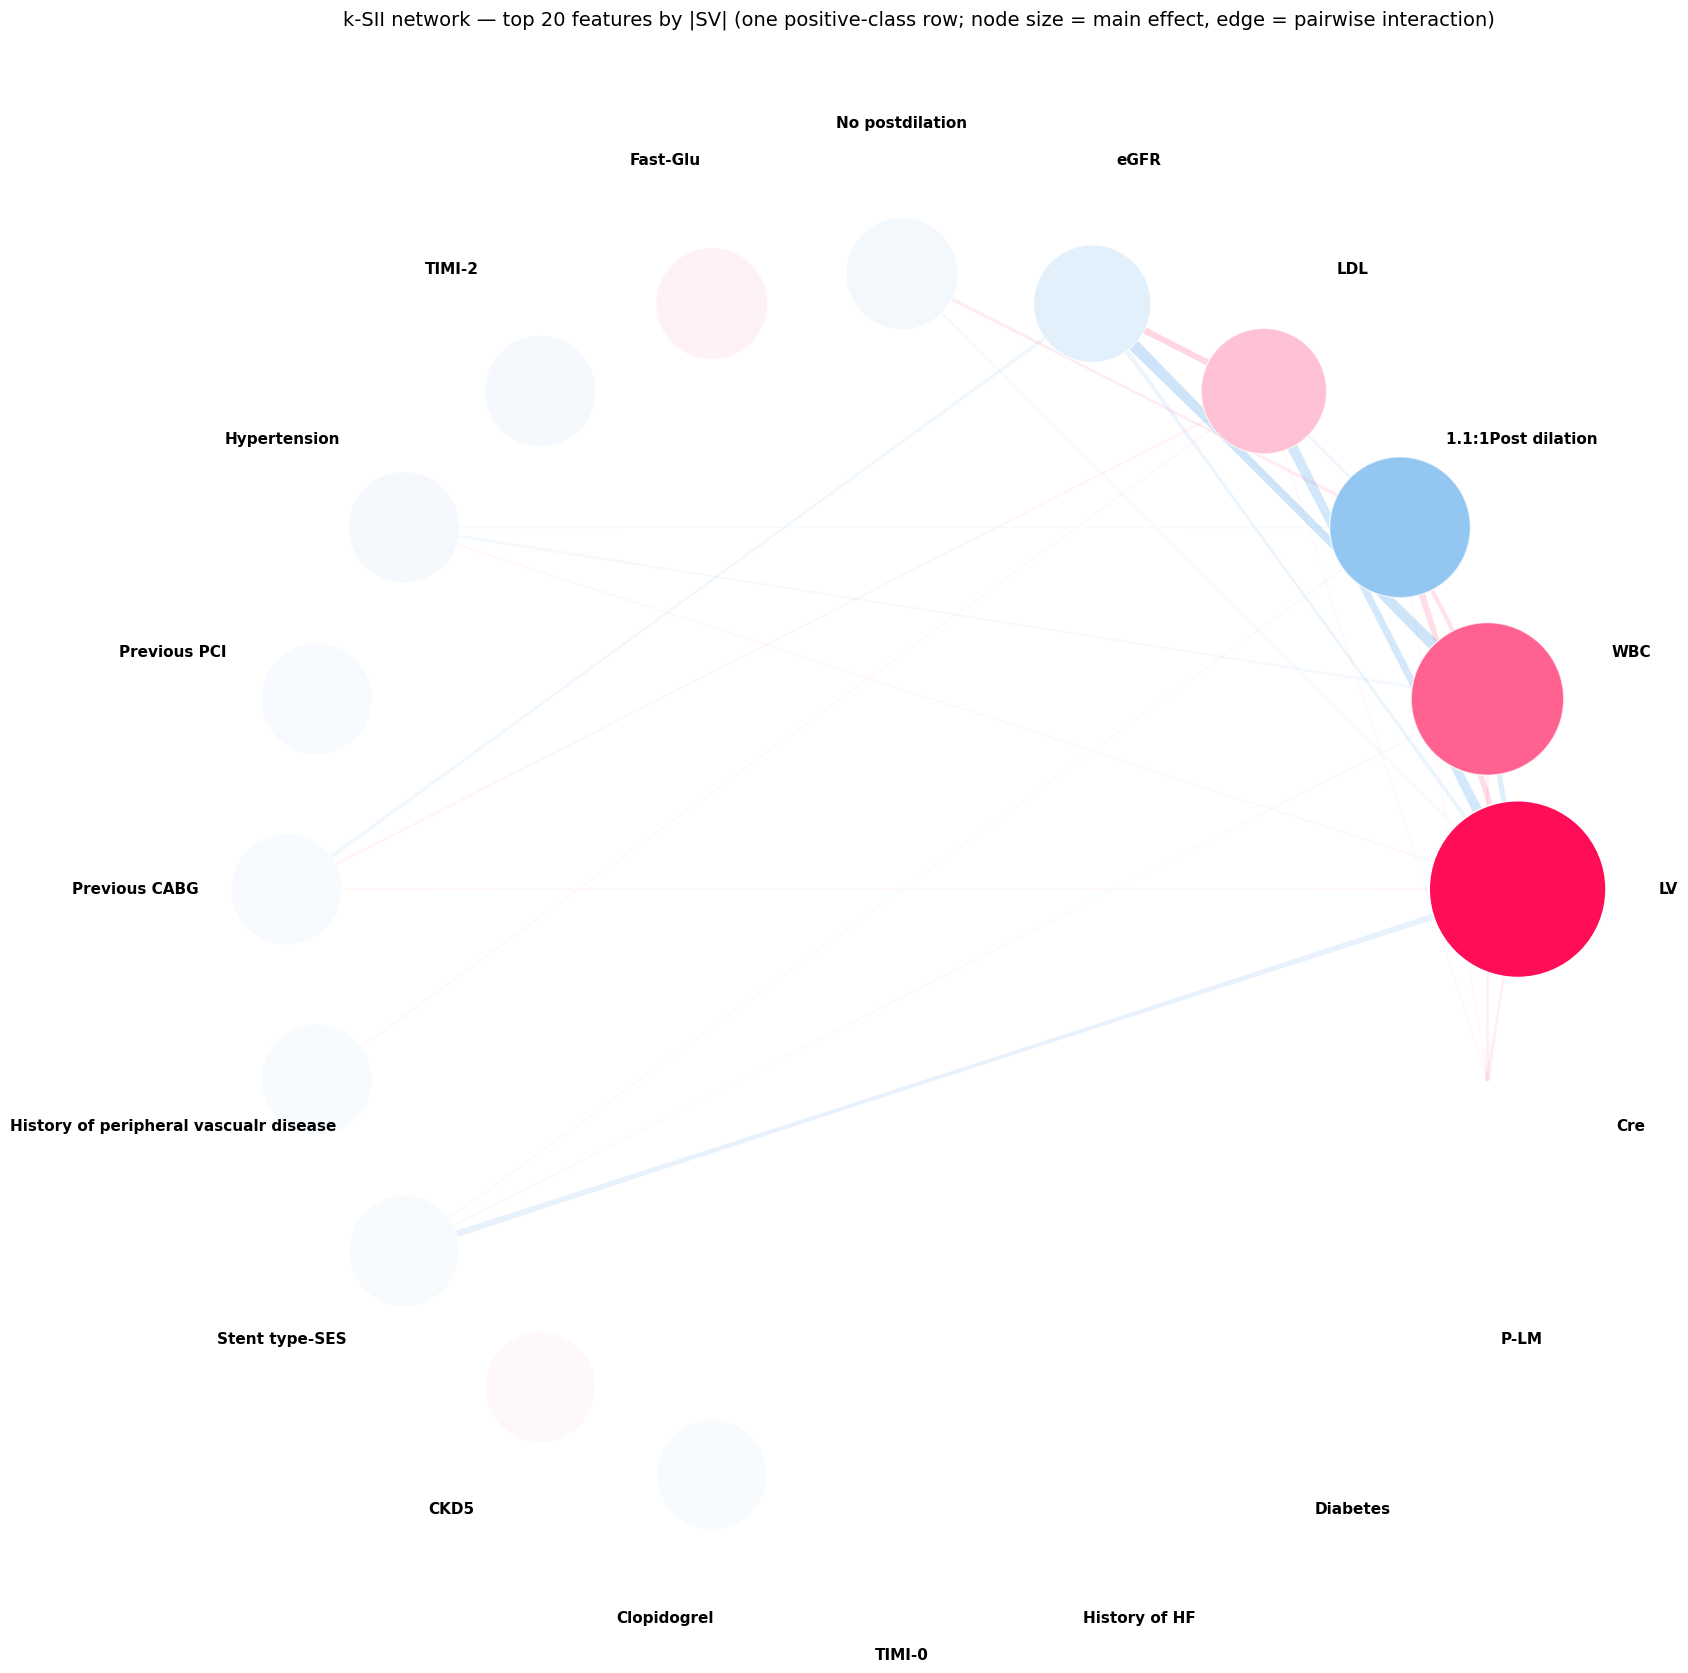
\includegraphics[keepaspectratio,alt={Figure. k-SII network}]{../paper_results/05_tabpfn_interpretability/paper_figures/paper_fig8_ksii_network.png}}
\caption{Figure. k-SII network}
\end{figure}

\textbf{Figure. Consensus ranking} (train MI + train SFS + held-out
SHAP).

\begin{figure}
\centering
\pandocbounded{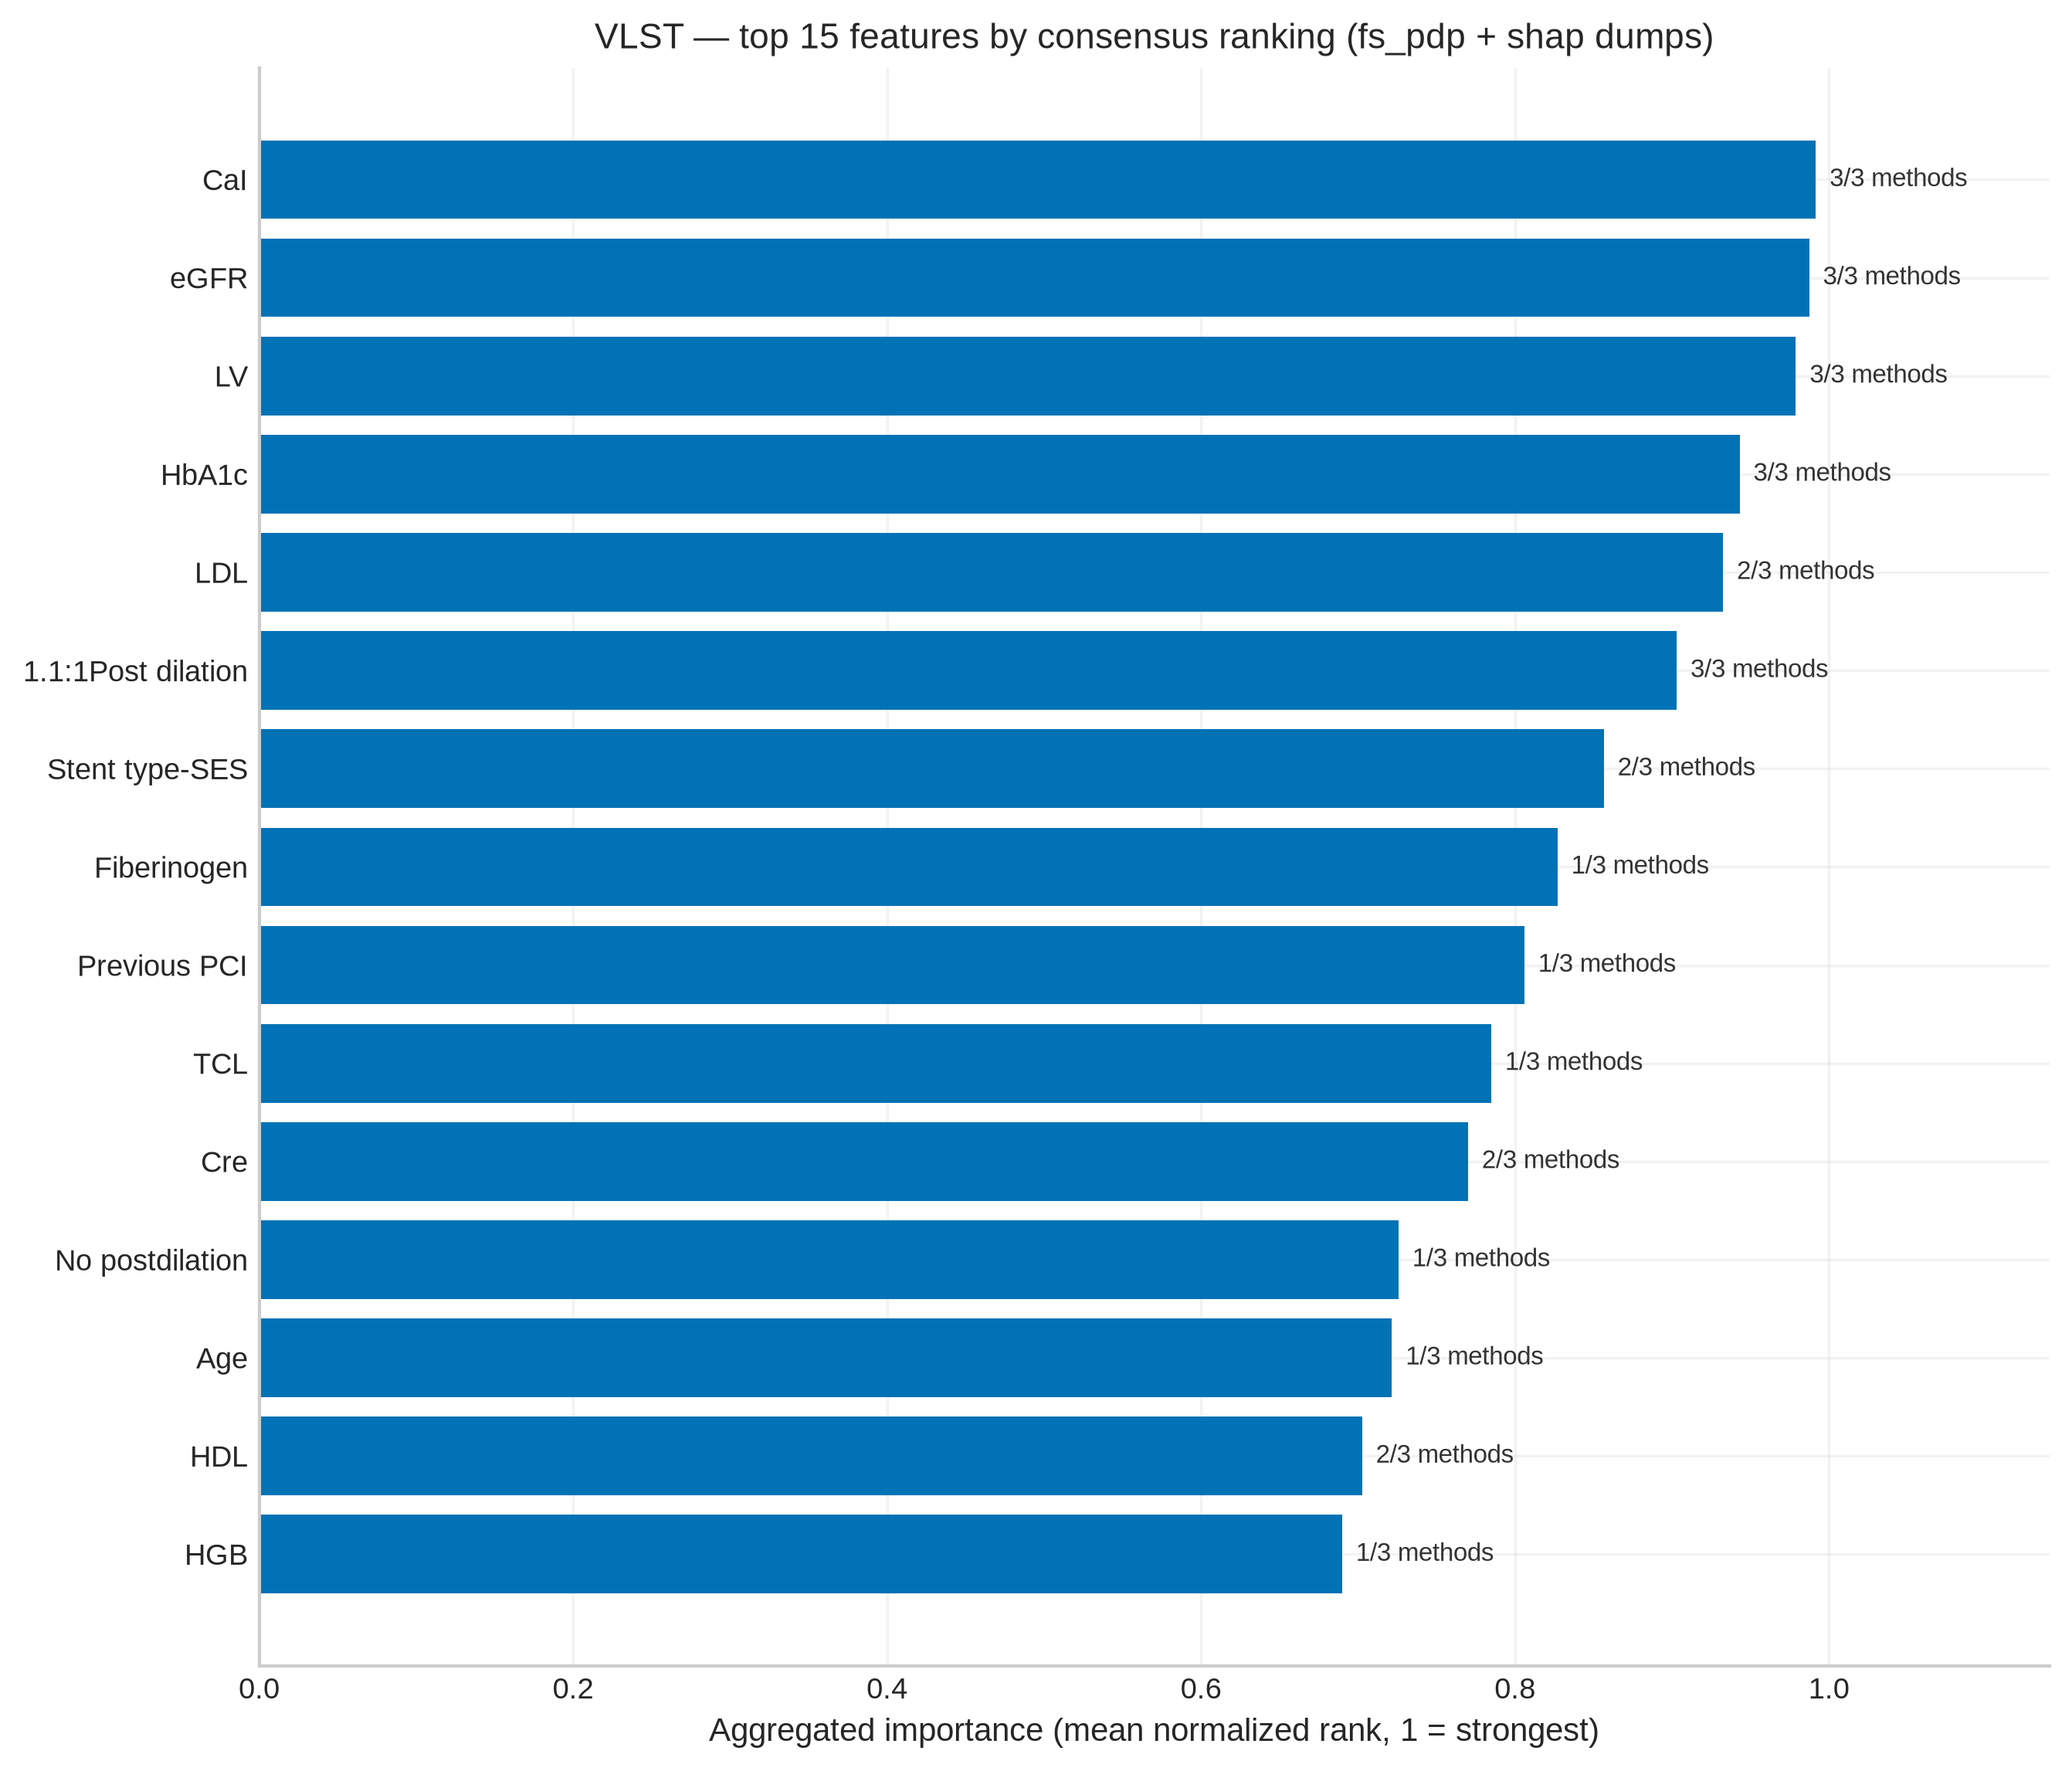
\includegraphics[keepaspectratio,alt={Figure. Consensus ranking}]{../paper_results/05_tabpfn_interpretability/paper_figures/paper_fig13_consensus_ranking.png}}
\caption{Figure. Consensus ranking}
\end{figure}

\begin{figure}
\centering
\pandocbounded{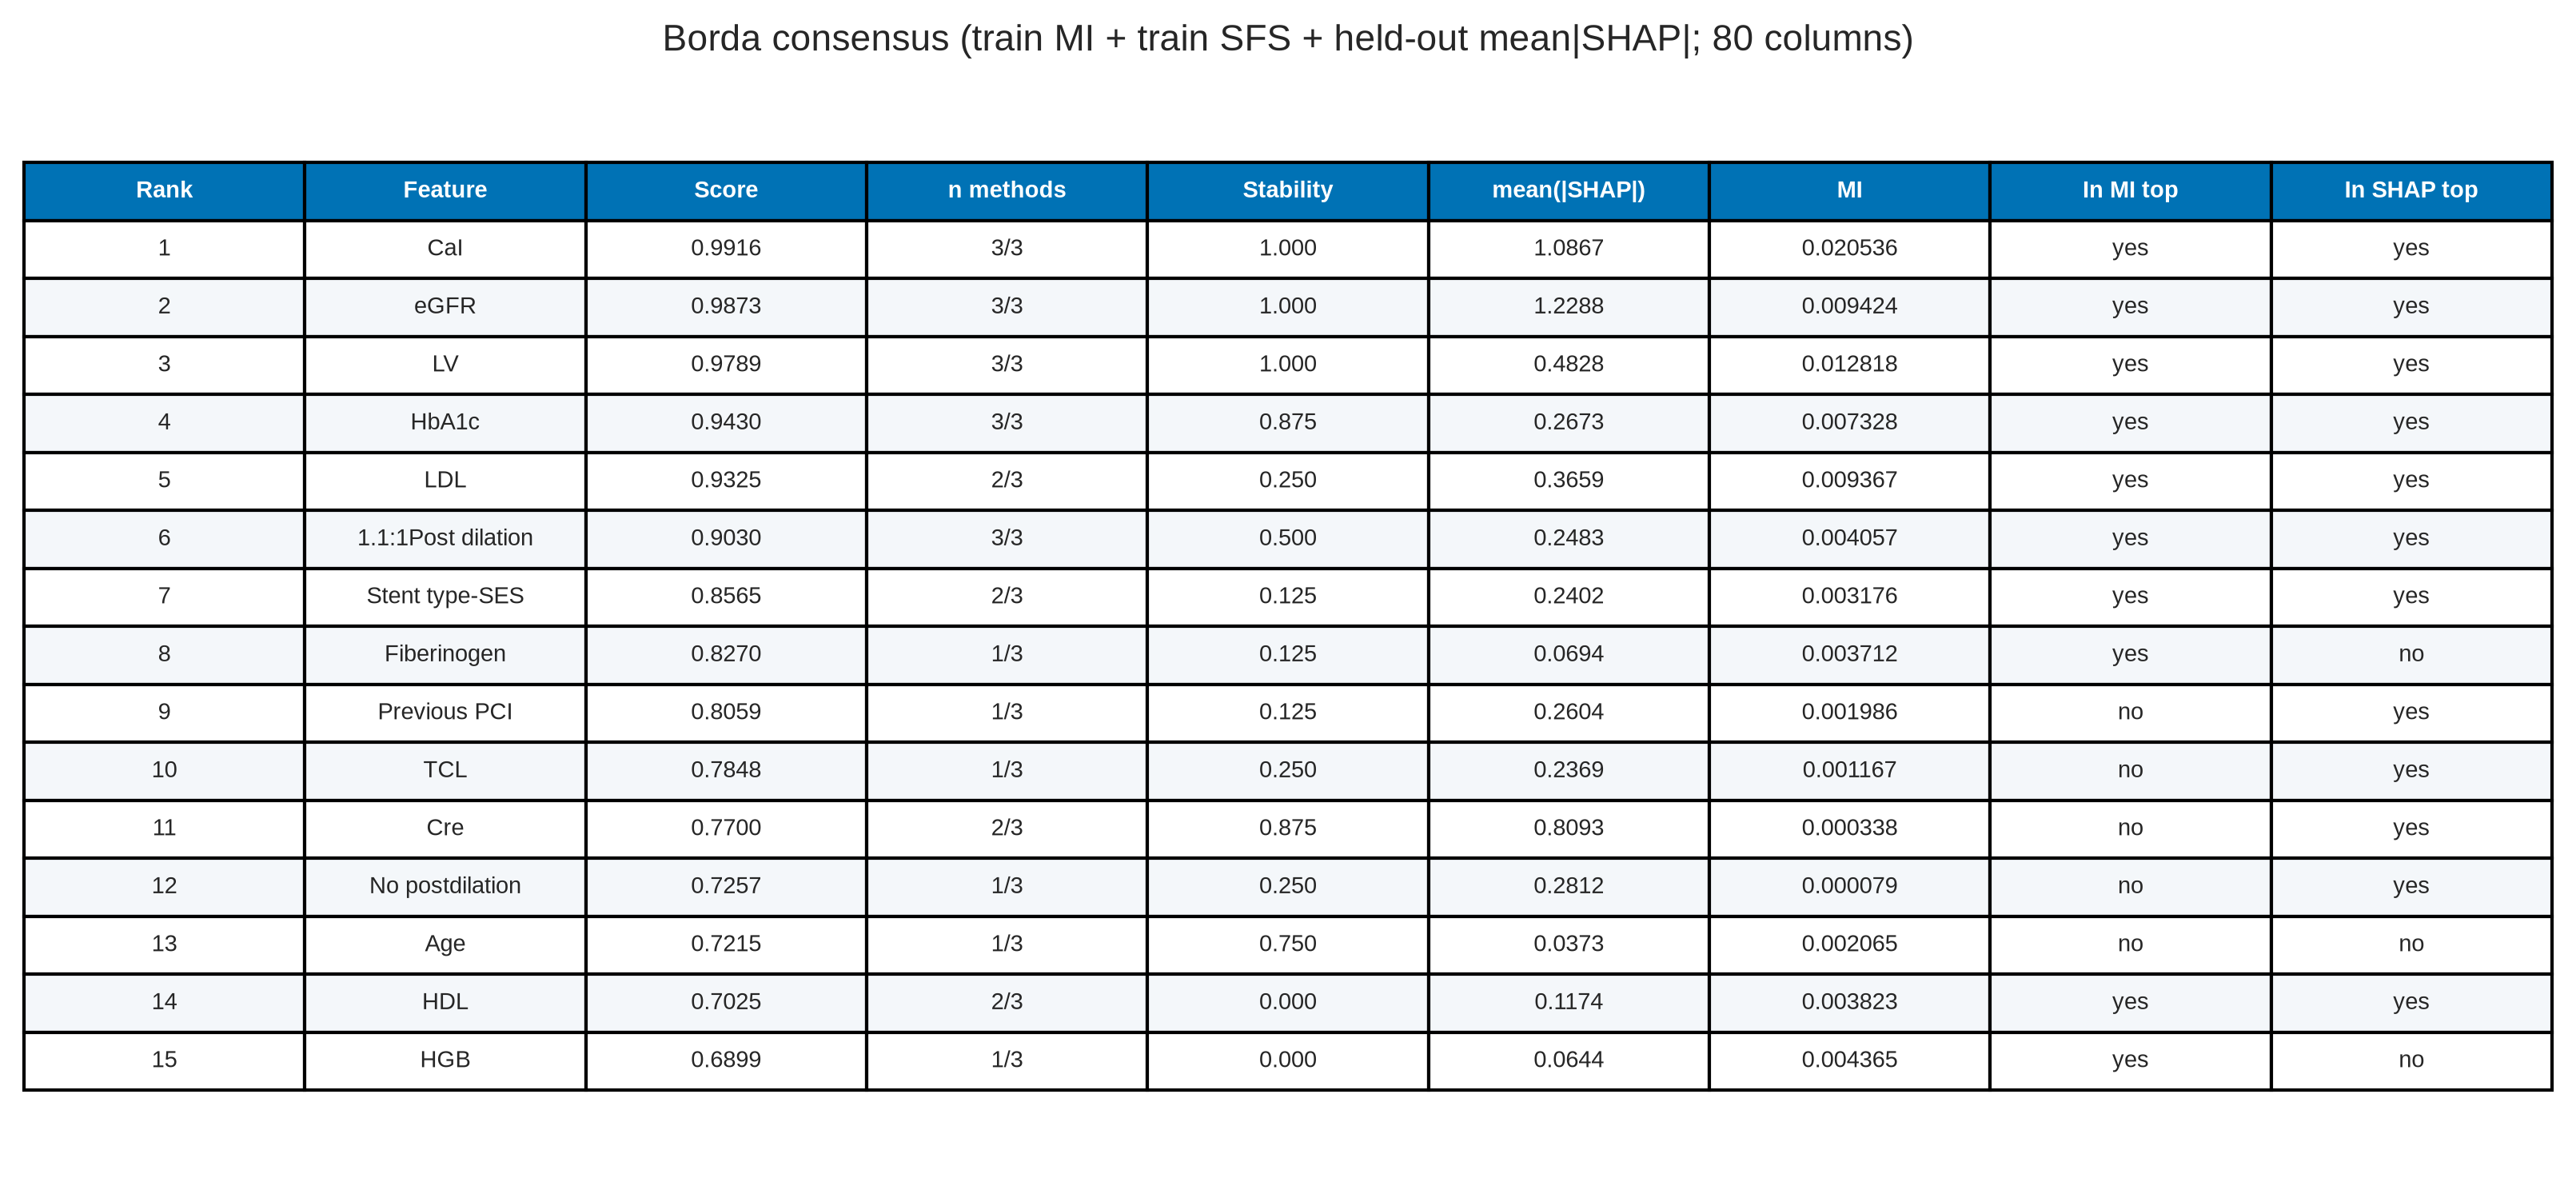
\includegraphics[keepaspectratio,alt={Table. Consensus report}]{../paper_results/05_tabpfn_interpretability/paper_figures/paper_table5_consensus.png}}
\caption{Table. Consensus report}
\end{figure}

Do not quote pooled confusion matrices
(\texttt{paper\_fig3\_confusion\_matrices.png}) as nested operating
points.

\end{document}
